%% Before beginning to type your dissertation, read the formatting guide, 
%% which can be found at http://grad.msu.edu/etd/docs/formattingguide.pdf
%% Also get the latest version of  msuphddissertation.cls and the template file
%% at http://www.math.msu.edu/~weil/MSU_Ph.D._Dissertation.zip
%% Send questions to weil@math.msu.edu
\documentclass{msuphddissertation}
\usepackage{amssymb, amsmath}
%\usepackage{subcaption}
\usepackage{graphicx}
\usepackage{url}
%% Insert packages you wish to use except setspace and subfig. 
%% Those packages are loaded automatically.
%% IMPORTANT: Load only those packages you know you will use.
%% Some packages can cause conflicts resulting in improper formatting.
\author{Qingpeng Zhang} %% Put your name in full as it is officially recognized by Michigan State University here.
\title{Dissertation Title} %% Put the title of your dissertation here.
\unit{Computer Science} %% Put the name of your degree granting unit here. The complete
%% list of these degree granting units can be found at
%% http://grad.msu.edu/etd/docs/DegreeGrantingUnits.pdf

%% Put additional preamble items here.

%%%%%% LANDSCAPE PAGES  %%%%%%
%% The environment, landscapenum, produces a page in 
%% landscape mode and then rotates the page by 90 degrees 
%% making is readable on a computer screen, and places the page number
%% along the 11 inch side, which is the bottom of the rotated page. 

%%%%%%%%%%%%%%%%%%%%%%%%%%%%
%%%%%%%%  NOTE   %%%%%%%%%%%%%%
%% PREPARING A DISSERTATION WITH THIS CLASS FILE DOES NOT %%%
%% GUARANTEE THAT THE GRADUATE SCHOOL WILL APPROVE IT %%%
%%%%%%%%%%%%%%%%%%%%%%%%%%%%%%%

%%%%%%%%%%%%%%%%%%%%%%%%%%%%%%%%%%
%%%%%%%%%%%% WARNING %%%%%%%%%%%%%%%
%% The Graduate School requires that all text, except superscripts %%
%% and subscripts, but including text in imported %%
%% graphics files be in 12 point. For that reason it's recommended %%
%% that no text be part of any imported files. %%

%% Once your document has been filed with the Graduate School,
%% if you wish to produce a version of it whose subscripts and superscripts
%% are in traditional smaller proportion, remove the "%" sign 
%% in front of following command. 
%\DeclareMathSizes{12}{12}{10}{8}
%% If your document has footnotes, remove the "%" sign 
%% in front of following command. 
%\renewcommand{\footnotesize}{\small}
%% To single space your document, remove the 
%% two commands \begin{doublespace}
%% and \end{doublespace} below.

\begin{document}

\maketitlepage %%This command will produce the title page of your thesis.
\begin{abstract}
Abstract goes here
\end{abstract}

%% If you wish to have a copyright page, remove the "%" in front of  \begin{copyrt}
%% and remove the "%" in front of \end{copyrt}.
%% The mandatory form of the Copyright will be generated automatically. 
%% A copyright statement is optional.

%\begin{copyrt}
%\end{copyrt}
%% If you wish to have a dedication, remove the "%" in front of
%% \begin{dedication}
%% \end{dedication}
%% A dedication must be single-spaced and 
%% centered on the page.  Both will be done automatically. 

\begin{dedication}
\begin{center} 
Dedication goes here.
\end{center}
\end{dedication}

%% If you wish to have an acknowledgment, remove the "%" in front of  \begin{acknowledgment}
%% and remove the "%" in front of  \end{acknowledgment}  
\begin{acknowledgment}
Acknowledgements go here

\end{acknowledgment}

%% If you wish to have a preface, remove the "%" in front of  \begin{preface}
%% and remove the "%" in front of  \end{preface}  
%\begin{preface}
%% Type your acknowledgment here. An acknowledgment is optional.
%\end{preface}

\TOC

%% If your document contains tables, remove the "%" in front of 
%%  the following line.
\LOT

%% If your document contains figures, remove the "%" in front of
%% the following line.
\LOF

%% If any of your figures contain color, you must
%% include the following disclaimer in the caption of your first figure.
%% "For interpretation of the references to color in this and all other figures, 
%% the reader is referred to the electronic version of this dissertation."

%%%% LIST OF SYMBOLS AND ABBREVIATIONS %%%%
%% Such a list is possible using the environment
%% abbreviationskey
%% here. The list will be included in the TOC as
%% KEY TO SYMBOLS AND ABBREVIATIONS
%%%%%%%%%%

\newpage
\pagenumbering{arabic}
\begin{doublespace}

%% Put the body of your dissertation here. 
%% DO NOT include  the bibliography

\chapter{Introduction}
Putting in a citation so that the bibliography file is used\cite{ex}.

\section{Overview}
Species diversity is an important measurement of ecological communities. Scientists 
believe that there is relationship between species diversity and ecosystem processes \cite{Loreau:2001aa}. Evaluating the species diversity in a community is a central research topic 
in classic ecology. Many methods have been developed since decades ago, which make the 
question like "how many species of birds in this habitat" easier to answer. 
Nevertheless, scientists have not started to think seriously about other old questions like 
"How many species are there on earth?" \cite{May:1988aa} or "How many species are there in the ocean?" \cite{Mora:2011aa} until
not long time ago.
Why? The answer is simple: Microorganisms represet the vast majority of the Earth's biodiversity
and the assessment of microbial diversity is simply hard. Actually it is believed that 
microbial diversity is the outermost frontier of the exploration of diversity \cite{magurran2011biological}.
Microorganisms are ubiquitous. They were the first forms of life on the Earth. 
There are more bacterial cells inhabiting our body than our own cells \cite{Savage:1977aa}.
They are essential to all life, too. There are several reasons why assessment of microbial diversity
is such a challenge. The concept of species is ambiguous. Morphological examination is impossible.
95\% or more of the microbial diversity in the biosphere can not be cultivated with standard 
culturing techniques \cite{Curtis:2002aa}. To tackle these obstacles, metagenomics emerges, with
 the boost given by the progress of next generation sequencing technology. Lots of metagenomics 
 projects have been performed on samples from acid mine drainage channels to human gut. For 
 complex samples like soil, the resulting data set will be huge. There are approximately a billion 
 microbial cells, with about 4 petabase pairs of DNA($4*{10}^{12}$ bp). Since we have limited
 sequencing power and other financial strain, the resulting metagenomics data set from 
 high diversity sample like soil only corresponds to a tiny fraction of the actual genomic
 content in the sample. The large size of data set and the low coverage make the assessment of microbial 
 diversity of high diversity sample even harder. Novel method is highly needed. 

\section{Problem Statement}

\section{Significance of Research}

\section{Outline of Dissertation}



\chapter{Review of Relevant Literature}

\section{Next-generation sequencing and metagenomics}

\subsection{Next-generation sequencing}
Sequencing technology is changing really fast. Over the past decade, next-generation sequencing(NGS)
 has been the overwhelming technology and almost replaced classic Sanger sequencing technology. 
 Illumina and Roche 454 are the two most popular platforms. Illumina can generate reads with shorter
 length, typically 100 bases for HiSeq and 150 bases for MiSeq \cite{Qin:2010aa, Mason:2012aa},   
 but with lower cost compared to Roche 454 sequencing technology, 
 which generates reads 500 bases to 1K bases longer. In fact a recent study comparing Illumina versus Roche 454 for metagenomics
 shows that both platforms agreed on over 90\% of the assembled contigs and 89\% of the unassembled reads\cite{Luo:2012aa}.
Because of the advantage of low cost, there is an obvious trend that Illumina is dominating the sequencing market, which 
means while designing any tool for metagenomics, the developer should take the relatively short length of Illumina reads
 into account.


\subsection{Metagenomics}
It is believed that the word "metagenomics" was coined in 1998 \cite{Handelsman:1998aa},
 which can be translated as 'beyond the genome' \cite{Gilbert:2011aa}. At that time, basically
 it is the technique of cloning environmental DNA randomly and screening for interesting genes, 
 especially 16S rRNA genes. This technique was firstly applied in practice by Schmidt et al. in 1991 \cite{Schmidt:1991aa}.
 This was a crucial step in the investigation to microbial world. Before that it was standard 
 protocol to culture and isolate microbes from cells or living organisms of any other species and 
 then do analysis. This resulted seriously narrow picture of the diversity of an ecosystem as only a
 small portion of the microbial species (5\% or less) in the biosphere can be cultured with standard culturing techniques \cite{Sogin:2006aa}.
 Metagenomics with the concept of cloning DNA directly from the environment without cultivation 
 brings the researchers the ability to explore the genomic DNA from all the genomes of all the organisms in an environmental
 community, culturable or unculturable.
 
The improvement of next generation sequencing technology with high throughput and low cost has been accelerating
the metagenomics research recently. The number of microbial species in some ecological community is huge. 
In soil it is estimated that there exist millions of species with most of them in low abundance \cite{Gans:2005aa}. 
Only using high throughput next-generation sequencing strategy can it be possible to sample the contents of those populations deeply enough
to cover the rare species.

Currently there are two approaches in metagenomics. One is amplicon metagenomics, to amplify gene of interest like 
16S rRNA genes as taxonomic markers
and sequence the libraries \cite{Sogin:2006aa}, which is the traditional way dating back to 1991 experiment by Schmidt et al. Many classic 
methods to access microbial diversity rely on this approach. The other one is whole genome shotgun metagenomics, to sequence
the libraries of randomly isolated DNA fragments without screening. Since the whole genomes of organisms in the sample are available rather than the limited
 genes of interest like 16S/18S rRNA, this whole genome shotgun sequencing approach can provide better taxonomic resolution and
 more information benefiting other investigation \cite{Tyson:2004aa} \cite{Qin:2010aa}.  Now there have been thousands of metagenomic genomes available
in online database like MG-RAST \cite{Glass:2010aa}.
 
There have been many metagenomics projects focusing on the microbial samples of different kinds of 
habitat, from extreme environment such as acid mine drainage channels with low complexity \cite{Tyson:2004aa}, and medium complexity
 samples like human gut \cite{Qin:2010aa} and cow rumen \cite{Hess:2011aa}, to high complexity samples like seawater \cite{Venter:2004aa} and 
 soil \cite{Gilbert:2010aa}.
 
Metagenomics studies have expanded our knowledge of microbial world in different habitats.
Some of them shed light on the explanation of some serious human deseases. Studies have shown the associations between
human gut metagenomes and type II diabetes \cite{Qin:2012aa}, obesity \cite{Turnbaugh:2009aa, Kau:2011aa} or crohn's disease \cite{Morgan:2012aa}. 

In almost all of these metagenomics projects, diversity analysis plays an important role to supply information about the 
richness of species, the species abundance distribution in a sample or the similarity and difference between different samples, 
all of which are crucial to draw insightful and reliable conclusion. Next the challenges in the assessment of microbial diversity will 
be elaborated.

\section{Challenges in counting k-mers efficiently}
about khmer

\section{Tackling large and error-prone short- read shotgun data sets}
about diginorm


\section{Challenges in measuring diversity of metagenomics}


\subsection{Concept of Diversity}
When we try to characterize an ecological community, diversity measurement is often the first step.
It is always desirable to know how many species there are in a sample, which is the concept of richness and how abundant each
 species is relative to others in the same sample, which is the concept of evenness. 
 They are straightforward conceptually. But in practice, there are a large number of quantities that was suggested
 to measure species diversity to adapt the different scenarios of sampling individuals. 

In a higher level, three diversity indices are well established and used in ecology, $\alpha$-diversity, $\beta$-diversity, and 
$\gamma$-diversity. $\alpha$-diversity is the diversity in one defined habitat or sample. $\beta$-diversity compares species 
diversity between habitats or samples.$\gamma$-diversity is the total diversity over a large region containing multiple ecosystems.

The concept of diversity has two aspects, richness and evenness. Richness is the total number of species
identified in a sample, which is the simplest descriptors of community structure. Evenness is a measure 
of how different the abundance of a species is compared to other species in a community. If all the species in a
 community has the same abundance, the community has a higher evenness diversity. However all natural communities 
 are highly uneven, which means a large number of species has rare abundance in the community. This raises
 a question about the effectiveness of using the measurement of richness to represent diversity. Is a community
 with 1 dominant species and 10 rare species more diverse than a community with 3 dominant species and 2 rare species?
  So a new metrics taking both richness and evenness into account is suggested. Two popular indice are Shannon diversity \cite{shannon2001mathematical},
  which is based on information theory and shows the information in a community as an estimate of diversity, and Simpson diversity index \cite{simpson1949measurement},
  which basically shows the probability that two individuals picked randomly from a community belong to the same species.

Besides these two, Hill \cite{hill1973diversity} proposed a new diversity index to use a weighted counts of species to measure 
diversity, based on the species abundance distribution. This can be considered as a generalized diversity index, 
since both Shannon and Simpson index and richness can be seen as special cases of Hill diversity index.

It is necessary to note that we can not tell if any index is better than other. It all depends on the characteristics
of the community and the process of sampling and other factors. More often an index is used just because it has
been used by many others before in the same scenario, it may be because it is more feasible in this scenario 
but it is not necessarily because it is better or even provide useful information.

In microbial ecology, richness is simply the most popular index to mesure microbial diversity, partially because of 
the challenge raised by the different characteristics of microbial community. Lots of methods to estimate richness in classic 
ecology were borrowed to tackle the problem of estimate microbial diversity, which will be discussed in the next section.

\subsection{Diversity measurement in Microbial Ecology}

There have been numerous mature methods and tools to measure diversity of macroorganisms 
in decades of development of classic ecology. One would think that we just need to borrow 
those methods to use in microbial field. Nevertheless in reality it is not that straightforward. 
The microbial communities are so different from macroorganisms like plant or animal communities,
 with the number of species many order of magnitude larger\cite{Whitman:1998aa}.
This fact raises serious sampling problems. It is really difficult to cover enough fraction of the microbial community
 even with impressively large sample size thanks to modern metagenomic approaches \cite{Roesch:2007aa}.
In a word, diversity measurement is a rather big challenge for microbial communities and novel 
and effective methods are highly demanded \cite{Schloss:2005aa}.

\subsubsection{Concept of Species and OTU Identification using sequence markers}
To borrow the methods of diversity measurement from classic ecology on the use of evaluating
microbial diversity, the first problem is that in microbial world, there is no unambiguous way to define 
"species" \cite{Stackebrandt:2002aa}. It is impossible to identify a microbial individual as a specific species morphologically.
In fact in metagenomics the concept of "species" has been replaced by OTUs(Operational Taxonomic Units). An OTUs are those 
microbial individuals within a certain evolutional distance. Practically we mainly use 16S rRNA genes as the evolutional marker genes, 
because 16S rRNA genes exist universally among different microbial species and their sequences change at a rate corresponding with
the evolutionary distance.  So we can describe microbial individuals with higher than a certain percent(like 97\%) 16S rRNA
 sequence similarity as one OTU, or belonging to one species \cite{Schloss:2005aa}.
 

\subsubsection{Binning of Metagenomic Reads into OTUs}

In classic ecology dealing with samples from macroorganisms communities, before we can
 use any statistical method to measure diversity, it is standard procedure to identify 
 the species of each individual in the sample. It is the same for diversity measurement of 
 microbial communities. Difference is that here we need to place the sequences(individuals) into respective
 "bin" or OTUs(species). There are two strategies to do such binning - Composition-based or intrinsic binning approach 
 and similarity-based or extrinsic binning approach.
 
\paragraph{Composition-based approach}
Lots of efforts have been put to get a comprehensive category of reference microbial genome sequences \cite{HMScience, Wu:2009aa}.
Currently there are a large number of finished or high-quality reference sequences of thousands of microbial species available in 
different databases and this number is still increasing quickly \cite{Markowitz:2012aa, Glass:2010aa, Wang:2007aa}.
So the first intrinsic composition-based approach is to use those reference genomes 
to train a taxonomic classifier and use that classifier to classify the metagenomics reads into bins.
Different statistical approaches like Support Vector Machines \cite{Patil:2012aa}, interpolated Markov models\cite{Brady:2011aa},naive Bayesian classifiers,
and Growing Self Organizing Maps \cite{Rosen:2011aa} were used to train the classifier.
Without using any reference sequences for the training, it is possible to use signatures 
like k-mers or codon-usage to develop reference-independent approach. The assumption is that 
the frequencies distribution of the signatures are similar of the sequences from the same
species. TETRA is such a reference-independent tools using Markov models based on k-mer frequencies \cite{Teeling:2004aa}.
There is another tool using both TETRA and codon usage statistics to classify reads \cite{Tzahor:2009aa}.


\paragraph{Similarity-based approach}
The similarity-based extrinsic approach is to find similarity between the reads sequences and reference sequences and 
a tree can be built using the similarity distance information. MEGAN \cite{Huson:2007aa} is a typical tool using this method,
which reads a BLAST file output. Other sequence alignment tools can also be used here like BowTie2 or BWA. Recently,
an alternative strategy was developed, which only uses the reference sequences with the most information rather than all the reference 
sequences to do alignment. Those reference sequences include 16S rRNA genes or some other specific marker genes. 
The benefit is obvious, it is more time-efficient since there are fewer reference sequences to align to. Also, it can
provide better resolution and binning accuracy since the marker genes can be selected carefully with the best distinguishing power.
AMPHORA2 \cite{Wu:2012aa} and MetaPhlAn \cite{Segata:2012aa} are two typical tools using this strategy.



\subsubsection{Statistics for Diversity Estimation}
After the binning of sequences into OTU, we need statistics to help us estimate the diversity. Many statistical methods have been
developed and widely used in classic ecology to macroorganisms. However the first difference between 
diversity measurement of macroorganisms and microbial community is that generally the microbial community diversity is much larger than 
observed sample diversity, thanks to the high diverse characteristics of microbial community and the limit of 
metagenomics sampling and sequencing. The first approach which is also considered as classic is rarefaction.
Rarefaction curve can be used to compare observed richness among different samples that have been sampled unequally, which
is basically the plot of the number of observed species as a function of the sampled individuals.
It is worth noting that rarefaction curve shows the observed diversity, not the total diversity. We should never forget
those unseen microbial species, which is pretty common for microbial community sampling.  

To estimate the total diversity from observed diversity, different estimators are required.

The first one is extrapolation from accumulation curve. The asymptote of this curve is the total diversity, which means the
number of species will not increase any more with sampling more individuals. To get the value of that asymptote point,
from observed accumulation curve, a function needs to be assumed to fit the curve. Several proposals have been made to use this
extrapolation method \cite{colwell2004interpolating, gotelli2001quantifying}. The problem is that if the sampling effort
only covers a small fraction of the total sample, which means the accumulation curve just starts, it is difficult to find 
an optimal function to fit the curve. Different functions can fit the curve equally well but will deduct dramatically different asymptote
value. So this curve extrapolation method should be used cautiously.

Another one is parametric estimator, which assumes that the relative abundance follows a particular distribution. Then the 
number of unobserved species in the community can be estimated by fitting observed sample data to such abundance
distribution then the total number of species in the community can be estimated.
Lognormal abundance distribution is mostly used in different project since most communities of macroorganisms has a 
lognormal abundance distribution and it is believed that it is also typical for some 
microbial communities \cite{Curtis:2002aa, Schloss:2006aa, Quince:2008aa}. It is understandable that there 
is always controversy as to which models fit the communities best since in an ideal world the abundance 
distribution should be inferred from the data,not be assumed unverifiably. The problem is that we can only 
infer the abundance distribution accurately when the sample size is large enough. There has been some attempts on this direction
recently \cite{Gans:2005aa} and more robust methods are still needed.

If the species abundance distribution can not be inferred, we can still use nonparametric estimators to estimate the 
total diversity without assuming that abundance distribution arbitrarily. These estimators are related to MRR(mark-release-recapture)
 statistics, which compare the number of species observed more than once and the number of species observed only once. 
If current sampling only covers a small fraction of a diverse community, the probability that a species is observed more
 than once will be low and most species will be observed only once. If current sampling is enough to cover most species in
 the community, the opposite will be the case. A series of estimators invented by Chao are the representative estimators
 in this category, including Chao1 \cite{chao1984nonparametric}, Chao2 \cite{Chao:1987aa}, ACE \cite{chao1993stopping} 
 and ICE \cite{lee1994estimating}. For example, Chao1 formular is:\\
 $${S}_{Chao1}={S}_{obs}+\frac{{{n}_{1}}^{2}}{2{n}_{2}}$$
 where ${S}_{obs}$ is the number of species observed, ${n}_{1}$ the number of species observed once(singletons, with only one individule),
 and ${n}_{2}$ the number of species observed twice(doubletons, with exactly two individuals) in the sample. The ACE uses data from
  all species rather than just singletons and doubletons. Its formular is:\\
 $${S}_{ACE}={S}_{abund}+\frac{{S}_{rare}}{{C}_{ACE}}+\frac{{F}_{1}}{{C}_{ACE}}{{\gamma }_{ACE}}^{2}$$
where ${S}_{rare}$ is the number of rare species (with few than 10 individuals observed) and ${S}_{abund}$ is the number of 
abundant species (with more than 10 individuals). 

In past years there are several software packages that have been developed for biodiversity
analysis. Out of them, EstimateS \cite{colwellestimates} is a software that can be used for general purpose diversity analysis,
which implement a rich set of diversity analysis algorithms. However it is not designed specifically
for microbial diversity analysis. So microbial diversity data should be preprocessed to general population data to be fed into
EstimateS. Two other softwares - MOTHUR \cite{Schloss:2009aa} and QIIME \cite{Caporaso:2010aa} are designed for microbial diversity. So they are more popular in 
microbial diversity analysis. CatchAll \cite{Bunge:2011aa} is a relatively newer package, which can estimate
the diversity using both nonparametric and parametric estimators including many variants and return the results 
using different estimators and the respective credibility of the results. 


\subsection{Novel methods required for diversity measurement of large metagenomics sample}

As reviewed in previous sections, the topic of microbial diversity measurement has been investigated 
for a long time with many methods and software packages developed. However there is still lots of 
room for more work to do.

Basically the mainstream methods to measure microbial diversity are still focusing on the use
of 16S rRNA amplicon metagenomics data. Many of the software packages
mentioned above are also supposed to accept 16S rRNA data as input. This is understandable that
after all the concept of OTU is from the similarity of 16S rRNA sequences. Using 16S rRNA data to measure
diversity is popular but is not without problems. 16S rRNAs may not be that reliable to be OTU 
markers. The reliability is sensitive to potential horizontal gene transfer and the variance of gene copy
in bacterium. There is suggestion that alternative marker genes should be used, like single copy housekeeping genes.

%Measurement of microbial diversity is almost always the same as measurement of microbial richness. 
%Lots of efforts have been made to estimate the 

% species - OTU - reads, random 

There are many projects generating whole genome shotgun metagenomics data sets. However they are 
mainly used for assembly and annotation purpose. Less attention was paid to diversity measurement
using these whole genome metagenomics data sets. One possible reason is that the whole genome metagenomics
data sets are often with low depth given the high diversity of metagenomics samples compared to 16S rRNA
ampicon metagenomics data set. Assembly and annotation are always challenging with the low depth and lack of 
reference sequences. It is also true for diversity measurement. On the other hand, although with low depth, some whole genome metagenomics 
data sets are with large size because of the high diversity. For instance, there may be 4 petabase
pairs of DNA in a gram of soil\cite{Zarraonaindia:2013aa}. Many of those methods for sequence binning or diversity 
estimation do not scale well and will not work for large metagenomics data sets. For instance,
many composition-based binning approach involves k-mer/signature frequency distribution calculation, which is 
rather computationally expensive. Even basic sequence alignment will be impossible for large metagenomics data set.
Many of those statistical software packages to estimate diversity using various estimators are not prepared 
for the large scale of whole genome metagenomics data. 

With the development of next generation sequencing technology, the cost of sequencing is dropping rapidly. 
Whole genome metagenomics sequencing is more popular and large amount of metagenomics data is 
being generated with increasing speed, which can not be even met by the increase of computational capacity.
Novel methods that can scale well are extremely needed to deal with the increasingly large metagenomics data
set. 



\chapter{khmer-efficient online k-mer counting using a probabilistic data structure}


\section{Introduction}

The goal of k-mer counting is to determine the number of occurrences
for each fixed-length word of length k in a DNA data set
\cite{Marcais2011}. Efficient k-mer counting plays an important role
in many bioinformatics approaches, including data preprocessing for de
novo assembly, repeat detection, and sequencing coverage estimation
\cite{Kurtz2008}.

% (@MRC) Shouldn't that last item have more citations?

Short-read shotgun sequencing data is both relatively sparse in k-mers
and contains many erroneous k-mers.  For typical values of k such as
32 these data sets are sparse, as only a small fraction of the total
possible number of k-mers ($4^{32}$) are actually present in any
genome or read data sets derived from the genome.  The high error rate
(e.g. Illumina has a ~0.1-1\% per-base error rate
\cite{pubmed19997069}) generates many unique k-mers.  As the total
number of generated reads increases, the total number of errors grows
with it linearly. This leads to data sets where the erroneous k-mers
vastly outnumber the true k-mers \cite{Conway2011}.  Tracking and
counting the resulting large number of k-mers, most of which are
erroneous, has become an unavoidable and challenging task in sequence
analysis \cite{Minoche2011}.

A variety of k-mer counting approaches, and standalone software
packages implementing them, have emerged in recent years; this
includes Tallymer, Jellyfish, BFCounter, DSK, KMC, Turtle and KAnalyze
\cite{Kurtz2008, Marcais2011, Melsted2011, Rizk2013, Deorowicz2013,
  Roy2014, Audano2014}.

These approaches and implementations each offer different algorithmic
trade-offs and enable a non-overlapping set of functionality.
Tallymer uses a suffix tree to store k-mer counts in memory and on
disk \cite{Kurtz2008}.  Jellyfish stores k-mer counts in in-memory
hash tables, and makes use of disk storage to scale to larger data
sets \cite{Marcais2011}.  BFCounter uses a Bloom filter as a
pre-filter to avoid counting unique k-mers, and is the first published
probabilistic approach to k-mer counting \cite{Melsted2011}.  DSK
adopts an
approach to k-mer counting that enables time- and
memory-efficient k-mer counting with an explicit trade-off between
disk and memory usage \cite{Rizk2013}.  KMC and KAnalyze rely
primarily on fast and inexpensive disk access to count k-mers in low
memory \cite{Deorowicz2013,Audano2014}.  Turtle provides several
different containers that offer different false positive and false
negative tradeoffs when counting k-mers \cite{Roy2014}.

Our motivation for exploring efficient k-mer counting comes from our
work with metagenomic data, where we routinely encounter data sets
that contain $300 \times 10^9$ bases of DNA and over 50 billion
distinct k-mers \cite{Howe2012}.  To efficiently filter, partition,
and assemble these data, we need to store counts for each of these
k-mers in main memory, and query and update them in realtime --- a set
of functionality not readily offered by current packages.  Moreover,
we wish to enable the use of cloud and desktop computers, which may
have poor I/O performance or limited memory. These needs have dictated
our exploration of efficient in-memory k-mer counting techniques.

% (@MRC) Three dashes for setting of a section of text @CTB??

Below, we describe an implementation of a simple probabilistic data
structure for k-mer counting. This data structure is based on a
Count-Min Sketch \cite{Cormode2005}, a generalized probabilistic data structure for
storing the frequency distributions of distinct elements.
Our implementation extends an earlier
implementation of a Bloom filter \cite{Bloom70}, which has been previously used 
in bioinformatics applications, such as
sequence matching \cite{DBLP:conf/padl/MaldeO09}, k-mer counting \cite{Melsted2011}, 
and de Bruijn graph storage and traversal \cite{Pell2012,Jones:2012aa}.
Many other variations of Bloom filters have been proposed \cite{BroderM03}, including
counting Bloom filters \cite{Fan:2000:SCS:343571.343572}, 
multistage filters \cite{DBLP:conf/sigcomm/EstanV02}, 
and spectral Bloom filters \cite{DBLP:conf/sigmod/CohenM03}, which 
are related to the Count-Min Sketch and our khmer implementation. 
 

Probabilistic approaches can be particularly memory efficient for
certain problems, with memory usage significantly lower than any exact
data structure \cite{Pell2012}.  However, their use introduces set
membership or counting false positives, which have effects that must
be analyzed in the context of specific problems.  Moreover, unlike
existing techniques, the Count-Min Sketch stores only counts; k-mers
must be retrieved from the original data set.  In exchange, the low
memory footprint enabled by this probabilistic approach enables online
updating and retrieval of k-mer counts entirely in memory, which in
turn supports streaming applications such as digital normalization
\cite{Brown2012}.

% @CTB cloud in discusson at end
We use the Amazon cloud to compare time, memory, and disk usage of our
k-mer counting implementation with that of other k-mer counting software packages, 
for two problems. First, we generate a k-mer abundance
distribution for large data sets; and second, we query many individual
k-mer counts at random from a previously constructed k-mer count
database.  We show that khmer is competitive in speed, memory, and
disk usage for these problems.  We also analyze the effects of
counting error on calculations of the k-mer count in sequencing data
sets, and in particular on metagenomic data sets.  Finally, we discuss
khmer's miscount performance in the context of two specific
applications: low-abundance k-mer trimming of reads, and digital
normalization.

The khmer software \cite{khmer} is implemented in C++ in a Python
wrapper, enabling flexible use and reuse by users with a wide range of
computational expertise.  The software package is freely available for
academic and commercial use and redistribution under the BSD license
at github.com/ged-lab/khmer/.  khmer comes with substantial
documentation and many tutorials, and contains extensive unit tests.
Moreover, we have built several applications on top of khmer,
including memory-efficient de Bruijn graph partitioning
\cite{Pell2012} and lossy compression of short-read data sets for
assembly \cite{Brown2012}.

% Results and Discussion can be combined.
\section{Results}

\subsection{Implementing a Count-Min Sketch for k-mers}

The two basic operations supported by khmer are {\tt
  increment\_count(kmer) } and {\tt c = get\_count(kmer). } Both
operate on the data structure in memory, such that neither
incrementing a count nor retrieving a count involves disk access.

The implementation details are similar to those of the Bloom filter in
\cite{Pell2012}, but with the use of 8 bit counters instead of 1 bit
counters.  Briefly, Z hash tables are allocated, each with a different
size of approximately H bytes ($H_1, H_2, ..., H_Z$); the sum of these
hash table sizes must fit within available main memory.  To increment
the count for a particular k-mer, a single hash is computed for the
k-mer, and the modulus of that hash with each hash table's size H
gives the location for each hash table; the associated count in each
hash table is then incremented by 1.  We use different sizes for each
hash table so as to vary the hash function.  Even if two k-mers have
the same modulus in one hash table (a collision), they are unlikely to
collide in the other hash tables.  To retrieve the count for a k-mer,
the same hash is computed and the minimum count across all hash tables
is computed. While different in implementation detail from the
standard Bloom filter, which uses a single hash table with many
hash functions, the performance details are identical \cite{Pell2012}.
% 
One particularly important feature of the Count-Min Sketch is that the
counting error is {\em one-sided} \cite{Cormode2005}.  Because counts
are only incremented, collisions result in inflated miscounts; if
there is no collision for a particular k-mer, the count is correct.

An additional benefit of the Count-Min Sketch is that it is extremely
easy to implement correctly, needing only about 3 dozen lines of C++
code for a simple threadsafe implementation.  (We have
described how khmer scales with multiple threads in
\cite{McDonald2013}.)

To determine the expected false positive rate --- the average frequency with
which a given k-mer count will be incorrect when retrieved --- we can
look at the hash table load. Suppose N distinct k-mers have been counted
using Z hash tables, each with size H.  The probability that no
collisions happened in a specific entry in one hash table is
$(1-1/H)^{N}$, or approximately $e^{-N/H}$. The individual collision
rate in one hash table is then $\approx 1-e^{-N/H}$. The total
collision rate, which is the probability that a collision occurred in
each entry where a k-mer maps across all Z hash tables, is $\approx
(1-e^{-N/H})^{Z}$, which is also the expected false positive rate.

While the false positive rate can easily be calculated from the hash table
load, the average {\em miscount} --- the degree to which the measured
count differs from the true count --- depends on the k-mer frequency
distribution, which must be determined empirically.  We analyze the
effects of this below.


\subsection{Choosing number and size of hash tables used for k-mer counting}

The false positive rate depends on the number of distinct k-mers $N$,
the number of hash tables $Z$, and the size of the hash tables $H$: $f
\approx (1-e^{-N/H})^{Z}$, with an associated memory usage of $M = H
Z$.  We face two common scenarios: one in which we have a fixed number
of k-mers $N$ and fixed memory $M$ and we want to calculate the
optimal number of hash tables $Z$; and one in which we have a desired
maximum false positive rate $f$ and a fixed number of k-mers $N$, and
we want to calculate the minimum memory usage required to achieve $f$.

For fixed memory $M$ and number of distinct k-mers $N$, the optimal
number of hash tables can be found by minimizing $f$; taking the
derivative, $df/dZ$, with $f \approx \exp(Z \log(1-e^{-ZN/M}))$ and solving
for 0, we find that $f$ is minimized when $Z=\log(2)*(M/N)$ (see
\cite{broder2004network} for details).

Given a desired false positive rate $f$ and a fixed number of k-mers
$N$, the optimal memory usage can be calculated as follows.  First,
the optimal number of hash tables is determined by the expected false
positive rate alone: $Z = \log_{0.5}f$.  Using this $Z$, the minimum
average hash table size $H$ necessary to achieve $f$ can be calculated
as $H = (\log_{0.6185}(f)\times N)/Z$ (see
\cite{broder2004network} for details).

A remaining problem is that the number of distinct k-mers $N$ is
typically not known.  However, memory- and time-efficient algorithms
for calculating $N$ do exist and we plan to implement this in
khmer in the future \cite{flajolet2008hyperloglog}.

\subsection{khmer efficiently calculates k-mer abundance histograms}

We measured time and memory required to calculate k-mer abundance
histograms in five soil metagenomic read data sets using khmer,
Tallymer, Jellyfish, DSK, KMC, Turtle, and KAnalyze (Table
\ref{table:datasets}; Figures \ref{fig:cmp_time} and
\ref{fig:cmp_memory}).  We chose to benchmark abundance histograms
because this functionality is common to all the software packages, and
is a common analysis approach for determining assembly parameters
\cite{Chikhi:2014aa}.  We applied each package to increasingly large
subsets of a 50m read soil metagenome data set \cite{Howe2012}. For
the BFCounter, KMC, Turtle and KAnalyze packages, which do not
generate k-mer abundance distribution directly, we output the
frequency of each k-mer to a file but do no further analysis.

Figure \ref{fig:cmp_time} shows that the time usage of the khmer
approach is comparable to DSK and BFCounter, and, as expected,
increases linearly with data set size. Tallymer is the slowest of the
four tools in this testing, while KMC, Turtle, and Jellyfish are
the fastest.

From Figure \ref{fig:cmp_memory}, we see that the memory usage of
Jellyfish, Tallymer, BFCounter, and Turtle increases linearly with
data set size. Tallymer uses more memory than Jellyfish generally,
while BFCounter and Turtle have considerably lower memory usage.
DSK, KMC, and KAnalyze use constant memory across the data sets, but
at the cost of more limited functionality (discussed below).

% Tallymer is not shown in figure, may need modification here - @QP

The memory usage of khmer also increases linearly with data set size
as long as we hold the false positive rate constant.  However, the
memory usage of khmer varies substantially with the desired false
positive rate: we can decrease the memory usage by increasing the
false positive rate as shown in Figure \ref{fig:cmp_memory}.  We also
see that with a low false positive of 1\%, the memory usage is
competitive with Tallymer and Jellyfish; with a higher 5\% false
positive rate, the memory usage is lower than all but the disk-based
DSK; with an false positive rate as high as 20\%, the memory usage is
further lower, close to DSK, KAnalyze, and KMC.

We also measured disk usage during counting.  Figure
\ref{fig:cmp_disk} shows that the disk usage also increases linearly
with the number of k-mers in the data set.  For a high-diversity
metagenomic data set of 5 GB, the disk usage of both Jellyfish and
Tallymer is around 30 GB.  khmer counts k-mers entirely in working
memory and does not rely on any on-disk storage to store or retrieve
k-mer counts, although for practicality the hash tables can be saved
for later reuse; the uncompressed disk usage for khmer in Figure
\ref{fig:cmp_disk} is the same as its memory.  At the expense of more
time, khmer supports saving and loading gzip-compressed hash tables,
which are competitive in size to DSK's on-disk database (Figure 3,
dashed line).

\subsection{khmer accesses k-mer counts efficiently}

% @CTB update for discussion of turtle, KAnalyze, etc.
We measured the time it took to access 9.7m 22-mers across five
different data sets after the initial databases had been built (Figure
\ref{fig:cmp_count}).  Note that Tallymer, Jellyfish, and khmer all
support random access to k-mer counts, while BFCounter, DSK, KMC, Turtle and KAnalyze 
do not. Here, khmer
performed well, dramatically outperforming Jellyfish and Tallymer.  In
all three cases, system time dominated the overall time required to
retrieve k-mers, suggesting that the primary reason for the increase
in retrieval time was due to the increased size of the database on the
disk (data not shown).  In particular, khmer is independent of the
size of the database in retrieval time once the hash tables are loaded
into memory.

\subsection{The measured counting error is low on short-read data}

Due to the use of Count-Min Sketch and its lack of collision tracking,
khmer will report some incorrect counts for k-mers; these counts are
always higher than the true counts, up to the bound of 255 (a limit
imposed by our use of 8-bit counters). The frequency with which
incorrect counts are reported can be estimated from the hash table
load.  However, the expected {\em miscount} --- the difference between
the true k-mer frequency and the reported k-mer frequency --- cannot
be calculated without knowing the distribution of k-mer abundances; in
general, the average miscount will be small if the data is
left-skewed.  As noted by Melsted and Pritchard, a large number of
k-mers in short-read data are low-abundance, leading to precisely the
skew that would yield low miscounts \cite{Melsted2011}.  Here we use
both real and simulated data sets to evaluate the counting performance
in practice.

Figure \ref{fig:average_offset_vs_fpr} shows the relationship between
average miscount and counting false positive rate for five different test data
sets with similar numbers of distinct k-mers: one metagenome data set;
a simulated set of random k-mers; a simulated set of reads, chosen
with 3x coverage and 1\% error; a simulated set of reads (3x) with no
error; and a set of {\em E. coli} reads (Table
\ref{table:random_data}).  Even when the counting false positive rate is as
high as 0.9 --- where 90\% of k-mers have an incorrect count --- the
average miscount is still below 4.

We separately analyzed the average {\em percentage} miscount between
true and false k-mers; e.g. an miscount of 4 for a k-mer whose true
count is 1 would be 400\%.  Figure \ref{fig:percent_offset_vs_fpr}
shows the relationship between average miscount and counting false
positive rate for the same five data sets as in Figure
\ref{fig:average_offset_vs_fpr}.  For a false positive rate of 0.1 (10\% of
k-mer counts are incorrect), the average percentage miscount is less
than 10\% for all five data sets; this will of course generally be
true, because the average miscount is bounded by the product of the
false positive rate with k-mer abundance.

We see here that for a fixed false positive rate, the simulated reads
without error have the highest average miscount, and the randomly
generated k-mers have the lowest average miscount.  This is because
these two abundance distributions have the least and most left-skew,
respectively: the simulated reads without error have no abundance-1
k-mers, while the randomly generated k-mers are entirely low
abundance.
% E.coli reads dataset has lower "coverage" than simulated reads without error.

\subsection{Sequencing error profiles can be measured with k-mer abundance
profiles}

One specific use for khmer is detecting random sequencing errors by
looking at the k-mer abundance distribution within reads
\cite{Medvedev2011}.  This approach, known also as ``k-mer spectral
analysis'', was first proposed in by \cite{Pevzner2001} and further
developed in \cite{Li2003}.  The essential idea is that low-abundance
k-mers contained in a high-coverage data set typically represent
random sequencing errors.

A variety of read trimming and error correcting tools use k-mer
counting to reduce the error content of the read data set, independent
of quality scores or reference genomes \cite{Kelley2010}.  This is an
application where the counting error of the Count-Min Sketch approach
used by khmer may be particularly tolerable: it will never falsely
call a high-abundance k-mer as low-abundance because khmer never
underestimates counts.

In Figure \ref{fig:perc_unique_pos}, we use khmer to examine the
sequencing error pattern of a 5m-read subset of an Illumina reads data
set from single-colony sequencing of {\em E. coli}
\cite{pubmed21926975}.  The high rate of occurrence of unique k-mers
close to the 3' end of reads is due to the increased sequencing error
rate at the 3' end of reads.

\subsection{khmer can be applied iteratively to read trimming}

We next evaluated the effect of false-positive induced miscounts on
read trimming, in which reads are truncated at the first low-abundance
k-mer.  Because the Count-Min Sketch never undercounts k-mers, reads
will never be erroneously trimmed at truly high-abundance k-mers;
however, reads may not be trimmed correctly when miscounts inflate the
count of low-abundance k-mers.  In cases where many errors remain,
read trimming can potentially be applied multiple times, with each
round reducing the total number of k-mers and hence resulting in lower
false positive rates for the same memory usage.

We performed six iterations of unique k-mer trimming on 5 million
Illumina reads from sequencing of {\em E. coli}, with memory
usage less than 30 MB.  For each iteration we measured empirical false
positive rate compared with number of bases trimmed as well as the
total number of k-mers (Table \ref{table:loop_trim}).  In the first
round, the estimated false positive rate was 80.0\%, and 13.5\% of the
total bases were removed by trimming reads at low-abundance k-mers;
the second iteration had a false positive rate of 37.7\%, and removed
only 1.5\% additional data; and by the fourth iteration the false
positive rate was down to 23.2\% with 0.0\% of the data removed.

The elimination of so many unique k-mers (column 5) in the first pass
was unexpected: the high false positive rate should have resulted in
fewer k-mers being identified as unique, were the erroneous
k-mers independent of each other. Upon examination, we realized that
in Illumina data erroneous k-mers typically come from substitution
errors that yield runs of up to k erroneous k-mers in a row
\cite{Kelley2010}.  When trimming reads with high false positive
rates, these runs are typically trimmed after the first few unique
k-mers, leaving unique k-mers at the 3' end.  Because of this we
hypothesized that high-FP rate trimming would result in the retention
of many unique k-mers at the 3' end of the read, and this was
confirmed upon measurement (Table \ref{table:loop_trim}, column 6,
pass 1 vs pass 2).

In comparison to quality-based trimming software such as seqtk and
FASTX, trimming at unique k-mers performed very well: in this data
set, all unique k-mers represent errors, and even with an initial
false positive rate of 80\%, khmer outperformed all but the most
stringent seqtk run (Table \ref{table:loop_trim}).  With a lower false
positive rate or multiple passes, khmer eliminates more erroneous
k-mers than seqtk or FASTX.  The tradeoff here is in memory usage:
for larger data sets, seqtk and FASTX will consume
the same amount of memory as on smaller data sets, while khmer's memory
usage will need to grow with the data set size.

\subsection{Using khmer for digital normalization, a streaming algorithm}

Digital normalization is a lossy compression algorithm that discards
short reads based on saturating coverage of a de Bruijn graph
\cite{Brown2012}.  While several non-streaming implementations exist,
including Trinity's {\em in silico} normalization
\cite{Haas2013,Brown2012blog}, digital normalization can be
efficiently implemented as a {\em streaming} algorithm. In the
streaming implementation, if a read is not kept, it is not loaded into
the Count-Min Sketch structure, and the false positive rate does not
increase.  For high coverage data sets, the digital normalization
algorithm is sublinear in memory because it does not collect the
majority of k-mers in those data sets \cite{Brown2012}.  This has the
advantage of enabling low-memory preprocessing of both high-coverage
genomic data sets, as well as mRNAseq or metagenomic data sets with
high-coverage components \cite{Brown2012, Howe2012}.

While digital normalization is already implemented inside khmer,
previous work did not explore the lower bound on memory usage for
effective digital normalization.  In particular, the effects of high
false positive rates have not been examined in any prior work.

We applied digital normalization to the {\em E. coli} data set used
above, and chose seven different Count-Min Sketch sizes to yield seven
different false positive rates \ref{table:loop_norm}.  The data set
was normalized to a k-mer coverage of 20 and the resulting data were
evaluated for retention of true and erroneous k-mers, as in
\cite{Brown2012} (Table \ref{table:loop_norm}).  The results show that
digital normalization retains the same set of underlying ``true''
k-mers until the highest false positive rate of 100\% (Table
\ref{table:loop_norm}, column 5), while discarding only about 2\%
additional reads (Table \ref{table:loop_norm}, column 6).

To evaluate the effect of digital normalization with high false
positive rates on actual genome assembly, we next performed
normalization to a coverage of 20 with the same range of false
positive rates as above.  We then assembled this data with Velvet
\cite{Zerbino2008} and compared the resulting assemblies to the known
     {\em E. coli} MG1655 genome using QUAST (Table
     \ref{table:assembly}).  To our surprise, we found that even after
     executing digital normalization with a false positive rate of
     83.2\%, a nearly complete assembly was generated.  No progressive
     increase in misassemblies (measured against the real genome with
     QUAST) was seen across the different false positive rates (data
     not shown). This suggests that below 83.2\% FP rate, the false
     positive rate of digital normalization has little to no effect on
     assembly quality with Velvet.  (Note that the Velvet assembler
     itself used considerably more memory than digital normalization.)

%@CTB quast ref

While these results are specific to Velvet and the coverage parameters
used in digital normalization, they do suggest that no significant
information loss occurs due to false positive rates below 80\%.
Further evaluation of assembly quality in response to different
normalization parameters and assemblers is beyond the scope of of this
paper.

\section{Discussion}


\subsection{khmer enables fast, memory-efficient online counting}

khmer enables memory- and time-efficient online counting (Figures
\ref{fig:cmp_time}, \ref{fig:cmp_memory}, and \ref{fig:cmp_count}).
This is particularly important for the streaming approaches to data
analysis needed as data set sizes increase.  Because query and
updating of k-mer counts can be done directly as data is being loaded,
with no need for disk access or an indexing step, khmer can also
perform well in situations with poor disk I/O performance.  (Note that
BFCounter also supports online k-mer counting \cite{Melsted2011}.)
% Jellyfish , Turtle ? -@QP


\subsection{khmer is a generally useful k-mer counting approach}

In addition to online counting, khmer offers a general range of useful
performance tradeoffs for disk I/O, time and memory.  From the
performance comparison between khmer and other k-mer counting packages
in calculating k-mer abundance distributions, khmer is comparable with
existing packages.  In time, khmer performs competitively with DSK and
BFCounter (Figure \ref{fig:cmp_time}); khmer also provides a way to
systematically trade memory for miscounts across a wide range of
parameters (Figure \ref{fig:cmp_memory}).  khmer's uncompressed disk
storage is competitive with Jellyfish, and, in situations where disk
space is at a premium, khmer can take advantage of gzip compression to
provide storage similar to that of DSK (Figure \ref{fig:cmp_disk},
purple line with boxes).

KMC, DSK, and KAnalyze perform especially well in memory usage for
calculating the abundance distribution of k-mers. However, in exchange
for this efficiency, retrieving specific k-mer counts at random is
likely to be quite slow, as DSK is optimized for iterating across
partition sets of k-mers rather than randomly accessing k-mer counts.

For retrieving the counts of individual k-mers, khmer is significantly
faster than both Tallymer and Jellyfish.  This is not surprising,
since this was a primary motivation for the development of khmer.
% @CTB check this ``significantly faster'' after running in cloud.

\subsection{khmer memory usage is fixed and low}

The memory usage of the basic Count-Min Sketch approach is fixed:
khmer's memory usage does not increase as data is loaded. While this
means that khmer will never crash due to memory limitations, and all
operations can be performed in main memory without recourse to disk
storage, the false positive rate may grow too high.  Therefore the
memory size must be chosen in light of the false positive rate and
miscount acceptable for a given application.  In practice, we
recommend choosing the maximum available memory, because the false
positive rate decreases with increasing memory and there are no
negative effects to minimizing the false positive rate.

For any given data set, the size and number of hash tables will
determine the accuracy of k-mer counting with khmer.  Thus, the user
can control the memory usage based on the desired level of accuracy
(Figure \ref{fig:cmp_memory}). The time usage for the first step of
k-mer counting, consuming the reads, depends on the total amount of
data, since we must traverse every k-mer in every read.  The second
step, k-mer retrieval, is algorithmically constant for fixed k;
however, for practicality, the hash tables are usually saved to and
loaded from disk, meaning that k-mer retrieval time depends directly
on the size of the database being queried.

The memory usage of khmer is particularly low for sparse data sets,
especially since only main memory is used and no disk space is
necessary beyond that required for the read data sets.  This is no
surprise: the information theoretic comparison in \cite{Pell2012}
shows that, for sparse sequencing data sets, Bloom filters require
considerably less memory than any possible exact information storage
for a wide range of false positive rates and data set sparseness.

In our implementation we use 1 byte to store the count of each k-mer
in the data structure. Thus the maximum count for a k-mer will be 255.
In cases where tracking bigger counts is required, khmer also provides
an option to use an STL map data structure to store counts above 255,
with the trade-off of significantly higher memory usage.  In the
future, we may extend khmer to counters of arbitrary bit sizes.

% @CTB discuss flexible container paper?

\subsection{False positive rates in k-mer counting are low and predictable}

The Count-Min Sketch is a probabilistic data structure with a one-sided
error that results in random overestimates of k-mer frequency, but
does not generate underestimates.

In the Count-Min Sketch, the total memory usage is fixed; the memory
usage, the hash functions, and the total number of distinct objects
counted all influence the accuracy of the count.  While the
probability of an inaccurate count can easily be estimated based on
the hash table load, the miscount size is dependent on details of the
frequency distribution of k-mers \cite{Cormode2005}.

More specifically, in the analysis of the Count-Min Sketch, the
difference between the incorrect count and actual count is related to
the total number of k-mers in a data set and the size of each hash
table \cite{Cormode2005}. Further study has shown that the behavior of
Count-Min Sketch depends on specific characteristics of the data set
under consideration, especially left-skewness \cite{Rusu2008,
  CormodeM05}.  These probabilistic properties suit short reads from
next generation sequencing data sets: the miscounts are low because of
the highly left-skewed abundance distribution of k-mers in these data
sets.

Figures \ref{fig:average_offset_vs_fpr} and
\ref{fig:percent_offset_vs_fpr} demonstrate these properties well.  We
see more correct counting for error-prone reads from a genome than for
error-free reads from a genome, with a normal distribution of k-mer
abundance.  Thus, this counting approach is especially suitable for
high diversity data sets, such as metagenomic data, in which a larger
proportion of k-mers are low abundance or unique due to sequencing
errors.

\subsection{Real-world applications for khmer}

For many applications, an approximate k-mer count is sufficient.  For
example, when eliminating reads with low abundance k-mers, we can
tolerate a certain number of low-frequency k-mers remaining in the
resulting data set falsely.  If RAM-limited we can do the filtering
iteratively so that at each step we are making more effective use of
the available memory.

In practice, we have found that a false positive rate of between 1\%
and 10\% offers acceptable miscount performance for a wide range of
tasks, including error profiling, digital normalization and
low-abundance read-trimming.  Somewhat surprisingly, false positive rates of up
to 80\% can still be used for both read trimming and digital
normalization in memory-limited circumstances, although multiple
passes across the data may be needed.

For many applications, the fact that khmer does not break an imposed
memory bound is extremely useful, since for many data sets ---
especially metagenomic data sets --- high memory demands constrain
analysis \cite{Howe2012,Luo2009}.  Moreover, because the false
positive rate is straightforward to measure, the user can be warned
that the results should be invalidated when too little memory is used.
When combined with the graceful degradation of performance for both
error trimming and digital normalization, khmer readily enables
analysis of extremely large and diverse data sets \cite{adina2013}. In
an experiment to assemble the reads of a soil metagenomic sample
collected from Iowa prairie, the number of reads to assemble drops
from 3.3 million to 2.2 million and the size of the data set drops from
245GB to 145GB accordingly after digital normalization
\cite{Howe2012}.  240GB memory was used in the process. This also
shows that khmer works well to analyze large, real-world metagenomic data
sets.

\subsection{Conclusion}

K-mer counting is widely used in bioinformatics, and as sequencing
data set sizes increase, graceful degradation of data structures in
the face of large amounts of data has become important.  This is
especially true when the theoretical and practical effects of the
degradation can be predicted (see e.g. \cite{Melsted2011, Pell2012,
  Roy2014}).  This is a key property of the Count-Min Sketch approach,
and its implementation in khmer.

The khmer software implementation offers good performance, a robust
and well-tested Python API, and a number of useful and well-documented
scripts.  While Jellyfish, DSK, KMC, and Turtle also offer good
performance, khmer is competitive, and, because it provides a Python
API for online counting, is flexible.  In memory-limited situations
with poor I/O performance, khmer is particularly useful, because it
will not break an imposed memory bound and does not require disk
access to store or retrieve k-mer counts.  However, in exchange for
this memory guarantee, counting becomes increasingly incorrect as less
memory is used or as the data set size grows large; in many situations
this may be an acceptable tradeoff.

\subsection{Future considerations}

Applying khmer to extremely large data sets with many distinct k-mers
requires a large amount of memory: approximately 446 GB of memory is
required to achieve an false positive rate of 1\% for $50\times 10^9$
k-mers. It is possible to reduce the required memory by dividing k-mer
space into multiple partitions and counting k-mers separately for each
partition. Partitioning k-mer space into $M$ partitions results in a
linear decrease in the number of k-mers under consideration, thus
reducing the occupancy by a constant factor $M$ and correspondingly
reducing the collision rate.  Partitioning k-mer space is a
generalization of the systematic prefix filtering approach, where one
might first count all k-mers starting with AA, then AC, then AG, AT,
CA, etc., which is equivalent to partitioning k-mer space into 16
equal-sized partitions. These partitions can be calculated
independently, either across multiple machines or iteratively on a
single machine, and the results stored for later comparison or
analysis.  This is similar to the approach taken by DSK
\cite{Rizk2013}, and could easily be implemented in khmer.

Further optimization of khmer on single machines, e.g. for multi-core
architectures, is unlikely to achieve significantly greater speed.
Past a certain point k-mer counting is fundamentally I/O bound
\cite{McDonald2013}.

Perhaps the most interesting future direction for probabilistic k-mer
counting is that taken by Turtle \cite{Roy2014}, in which several data
structures are provided, each with different tradeoffs, but with a
common API.  We hope to pursue this direction in the future by
integrating such approaches into khmer.
% see: http://delivery.acm.org.proxy1.cl.msu.edu/10.1145/2490000/2487357/p123-huang.pdf?
% ip=35.8.11.2&acc=ACTIVE%20SERVICE&key=C2716FEBFA981EF16B5540ABA7506E55713C06D93B9F76B9
% &CFID=344104418&CFTOKEN=64899208&__acm__=1372542398_54d84e5dea52f6a71c5b8e462040a819

\section{Methods}

\subsection{Code and data set availability}

% @CTB update

The version of khmer used to generate the results below is available
at http://github.com/ged-lab/khmer.git, tag '2013-khmer-counting'.
Scripts specific to this paper are available in the paper repository
at \\
https://github.com/ged-lab/2013-khmer-counting.
The IPython\cite{4160251} notebook file and data analysis to generate the figures are also
available in that github repository.  Complete instructions to reproduce
all of the results in this paper are available in the khmer-counting
repository; see README.rst.

\subsection{Sequence Data}

One human gut metagenome reads data set (MH0001) from the 
MetaHIT (Metagenomics of the Human Intestinal Tract) project \cite{Qin2010} was used. 
It contains approximately 59 million reads, each 44bp long; it was trimmed to remove 
low quality sequences. 

Five soil metagenomics reads data sets with different size were taken
from the GPGC project for benchmark purpose (see Table
\ref{table:datasets}).  These reads are from soil in Iowa region and they
are filtered to make sure there are less than 30\% Ns in the read and
each read is longer than 30 bp.  The exact data sets used for the
paper are available on Amazon S3 and the instructions to acquire these
data sets are available in the paper repository on github.com.

We also generated four short-read data sets to assess the false
positive rate and miscount distribution. One is a subset of a real
metagenomics data set from the MH0001 data set, above. The second
consists of randomly generated reads. The third and fourth contain
reads simulated from a random, 1 Mbp long genome.  The third has a
substitution error rate of 3\%, and the fourth contains no errors. The
four data sets were chosen to contain identical numbers of distinct
22-mers.  The scripts necessary to regenerate these data are available
in the paper repository on github.com.

\subsection{Count-Min Sketch implementation}

We implemented the Count-Min Sketch data structure, a simple
probabilistic data structure for counting distinct elements
\cite{Cormode2005}.  Our implementation uses $Z$ independent hash
tables, each containing a prime number of counters $H_i$.  The hashing
function for each hash table is fixed, and reversibly converts each
DNA k-mer (for $k \le 32$) into a 64-bit number to which the modulus of
the hash table size is applied.  This provides $Z$ distinct hash
functions.

To increment the count associated with a k-mer, the counter associated
with the hashed k-mer in each of the $N$ hash tables is incremented.
To retrieve the count associated with a k-mer, the minimum count
across all $N$ hash tables is chosen.

In this scheme, collisions are explicitly not handled, so the count
associated with a k-mer may not be accurate. Because collisions only
falsely {\em increment} counts, however, the retrieved count for any
given k-mer is guaranteed to be no less than the correct count.  Thus
the counting error is one-sided.

\subsection{Hash function and khmer implementation}

The current khmer hash function works only for $k \le 32$ and converts
DNA strings exactly into 64-bit numbers.  However, any hash function
would work. For example, a cyclic hash would enable khmer to count
k-mers larger in size than 32; this would not change the scaling
behavior of khmer at all, and is a planned extension.

By default khmer counts k-mers in DNA, i.e. strandedness is
disregarded by having the hash function choose the lower numerical
value for the exact hash of both a k-mer and its reverse complement.
This behavior is configurable via a compile-time option.

\subsection{Comparing with other k-mer counting programs}

We generated k-mer abundance distribution from five soil metagenomic reads
data sets of different sizes using khmer, Tallymer, Jellyfish, DSK, BFCounter, 
KMC, Turtle and KAnalyze. If the software 
does not include function to generate k-mer abundance distribution directly, we output the
frequency of each k-mer in an output file.
We fixed k at 22 unless otherwise noted.

\paragraph{khmer:}
For khmer, we set hash table sizes to fix the false positive rate at
either 1\%, 5\% or 20\%, and used 8 threads in loading the data.

We did the khmer random-access k-mer counting benchmark with a
custom-written Python script {\tt khmer-count-kmers} which loaded the
database file and then used the Python API to query each k-mer
individually.

\paragraph{Tallymer:}
Tallymer is from the genometools package version 1.3.4. For the {\tt suffixerator} subroutine 
we used:
{\tt -dna -pl -tis -suf -lcp}.

We use the {\tt mkindex} subroutine to generate k-mer abundance distribution, we used:
{\tt -mersize 22}.

The Tallymer random access k-mer counting benchmark was done using the
'tallymer search' routine against both strands; see the script
{\tt tallymer-search.sh}.

\paragraph{Jellyfish:}
The Jellyfish version used was 1.1.10 and the multithreading option is set to 8 threads.

Jellyfish uses a hash table to store the k-mers and the size of the
hash table can be modified by the user.  When the specified hash table
fills up, Jellyfish writes it to the hard
disk and initializes a new hash table.  Here we use a
similar strategy as in \cite{Melsted2011} and chose the minimum size of the hash 
tables for Jellyfish so that all k-mers were stored in memory.

We ran Jellyfish with the options as below:

{\tt jellyfish count -m 22 -c 2 -C} for k=22.

%{\tt jellyfish count -m 31 -c 2 -C} for k=31.

The Jellyfish random access k-mer counting benchmark was performed
using the 'query' routine and querying against both strands; see
the script {\tt jelly-search.sh}.

\paragraph{DSK:} We ran DSK with default parameters with {\tt -histo} option to generate
k-mer abundance distribution. The DSK version used was 1.5031.

\paragraph{BFCounter:} The BFcounter version used was 1.0 and the multithreading option is set to 8
 threads.
 
We ran BFCounter {\tt count} subroutine with the options as below:
 
 {\tt BFCounter count -k 22 -t 8 -c 100000}.
 {\tt -n} option representing the estimated number of k-mers is adjusted to the different 
 test data sets.
 
 This subroutine produces the actual count of k-mers in input files.
 
We ran BFCounter {\tt dump} subroutine with the options as below:
 {\tt BFCounter dump -k 22}.
 
This subroutine can write k-mer occurrences into a tab-separated text file.

\paragraph{KMC:} The KMC version used was 0.3. We ran both {\tt kmc} and {\tt kmc\_dump} subroutines 
with default parameters.


\paragraph{Turtle:} The Turtle version used was 0.3. We ran {\tt scTurtle32} with the multithreading 
option set to 8 threads and {\tt -n} option representing expected number of frequent k-mers
is adjusted to different test data sets.

\paragraph{KAnalyze:} The KAnalyze version used was 0.9.3. We ran {\tt count} subroutine 
with default parameters.

% more discussion of how to calculate sum time? -QP

 


%\section*{References}
% The bibtex filename

\clearpage

\section*{Figure Legends}

%\begin{figure}[!ht]
%\begin{center}
%%\includegraphics[width=4in]{figure_name.2.eps}
%\end{center}
%\caption{
%{\bf Bold the first sentence.}  Rest of figure 2  caption.  Caption 
%should be left justified, as specified by the options to the caption 
%package.
%}
%\label{Figure_label}
%\end{figure}


%\graphicspath{./figure/}

% @CTB explain why different runs
\begin{figure}[!ht]
%\centerline{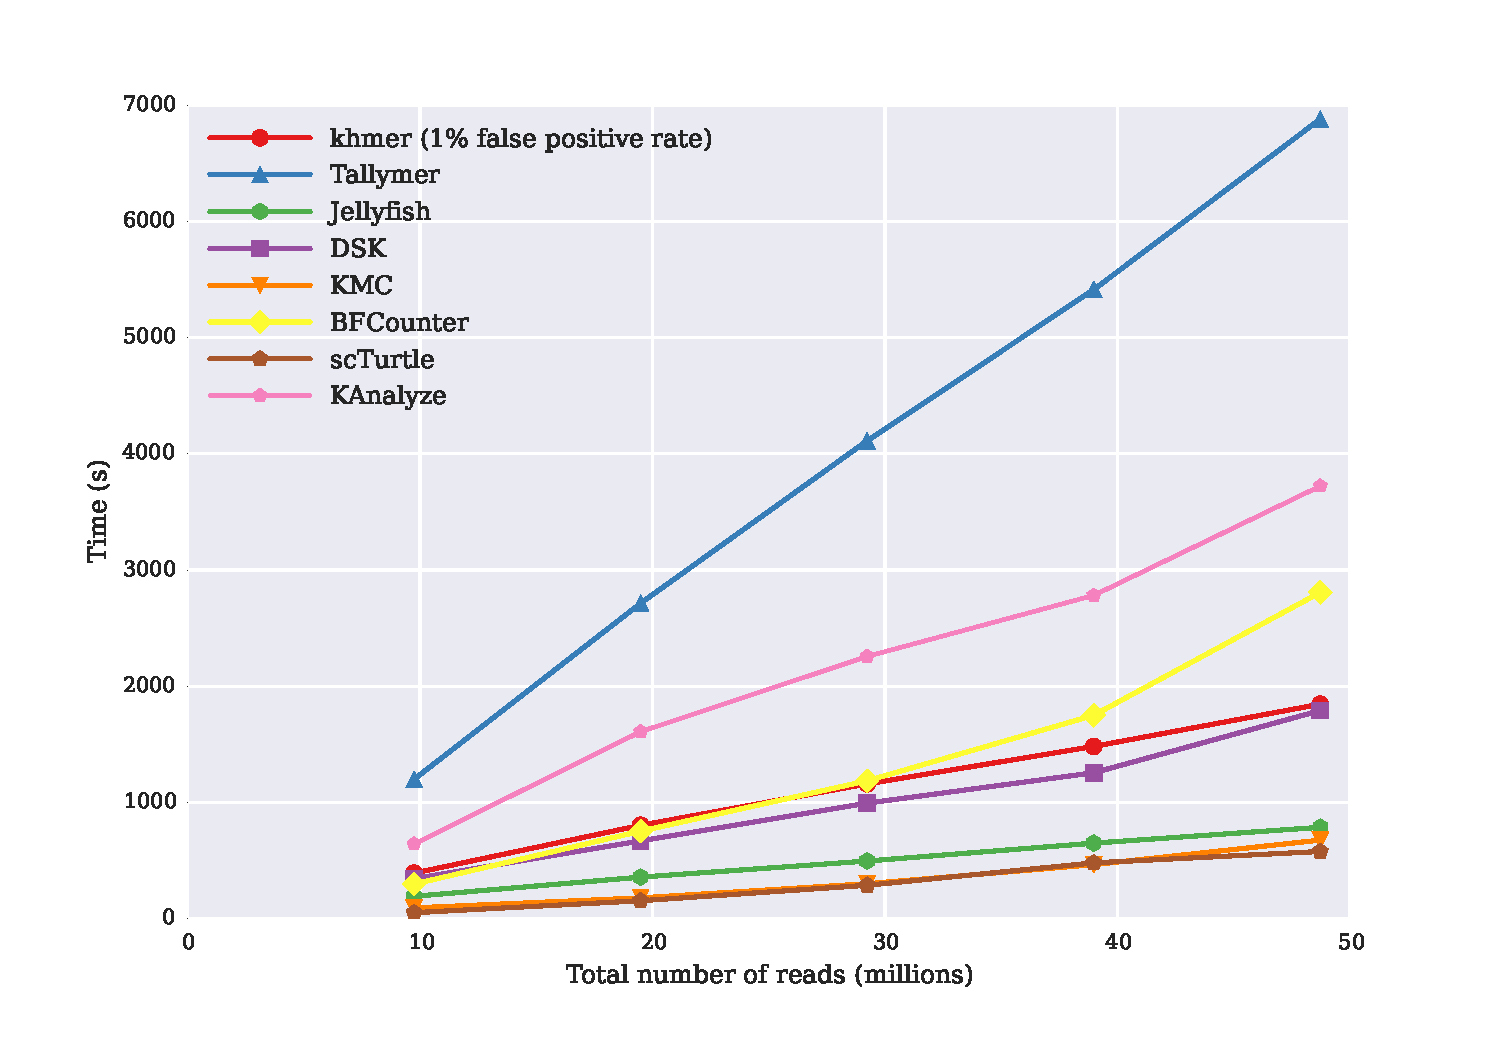
\includegraphics[width=5in]{./figure/figure1_time_benchmark}}

\caption{\bf Comparison of the time it takes for k-mer counting tools
  to calculate k-mer abundance histograms, with time (y axis, in
  seconds) against data set size (in number of reads, x axis).  
  All programs executed in time approximately linear with
  the number of input reads.}

\label{fig:cmp_time}
\end{figure}

\begin{figure}[!ht]
%\centerline{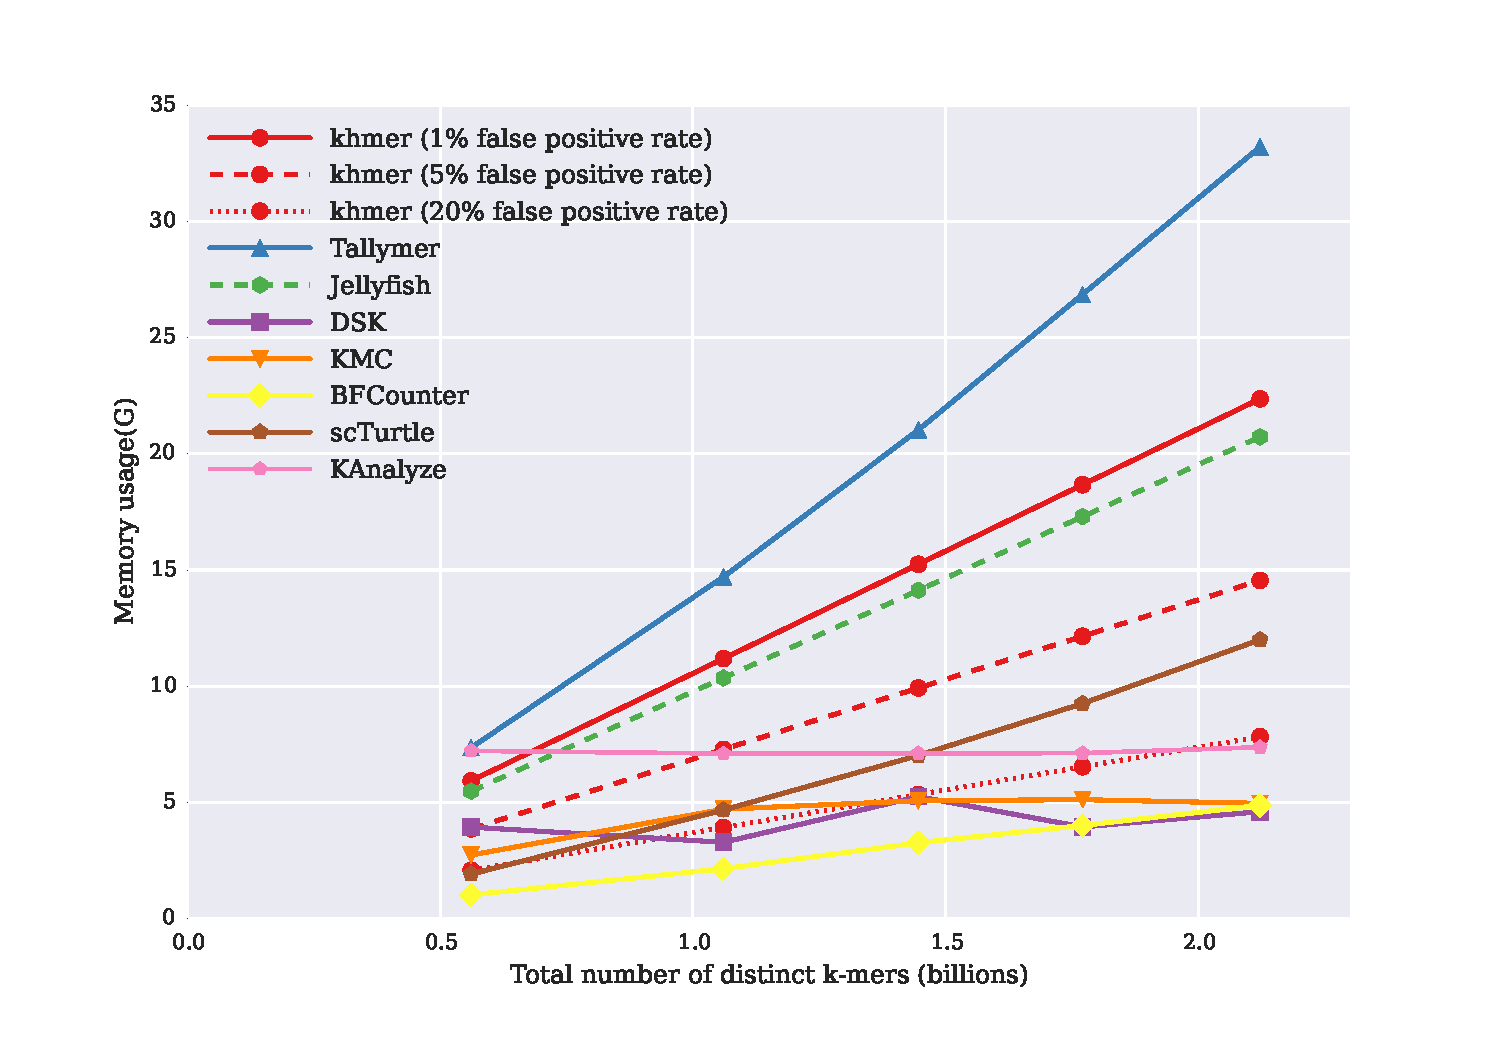
\includegraphics[width=5in]{./figure/figure2_memory_benchmark}}

\caption{\bf Memory usage of k-mer counting tools when calculating
  k-mer abundance histograms, with maximum resident program size (y
  axis, in GB) plotted against the total number of distinct k-mers in
  the data set (x axis, billions of k-mers). }

\label{fig:cmp_memory}
\end{figure}

\begin{figure}[!ht]
%\centerline{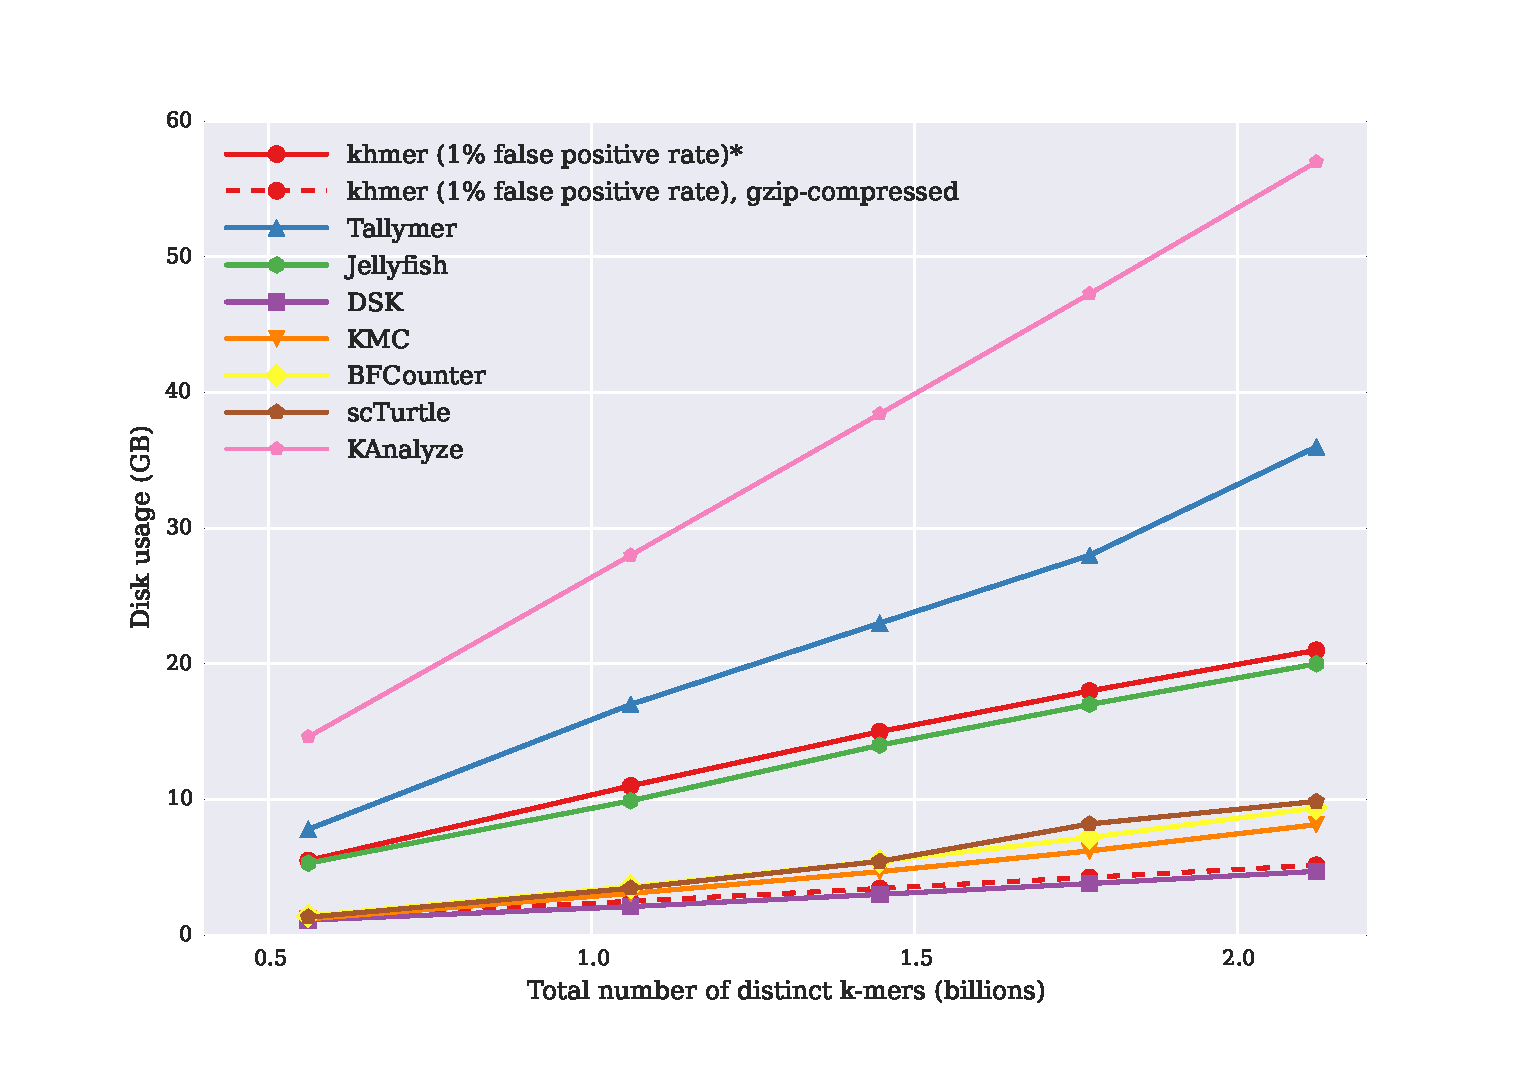
\includegraphics[width=5in]{./figure/figure3_disk_benchmark}}

\caption{\bf Disk storage usage of different k-mer counting tools to
  calculate k-mer abundance histograms in GB (y axis), plotted against
  the number of distinct k-mers in the data set (x axis).  $^*$Note
  that khmer does not use the disk during counting or retrieval,
  although its hash tables can be saved for reuse.}

\label{fig:cmp_disk}
\end{figure}

\begin{figure}[!ht]
%\centerline{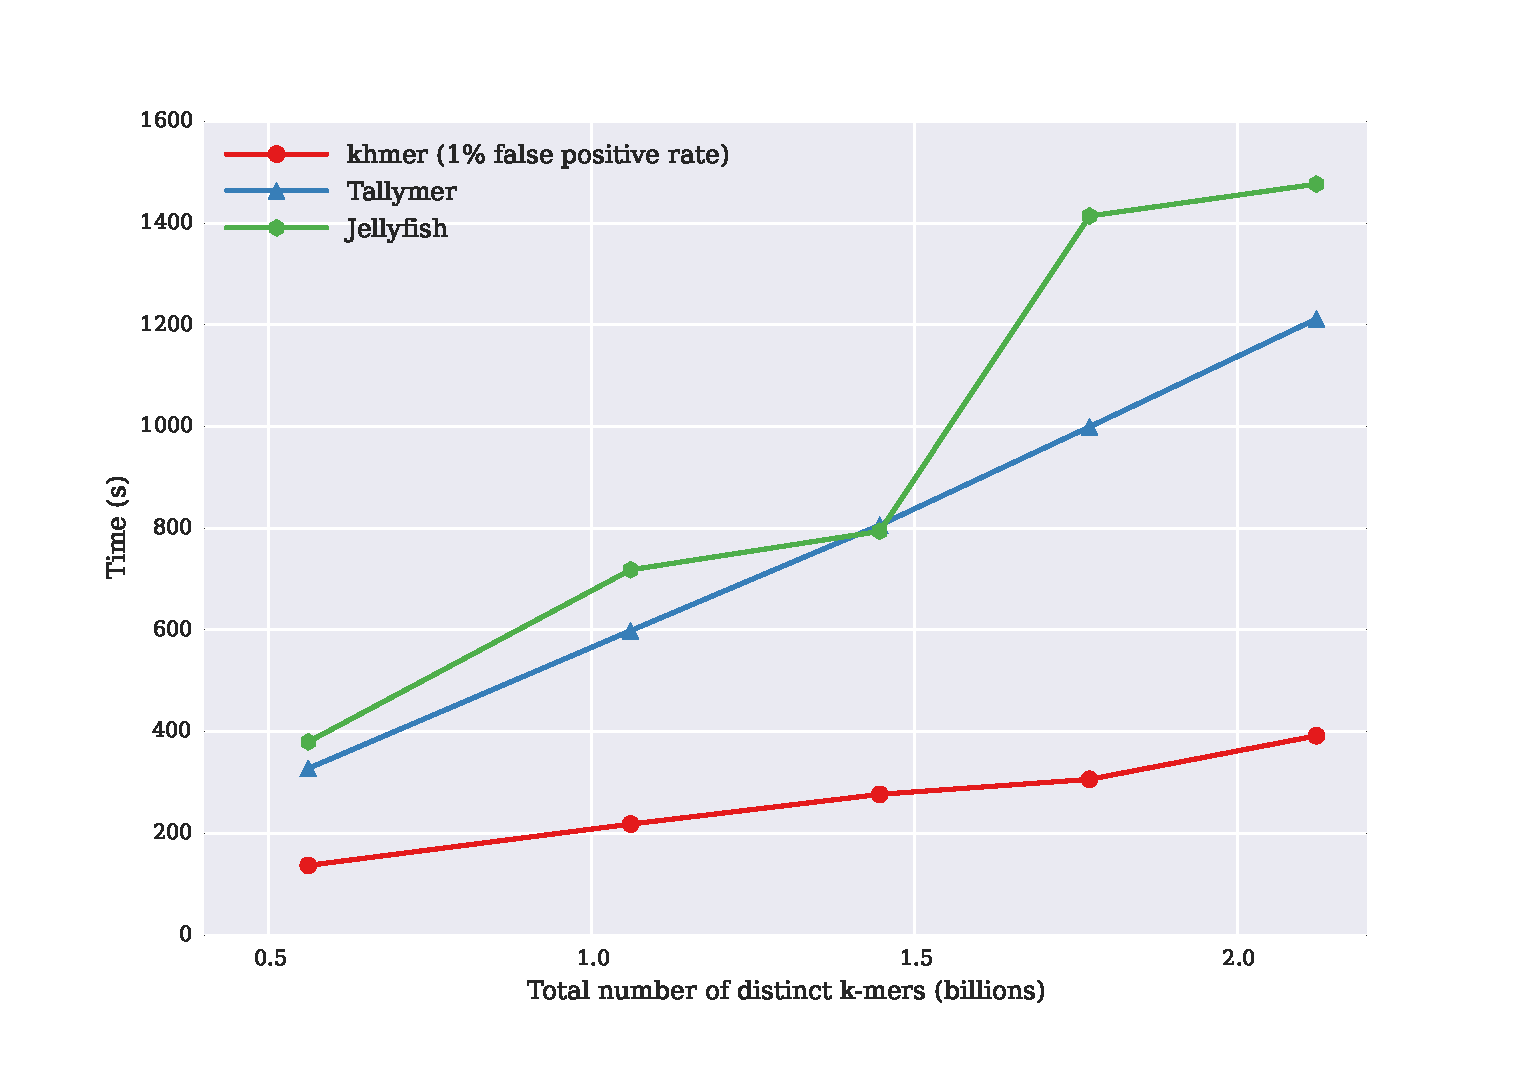
\includegraphics[width=5in]{./figure/figure4_count_benchmark}}
\caption{\bf Time for several k-mer counting tools to retrieve the
  counts of 9.7m randomly chosen k-mers (y axis), plotted against the
  number of distinct k-mers in the data set being queried (x axis).
  BFCounter, DSK, Turtle, KAnalyze, and KMC do not support this functionality.}
\label{fig:cmp_count}
\end{figure}

\begin{figure}[!ht]
%\centerline{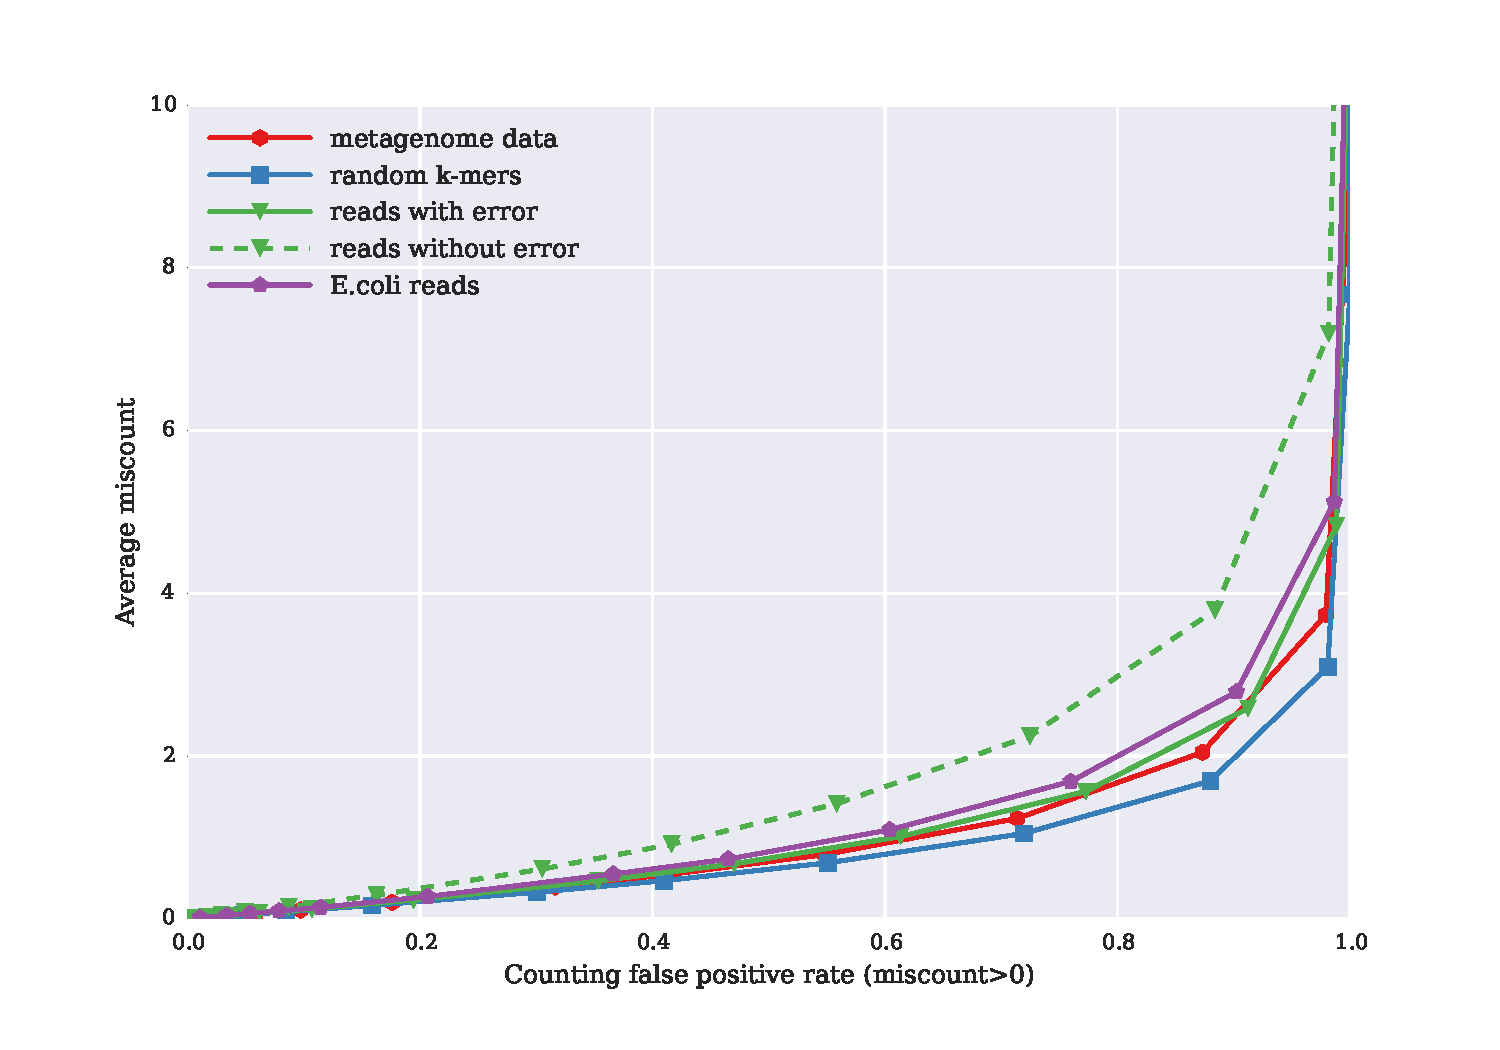
\includegraphics[width=5in]{./figure/figure5_average_offset_vs_fpr}}
\caption{\bf Relation between average miscount --- amount by which
the count for k-mers is incorrect --- on the y axis, plotted against
false positive rate (x axis), for five data sets.  The five data
sets were chosen to have the same total number of distinct k-mers: one
metagenome data set; a set of randomly generated k-mers; a set
of reads, chosen with 3x coverage and 1\% error, from a randomly generated
genome; a simulated set of error-free reads (3x) chosen from a randomly
generated genome and a set of {\em E. coli} reads.}
\label{fig:average_offset_vs_fpr}
\end{figure}

\begin{figure}[!ht]
%\centerline{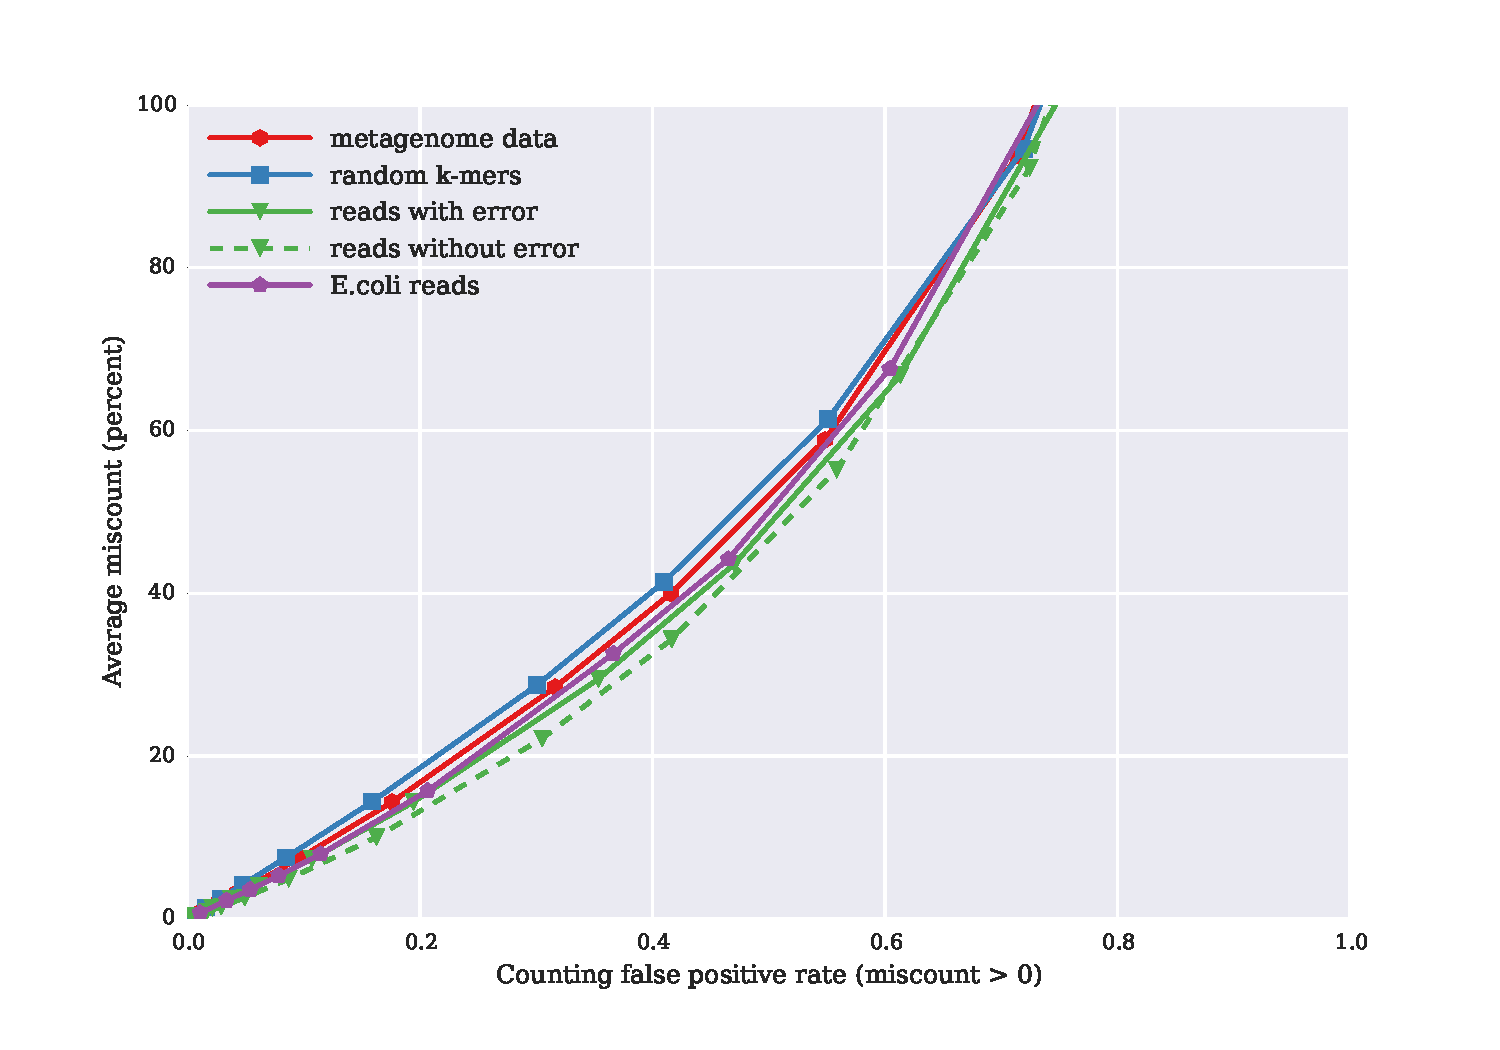
\includegraphics[width=5in]{./figure/figure6_percent_offset_vs_fpr}}
\caption{\bf Relation between percent miscount --- amount by which the
  count for k-mers is incorrect relative to its true count --- on the
  y axis, plotted against false positive rate (x axis), for five data
  sets.  The five data sets are the same as in Figure
  \ref{fig:average_offset_vs_fpr}.}
\label{fig:percent_offset_vs_fpr}
\end{figure}

\begin{figure}[!ht]
%\centerline{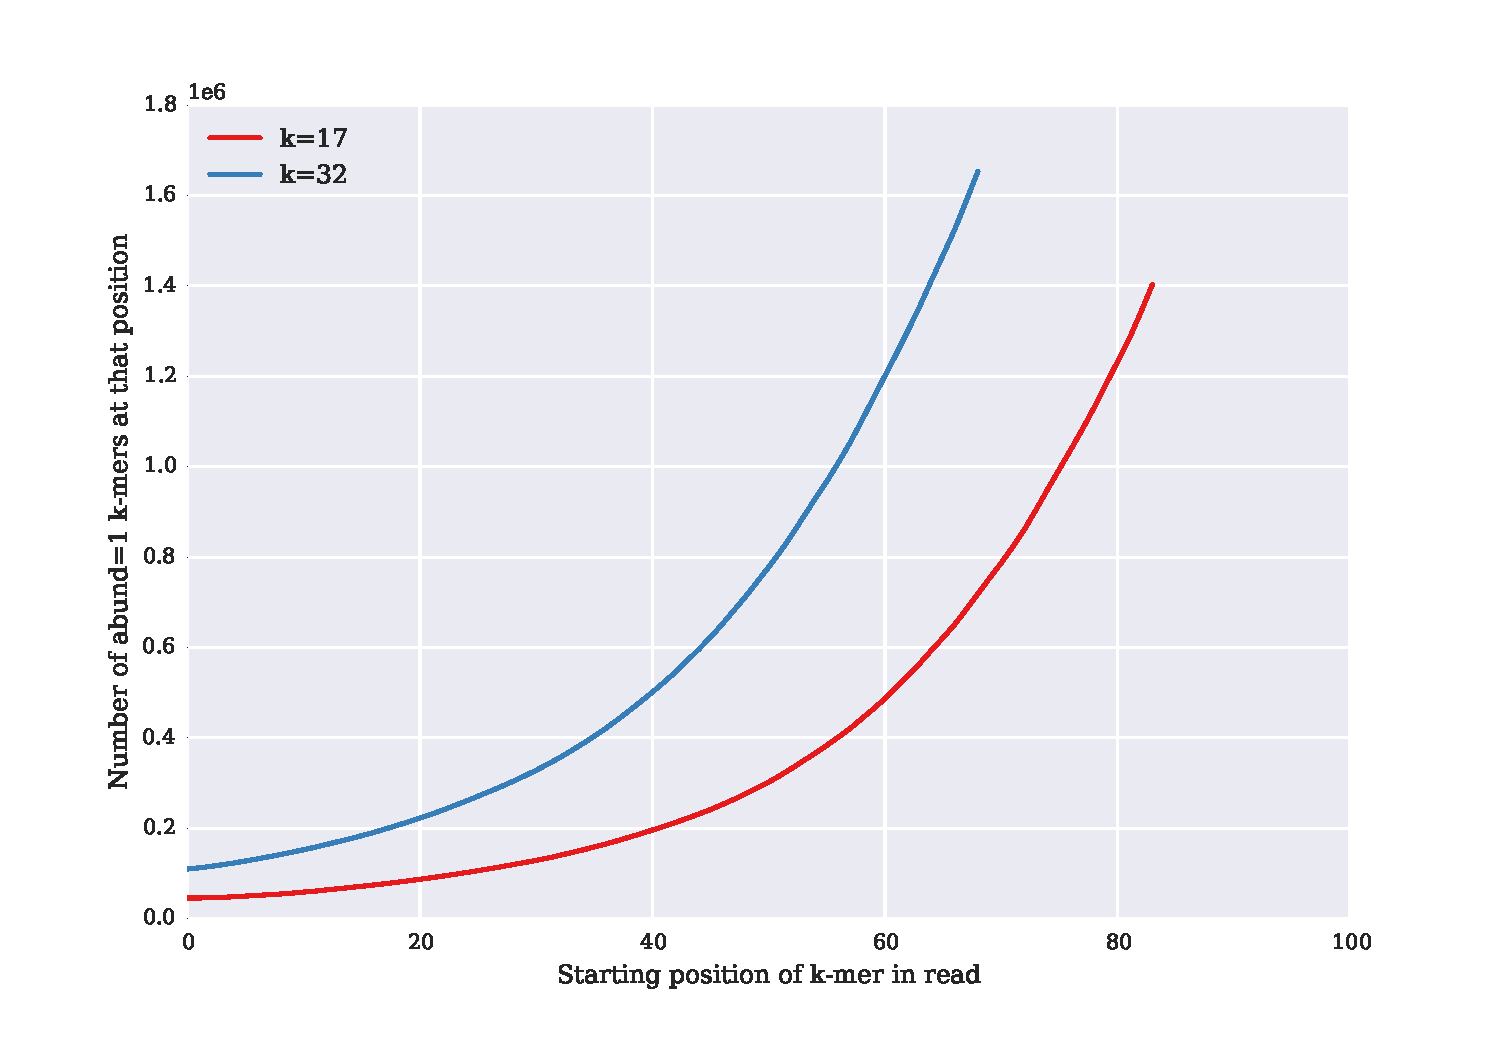
\includegraphics[width=5in]{./figure/figure7_perc_unique_pos}}
\caption{\bf Number of unique k-mers (y axis) by starting position
  within read (x axis) in an untrimmed {\em E. coli} 100-bp Illumina
  shotgun data set, for k=17 and k=32.  The increasing numbers of
  unique k-mers are a sign of the increasing sequencing error towards
  the 3' end of reads.  Note that there are only 69 starting positions
  for 32-mers in a 100 base read.}
\label{fig:perc_unique_pos}
\end{figure}

\clearpage
\section*{Tables}
%\begin{table}[!ht]
%\caption{
%\bf{Table title}}
%\begin{tabular}{|c|c|c|}
%table information
%\end{tabular}
%\begin{flushleft}Table caption
%\end{flushleft}
%\label{tab:label}
% \end{table}

% @CTB fix data set names/descr; caption; reference.
\begin{table}[!ht]
\caption{
\bf{Benchmark soil metagenome data sets for k-mer counting performance, taken from
\cite{Howe2012}.}}
\begin{tabular}{ |c | c |c| c|c| }
\hline
Data set & size of file (GB) & number of reads & number of distinct
k-mers & total number of k-mers \\
\hline
subset 1        & 1.90 &  9,744,399 &   561,178,082 &   630,207,985 \\
subset 2        & 2.17 & 19,488,798 & 1,060,354,144 & 1,259,079,821 \\
subset 3        & 3.14 & 29,233,197 & 1,445,923,389 & 1,771,614,378 \\
subset 4        & 4.05 & 38,977,596 & 1,770,589,216 & 2,227,756,662 \\
entire data set & 5.00 & 48,721,995 & 2,121,474,237 & 2,743,130,683 \\
\end{tabular}
\begin{flushleft}
\end{flushleft}
\label{table:datasets}
\end{table}

%%%%%%%%%%%%%%%%%%%%%%%

% These numbers are got by running these commands: (to be integrated in Makefile)

% to get number of distinct k-mers:
% python bloom_count.py ecoli_ref_head45000.fasta 12 100000000 4
% python bloom_count.py random_kmers_1M_3c.fa 12 100000000 4
% python bloom_count.py random_reads_1.67M_3c_0.03e.fa 12 100000000 4
% python bloom_count.py random_reads_2.54M_3c_0.00e.fa 12 100000000 4
% python bloom_count.py MH0001.trimmed.head176800.fa 12 100000000 4
% 
% to get number of total k-mers:
% number of reads x reads_length -12 + 1
% reads length = 44bp, except ecoli reads = 100 bp


\begin{table}[!ht]
\caption{
\bf{Data sets used for analyzing miscounts.}}
\begin{tabular}{ | p{5cm} | c | c | c |}
\hline
Data set & Size of data set file & Number of total k-mers & Number of distinct k-mers \\
\hline
Real metagenomics reads                                  & 7.01M  & 2,917,200  & 1,944,996 \\
\hline
Totally random reads with randomly generated k-mers      & 3.53M  & 2,250,006  & 1,973,059 \\
\hline
Simulated reads from simulated genome with error         & 5.92M  & 3,757,479  & 2,133,592 \\
\hline
Simulated reads from simulated genome without error      & 9.07M  & 5,714,973  & 1,989,644 \\
\hline
Real {\em E. coli} reads                                        & 4.85M  & 4,004,911  & 2,079,302 \\
\end{tabular}
\begin{flushleft}
\end{flushleft}
\label{table:random_data}
\end{table}



%%%%%%%%%%%%%%%%%%%%%%%

\begin{table}[!ht]
\caption{
\bf{Iterative low-memory k-mer trimming.  The results of trimming
  reads at unique (erroneous) k-mers from a 5m read {\em E. coli} data set (1.4 GB)
  in under 30 MB of RAM.  After each iteration, we measured the
  total number of distinct k-mers in the data set, the total number
  of unique (and likely erroneous) k-mers remaining, and the
  number of unique k-mers present at the 3' end of reads.}}
\begin{tabular}{ | c | c | c | c | c | c |}
\hline
 & FP rate & bases trimmed & distinct k-mers & unique k-mers & 
unique k-mers at 3' end \\
\hline
untrimmed                           &      -  &      - & 41.6m & 34.1m & 30.4\%  \\
khmer iteration 1                   & 80.0\%  & 13.5\% & 13.3m &  6.5m & 29.8\% \\
khmer iteration 2                   & 40.2\%  &  1.7\% &  7.6m & 909.9k & 12.3\% \\
khmer iteration 3                   & 25.4\%  &  0.3\% &  6.8m & 168.1k & 3.1\% \\
khmer iteration 4                   & 23.2\%  &  0.1\% &  6.7m &  35.8k & 0.7\% \\
khmer iteration 5                   & 22.8\%  &  0.0\% &  6.6m &   7.9k & 0.2\% \\
khmer iteration 6                   & 22.7\%  &  0.0\% &  6.6m &   1.9k & 0.0\% \\
filter by FASTX                     &      -  &  9.1\% & 26.6m & 20.3m & 26.3\% \\
filter by seqtk(default)            &      -  &  8.9\% & 17.7m & 12.1m & 12.3\% \\
filter by seqtk(-q 0.01)            &      -  & 15.4\% &  9.9m &  5.1m &  5.2\% \\
filter by seqtk(-b 3 -e 5)          &      -  &  8.0\% & 34.5m & 27.7m & 25.3\% \\
\end{tabular}
\begin{flushleft}
\end{flushleft}
\label{table:loop_trim}
\end{table}


%%%%%%%%%%%%%%%%%%

% data in pipeline/keep*.x.mg*.hist (true k-mers)
% data in pipeline/mg*.x.keep*.hist (total k-mers)
% data in pipeline/keep*.x.mg*.hist (true k-mers)
% @CTB address -2 issue
\begin{table}[!ht]
\caption{ \bf{Low-memory digital normalization. The results of
    digitally normalizing a 5m read {\em E. coli} data set (1.4 GB) to C=20
    with k=20 under several memory usage/false positive rates.  The
    false positive rate (column 1) is empirically determined.  We
    measured reads remaining, number of ``true'' k-mers missing from
    the data at each step, and the number of total k-mers remaining.
    Note: at high false positive rates, reads are erroneously removed due to
    inflation of k-mer counts.}}
\begin{tabular}{ | c | c | c | c | c | c | c |}
\hline
memory   & FP rate & retained reads & retained reads \% & true k-mers missing & total k-mers \\
\hline
before diginorm   &  -      & 5,000,000   & 100.0\%    & 170  &  41.6m \\
2400 MB           &   0.0\% & 1,656,518   &  33.0\%    & 172  &  28.1m \\
240 MB            &   2.8\% & 1,655,988   &  33.0\%    & 172  &  28.1m \\
120 MB            &  18.0\% & 1,652,273   &  33.0\%    & 172  &  28.1m \\
60 MB             &  59.1\% & 1,633,182   &  32.0\%    & 172  &  27.9m \\
40 MB             &  83.2\% & 1,602,437   &  32.0\%    & 172  &  27.6m \\
20 MB             &  98.8\% & 1,460,936   &  29.0\%    & 172  &  25.7m \\
10 MB             & 100.0\% & 1,076,958   &  21.0\%    & 185  &  20.9m \\
\end{tabular}
\begin{flushleft}
\end{flushleft}
\label{table:loop_norm}
\end{table}

%%%%%%%%%%%%%%%%%%%%%%%%%%%

% data in *.cover
\begin{table}[!ht]
\caption{
\bf{{\em E. coli} genome assembly after low-memory digital normalization.
  A comparison of assembling reads digitally normalized with low memory/high
  false positive rates.  The reads were digitally normalized to 
  C=20 (see
  \cite{Brown2012} for more information) and were assembled using Velvet.
  We measured total length of assembly,
  as well as percent of true MG1655 genome covered by the assembly using QUAST.}}
\begin{tabular}{ | c | c | c | c | c | c |}
\hline
memory   & FP rate & N contigs & total length(bases) & \% of true genome covered \\
\hline
before diginorm  &-   & 106 & 4,546,051 & 97.84\% \\
    2400 MB  &  0.0\% & 617 & 4,549,235 & 98.05\% \\
     240 MB  &  2.8\% &  87 & 4,549,253 & 98.04\% \\
     120 MB  & 18.0\% &  86 & 4,549,335 & 98.04\% \\
      60 MB  & 59.1\% &  90 & 4,548,619 & 98.03\% \\
      40 MB  & 83.2\% &  89 & 4,550,599 & 98.11\% \\
      20 MB  & 98.8\% &  85 & 4,550,014 & 98.04\% \\
      10 MB  &100.0\% &  97 & 4,545,871 & 97.97\% \\
\end{tabular}
\begin{flushleft}
\end{flushleft}
\label{table:assembly}
\end{table}
% @CTB be sure to explain the tables well!
% @CTB do we talk about how efficiently fp rate drops with incr memory?
% @CTB make point that diginorm/first step is hard.
% @CTB KMC


\chapter{diginorm: need rewriting, plan: only keep the materilas that are more relevant to IGS }

\section{Introduction}

The ongoing improvements in DNA sequencing technologies have led to a
new problem: how do we analyze the resulting large sequence data sets
quickly and efficiently? These data sets contain millions to billions
of short reads with high error rates and substantial sampling
biases \cite{pubmed19997069}.  The vast quantities of deep sequencing
data produced by these new sequencing technologies are driving
computational biology to extend and adapt previous approaches to
sequence analysis.  In particular, the widespread use of deep shotgun
sequencing on previously unsequenced genomes, transcriptomes, and
metagenomes, has resulted in the development of several new approaches
to {\em de novo} sequence assembly \cite{pubmed20211242}.

There are two basic challenges in analyzing short-read sequences from
shotgun sequencing. First, deep sequencing is needed for complete
sampling. This is because shotgun sequencing samples randomly from a
population of molecules; this sampling is biased by sample content and
sample preparation, requiring even deeper sequencing. A human genome
may require 100x coverage or more for near-complete sampling, leading
to shotgun data sets 300 GB or larger in size\cite{pubmed21187386}.
Since the lowest abundance molecule determines the depth of coverage
required for complete sampling, transcriptomes and metagenomes
containing rare population elements can also require similarly
deep sequencing.

The second challenge to analyzing short-read shotgun sequencing is the
high error rate.  For example, the Illumina GAII sequencer has a 1-2\% error
rate, yielding an average of one base error in every 100 bp of data
\cite{pubmed19997069}.  The total number of errors grows linearly with
the amount of data generated, so these errors usually dominate
novelty in large data sets \cite{pubmed21245053}.  Tracking this
novelty and resolving errors is computationally expensive.

These large data sets and high error rates combine to provide a third
challenge: it is now straightforward to generate data sets that cannot
easily be analyzed \cite{pubmed21867570}.  While hardware approaches
to scaling existing algorithms are emerging, sequencing capacity
continues to grow faster than computational capacity
\cite{pubmed20441614}.  Therefore, new algorithmic approaches to
analysis are needed.

Many new algorithms and tools have been developed to tackle large and
error-prone short-read shotgun data sets. A new class of alignment
tools, most relying on the Burrows-Wheeler transform, has been created
specifically to do ultra-fast short-read alignment to reference
sequence \cite{pubmed19430453}.  In cases where a reference sequence
does not exist and must be assembled {\em de novo} from the sequence
data, a number of new assemblers have been written, including ABySS,
Velvet, SOAPdenovo, ALLPATHS, SGA, and Cortex
\cite{pubmed19251739,pubmed18349386,pubmed20511140,pubmed21187386,pubmed22156294,cortex}.
These assemblers rely on theoretical advances to store and assemble
large amounts of data \cite{pubmed22068540,pubmed20529929}.  As
short-read sequencing has been applied to single cell genomes,
transcriptomes, and metagenomes, yet another generation of assemblers
has emerged to handle reads from abundance-skewed populations of
molecules; these tools, including Trinity, Oases, MetaVelvet,
Meta-IDBA, and Velvet-SC, adopt local models of sequence coverage to
help build assemblies
\cite{pubmed21572440,pubmed22368243,metavelvet,pubmed21685107,pubmed21926975}.
In addition, several ad hoc strategies have also been applied to reduce
variation in sequence content from whole-genome amplification
\cite{pubmed19724646,pubmed22028825}.
Because these tools all rely on k-mer approaches and require exact
matches to construct overlaps between sequences, their performance is
very sensitive to the number of errors present in the underlying data.
This sensitivity to errors has led to the development of a number of
error removal and correction approaches that preprocess data prior to
assembly or mapping
\cite{pubmed21685062,pubmed15059830,pubmed21114842}.

%One approach to error correction involves finding low-abundance
%fixed-length words, or k-mers, and treating them as likely errors;
%these errors can then be ``corrected'' by changing them to similar
%k-mers that are in high abundance \cite{pubmed21114842}.  This
%approach requires two complete iterations across the data set: one
%iteration to collect abundance spectra, and a second to perform the
%trimming or correction.  For extremely large data sets, this is a
%significant problem: the ``noise'' from sequencing errors drives a
%supra-linear increase in the number of k-mers, so as data set size
%increases, the computation and memory needed to track k-mers increases
%dramatically \cite{pubmed21245053}.

Below, we introduce ``digital normalization'', a single-pass algorithm
for elimination of redundant reads in data sets.  Critically, no
reference sequence is needed to apply digital normalization.  Digital
normalization is inspired by experimental normalization techniques
developed for cDNA library preparation, in which hybridization
kinetics are exploited to reduce the copy number of abundant
transcripts prior to sequencing\cite{pubmed8889548,pubmed7937745}.
{\em Digital} normalization works after sequencing data has been
generated, progressively removing high-coverage reads from shotgun
data sets.  This normalizes average coverage to a specified value,
reducing sampling variation while removing reads, and also removing
the many errors contained {\em within} those reads.  This data and
error reduction results in dramatically decreased computational
requirements for {\em de novo} assembly.  Moreover, unlike experimental
normalization where abundance information is removed prior to sequencing,
in digital normalization this information can be recovered from the
unnormalized reads.

% @@ where do I mention prior approaches?

%The digital normalization algorithm is inspired by experimental
%normalization techniques developed for cDNA library preparation.  In
%experimental normalization, hybridization kinetics are exploited to
%reduce the copy number of highly abundant transcripts, ``normalizing''
%or evening out the abundance distribution so that shotgun cloning and
%sequencing recover low-abundance molecules as well as high-abundance
%molecules \cite{pubmed8889548,pubmed7937745}.  {\em Digital}
%normalization was initially designed to deal with reads from
%abundance-skewed samples such as single-cell amplified genomic DNA,
%transcriptomes, and metagenomes
%\cite{pubmed16732271,pubmed19015660,pubmed16304596}.

%Digital normalization systematically removes high-coverage reads from
%data sets.  Errors contained in these discarded reads do not then
%accumulate in the normalized data set, and we see a substantial
%reduction in the total number of errors.

We present here a fixed-memory implementation of digital normalization
that operates in time linear with the size of the input data.  We then
demonstrate its effectiveness for reducing compute requirements for
{\em de novo} assembly on several real data sets.  These data sets
include {\em E. coli} genomic data, data from two single-cell
MD-amplified microbial genomes, and yeast and mouse mRNAseq.

% Results and Discussion can be combined.
\section{Results}

\subsection{Estimating sequencing depth without a reference assembly}

Short-read assembly requires deep sequencing to systematically sample
the source genome, because shotgun sequencing is subject to both
random sampling variation and systematic sequencing biases.  For
example, 100x sampling of a human genome is required for recovery of
90\% or more of the genome in contigs $>$ 1kb \cite{pubmed21187386}.
In principle much of this high-coverage data is redundant and could be
eliminated without consequence to the final assembly, but determining
which reads to eliminate requires a per-read estimate of coverage.
Traditional approaches estimate coverage by mapping reads to an
assembly.  This presents a chicken-and-egg problem: to
determine which regions are oversampled, we must already have an
assembly!

We may calculate a {\em reference-free} estimate of genome coverage by
looking at the k-mer abundance distribution within individual reads.
First, observe that k-mers, DNA words of a fixed length $k$, tend to
have similar abundances within a read: this is a well-known property
of k-mers that stems from each read originating from a single source
molecule of DNA.  The more times a region is sequenced, the higher the
abundance of k-mers from that region would be.  In the absence of
errors, average k-mer abundance could be used as an estimate of the
depth of coverage for a particular read (Figure \ref{fig:rankabund},
``no errors'' line).  However, when reads contain random substitution
or indel errors from sequencing, the k-mers overlapping these errors
will be of lower abundance; this feature is often used in k-mer based
error correction approaches \cite{pubmed21114842}.  For example, a
single substitution will introduce $k$ low-abundance k-mers within a
read.  (Figure \ref{fig:rankabund}, ``single substitution error''
line).  However, for small $k$ and reads of length $L$ where $L >
3k-1$, a single substitution error will not skew the {\em median}
k-mer abundance.  Only when multiple substitution errors are found in
a single read will the median k-mer abundance be affected (Figure
\ref{fig:rankabund}, ``multiple substitution errors'').

Using a fixed-memory CountMin Sketch data structure to count k-mers
(see Methods and \cite{countminsketch}), we find that median k-mer
abundance correlates well with mapping-based coverage for artificial
and real genomic data sets.  There is a strong correlation between
median k-mer abundance and mapping-based coverage both for simulated
100-base reads generated with 1\% error from a 400kb artificial genome
sequence ($r^2 = 0.79$; also see Figure \ref{fig:random}a), as well as
for real short-read data from {\em E. coli} ($r^2 = 0.80$, also see
Figure \ref{fig:random}b).  This correlation also holds for simulated
and real mRNAseq data: for simulated transcriptome data, $r^2 = 0.93$
(Figure \ref{fig:transcripts}a), while for real mouse transcriptome
data, $r^2 = 0.90$ (Figure \ref{fig:transcripts}b).
Thus the median k-mer abundance of a read correlates
well with mapping-based estimates of read coverage.

%We next investigate ways of using this estimator to remove highly
%sampled regions prior to {\em de novo} assembly.

\subsection{Eliminating redundant reads reduces variation in sequencing depth}

Deeply sequenced genomes contain many highly covered loci.  For
example, in a human genome sequenced to 100x average coverage, we would
expect 50\% or more of the reads to have a coverage greater than 100.
In practice, we need many fewer of these reads to assemble
the source locus.

Using the median k-mer abundance estimator discussed above, we can examine each read
in the data set progressively to determine if it is high coverage.  At
the beginning of a shotgun data set, we would expect many reads to be
entirely novel and have a low estimated coverage.  As we proceed
through the data set, however, average coverage will increase and many
reads will be from loci that we have already sampled sufficiently.

Suppose we choose a coverage threshold $C$ past which we no longer
wish to collect reads. If we only keep reads whose estimated coverage
is less than $C$, and discard the rest, we will reduce the average
coverage of the data set to $C$.  This procedure is
algorithmically straightforward to execute: we examine each read's
estimated coverage, and retain only those whose coverage is less than $C$.
The following pseudocode provides one approach:
\begin{verbatim}
   for read in dataset:
      if estimated_coverage(read) < C:
         accept(read)
      else:
         discard(read)
\end{verbatim}
\noindent
where accepted reads contribute to the $\tt estimated\_coverage$
function.  Note that for any data set with an average coverage $> 2C$,
this has the effect of discarding the majority of reads.  Critically,
low-coverage reads, especially reads from undersampled regions, will
always be retained.

The net effect of this procedure, which we call digital normalization,
is to normalize the coverage distribution of data sets.  In Figure
\ref{fig:coverage}a, we display the estimated coverage of an {\em
  E. coli} genomic data set, a {\em S. aureus} single-cell
MD-amplified data set, and an MD-amplified data set from an uncultured
{\em Deltaproteobacteria}, calculated by mapping reads to the known or
assembled reference genomes (see \cite{pubmed21926975} for the data
source).  The wide variation in coverage for the two MDA data sets is
due to the amplification procedure \cite{pubmed17487184}.  After
normalizing to a k-mer coverage of 20, the high coverage loci are
systematically shifted to an average mapping coverage of 26, while
lower-coverage loci remain at their previous coverage.  This smooths
out coverage of the overall data set.

At what rate are sequences retained?  For the {\em E. coli} data set,
Figure \ref{fig:accumulate} shows the fraction of sequences retained
by digital normalization as a function of the total number of reads
examined when normalizing to C=20 at k=20.  There is a clear
saturation effect showing that as more reads are examined, a smaller
fraction of reads is retained; by 5m reads, approximately 50-100x
coverage of {\em E. coli}, under 30\% of new reads are kept.  This
demonstrates that as expected, only a small amount of novelty (in
the form of either new information, or the systematic accumulation of
errors) is being observed with increasing sequencing depth.

\subsection{Digital normalization retains information while discarding
both data and errors}

The 1-2\% per-base error rate of next-generation sequencers
dramatically affect the total number of k-mers.  For example, in the
simulated genomic data of 200x, a 1\% error rate leads to
approximately 20 new k-mers for each error, yielding 20-fold more
k-mers in the reads than are truly present in the genome (Table 1, row
1).  This in turn dramatically increases the memory requirements for
tracking and correcting k-mers \cite{pubmed21245053}.  This is a
well-known problem with de Bruijn graph approaches, in which erroneous
nodes or edges quickly come to dominate deep sequencing data sets.

When we perform digital normalization on such a data set, we eliminate
the vast majority of these k-mers (Table \ref{tab:normC20}, row 1).
This is because we are accepting or rejecting entire reads; in
going from 200x random coverage to 20x systematic coverage, we
discard 80\% of the reads containing 62\% of the errors (Table
\ref{tab:normC20}, row 1).  For reads taken from a skewed abundance
distribution, such as with MDA or mRNAseq, we similarly discard many
reads, and hence many errors (Table \ref{tab:normC20}, row 2).  In
fact, in most cases the process of sequencing fails to recover
more true k-mers (Table \ref{tab:normC20}, middle column, parentheses) than
digital
normalization discards (Table \ref{tab:normC20}, fourth column, parentheses).

The net effect of digital normalization is to retain nearly all {\em
  real} k-mers, while discarding the majority of erroneous k-mers --
in other words, digital normalization is discarding {\em data} but not
{\em information}.  This rather dramatic elimination of erroneous
k-mers is a consequence of the high error rate present in reads: with
a 1\% per-base substitution error rate, each 100-bp read will have an
average of one substitution error. Each of these substitution errors
will introduce up to $k$ erroneous k-mers.  Thus, for each read we
discard as redundant, we also eliminate an average of $k$ erroneous
k-mers.

We may further eliminate erroneous k-mers by removing k-mers that are
rare across the data set; these rare k-mers tend to result from
substitution or indel errors \cite{pubmed21114842}.  We do this by
first counting all the k-mers in the accepted reads during digital
normalization.  We then execute a second pass across the accepted
reads in which we eliminate the 3' ends of reads at low-abundance
k-mers.  Following this error reduction pass, we execute a
second round of digital normalization (a third pass across the data
set) that further eliminates redundant data.  This three-pass protocol
eliminates additional errors and results in a further decrease in data
set size, at the cost of very few real k-mers in genomic data sets
(Table \ref{tab:normC5}).

Why use this three-pass protocol rather than simply normalizing to the
lowest desired coverage in the first pass?  We find that removing
low-abundance k-mers after a single normalization pass to $C \approx
5$ removes many more {\em real} k-mers, because there will be many
regions in the genome that by chance have yielded 5 reads with errors
in them. If these erroneous k-mers are removed in the abundance-trimming step,
coverage of the corresponding regions is eliminated.  By normalizing
to a higher coverage of 20, removing errors, and only then reducing
coverage to 5, digital normalization can retain accurate reads for most
regions.  Note that this three-pass protocol is not considerably more
computationally expensive than the single-pass protocol: the first
pass discards the majority of data and errors, so later passes are
less time and memory intensive than the first pass.

Interestingly, this three-pass protocol removed many more real k-mers
from the simulated mRNAseq data than from the simulated genome -- 351
of 48,100 (0.7\%) real k-mers are lost from the mRNAseq, vs 4 of
399,981 lost (.000001\%) from the genome (Table \ref{tab:normC5}).
While still only a tiny fraction of the total number of real k-mers,
the difference is striking -- the simulated mRNAseq sample loses k-mers
at almost 1000-fold the rate of the simulated genomic sample.  Upon
further investigation, all but one of the lost k-mers were located
within 20 bases of the ends of the source sequences; see Figure
\ref{fig:endloss}.  This is because digital normalization cannot
distinguish between erroneous k-mers and k-mers that are undersampled
due to edge effects.  In the case of the simulated genome, which was
generated as one large chromosome, the effect is negligible, but the
simulated transcriptome was generated as 100 transcripts of length
500.  This added 99 end sequences over the genomic simulation, which
in turn led to many more lost k-mers.

While the three-pass protocol is effective at removing erroneous
k-mers, for some samples it may be too stringent.  For example, the
mouse mRNAseq data set contains only 100m reads, which may not be
enough to thoroughly sample the rarest molecules; in this case the
abundance trimming would remove real k-mers as well as erroneous k-mers.
Therefore we used the single-pass digital normalization
for the yeast and mouse transcriptomes.  For these two samples we can
also see that the first-pass digital normalization is extremely effective,
eliminating essentially all of the erroneous k-mers (Table \ref{tab:normC20},
rows 4 and 5.)

\subsection{Digital normalization scales assembly of microbial genomes}

We applied the three-pass digital normalization and error trimming
protocol to three real data sets from Chitsaz et al (2011)
\cite{pubmed21926975}.  The first pass of digital normalization was
performed in 1gb of memory and took about 1 min per million reads.
For all three samples, the number of reads remaining after digital
normalization was reduced by at least 30-fold, while the memory and
time requirements were reduced 10-100x.

%@@(For benchmarking, we used a
%more recent version of Velvet rather than Velvet-SC, because
%optimizations have been added to Velvet since the Velvet-SC fork.)

Despite this dramatic reduction in data set size and computational
requirements for assembly, both the {\em E. coli} and {\em S. aureus}
assemblies overlapped with the known reference sequence by more than
98\%.  This confirms that little or no information was lost during
the process of digital normalization; moreover, it appears that
digital normalization does not significantly affect the assembly results.
(Note that we did not perform scaffolding, since the digital
normalization algorithm does not take into account paired-end
sequences, and could mislead scaffolding approaches.  Therefore, these
results cannot directly be compared to those in Chitsaz et al. (2011)
\cite{pubmed21926975}.)

The {\em Deltaproteobacteria} sequence also assembled well, with
98.8\% sequence overlap with the results from Chitsaz et al.
Interestingly, only 30kb of the sequence assembled with Velvet-SC in
Chitsaz et al. (2011) was missing, while an additional 360kb of
sequence was assembled only in the normalized samples.  Of the 30kb of
missing sequence, only 10\% matched via TBLASTX to a nearby {\em
  Deltaproteobacteria} assembly, while more than 40\% of the
additional 360kb matched to the same {\em Deltaproteobacteria} sample.
Therefore these additional contigs likely represents real
sequence, suggesting that digital normalization is competitive with
Velvet-SC in terms of sensitivity.

%% @@ better assembly?

% @ tables or anything?

\subsection{Digital normalization scales assembly of transcriptomes}

We next applied single-pass digital normalization to published yeast
and mouse mRNAseq data sets, reducing them to 20x coverage at k=20
\cite{pubmed21572440}.  Digital normalization on these samples used
8gb of memory and took about 1 min per million reads.  We then
assembled both the original and normalized sequence reads with Oases
and Trinity, two {\em de novo} transcriptome assemblers (Table
\ref{tab:dntrans}) \cite{pubmed22368243,pubmed21572440}.
%  (Note that
%due to differing execution parameters, the Oases runtimes cannot be
%directly compared to the Trinity runtimes.)

For both assemblers the computational resources necessary to complete
an assembly were reduced (Table \ref{tab:dntrans}), but normalization
had different effects on performance for the different samples.  On the
yeast data set, time and memory requirements were reduced
significantly, as for Oases running on mouse.  However, while
Trinity's runtime decreased by a factor of three on the normalized
mouse data set, the memory requirements did not decrease
significantly.  This may be because the mouse transcriptome is 5-6
times larger than the yeast transcriptome, and so the mouse mRNAseq
is lower coverage overall; in this case we would expect fewer
errors to be removed by digital normalization.

The resulting assemblies differed in summary statistics (Table
\ref{tab:dntrans0}).  For both yeast and mouse, Oases lost 5-10\% of
total transcripts and total bases when assembling the normalized data.  However, Trinity {\em gained}
transcripts when assembling the normalized yeast and mouse data,
gaining about 1\% of total bases on yeast and losing about 1\%
of total bases in mouse.  Using a local-alignment-based overlap
analysis (see Methods) we found little difference in sequence
content between the pre- and post- normalization assemblies: for
example, the normalized Oases assembly had a 98.5\% overlap with the
unnormalized Oases assembly, while the normalized Trinity assembly had
a 97\% overlap with the unnormalized Trinity assembly.

To further investigate the differences between transcriptome
assemblies caused by digital normalization, we looked at the
sensitivity with which long transcripts were recovered
post-normalization.  When comparing the normalized assembly to the
unnormalized assembly in yeast, Trinity lost only 3\% of the sequence
content in transcripts greater than 300 bases, but 10\% of the
sequence content in transcripts greater than 1000 bases.  However,
Oases lost less than 0.7\% of sequence content at 300 and
1000 bases.  In mouse, we see the same pattern.
This suggests that the change in summary statistics for
Trinity is caused by fragmentation of long transcripts into shorter
transcripts, while the difference for Oases is caused by loss of
splice variants.  Indeed, this
loss of splice variants should be expected, as there are many low-prevalence splice
variants present in deep sequencing data \cite{pubmed21151575}.
Interestingly, in yeast we recover {\em more} transcripts after
digital normalization; these transcripts appear to be additional splice
variants.

% @table of splice foo?

The difference between Oases and Trinity results show that Trinity is
more sensitive to digital normalization than Oases: digital
normalization seems to cause Trinity to fragment long transcripts.
Why?  One potential issue is that Trinity only permits k=26 for
assembly, while normalization was performed at k=20; digital
normalization may be removing 26-mers that are important for Trinity's
path finding algorithm.  Alternatively, Trinity may be more sensitive
than Oases to the change in coverage caused by digital normalization.
Regardless, the strong performance of Oases on digitally normalized
samples, as well as the high retention of k-mers (Table \ref{tab:normC20})
suggests that the primary sequence content for the transcriptome remains
present in the normalized reads, although it is recovered with different
effectiveness by the two assemblers.

\section{Discussion}

\subsection{Digital normalization dramatically scales {\em de novo} assembly}

The results from applying digital normalization to read data sets
prior to {\em de novo} assembly are extremely good: digital
normalization reduces the computational requirements (time and memory)
for assembly considerably, without substantially affecting the
assembly results.  It does this in two ways: first, by removing
the majority of reads without significantly affecting the true k-mer
content of the data set. Second, by eliminating these reads,
digital normalization also eliminates sequencing errors contained
within those reads, which otherwise would add significantly to memory
usage in assembly \cite{pubmed21245053}.

Digital normalization also lowers computational requirements by
eliminating most repetitive sequence in the data set.
Compression-based approaches to graph storage have demonstrated that
compressing repetitive sequence also effectively reduces memory and
compute requirements \cite{pubmed22139935,pubmed22156294}.  Note
however that {\em eliminating} many repeats may also have its
negatives (discussed below).

Digital normalization should be an effective preprocessing approach
for most assemblers.  In particular, the de Bruijn graph approach used
in many modern assemblers relies on k-mer content, which is almost
entirely preserved by digital normalization (see Tables \ref{tab:normC20}
and \ref{tab:normC5}) \cite{pubmed20211242}.

%First, digital normalization removes the majority of reads without
%significantly affecting the true k-mer content of the data set.  This
%reduces the time required to load the data.  Moreover, digital
%normalization provides a simple principled way to combine data from
%multiple samples to maximize the sensitivity of assembly.  This is
%similar to approaches such as Fulcrum, which also losslessly remove
%redundant data, albeit less efficiently \cite{pubmed22419786}.

%Second, digital normalization eliminates sequencing errors contained
%in the removed reads.  These sequencing errors would add significantly
%to memory usage for de Bruijn graph assemblers .
%This is one reason why error filtering or correction is a strongly
%recommended step prior to genome assembly, and digital normalization
%is therefore an efficient approach to error removal.

%Third, by normalizing the read coverage, digital normalization
%removes biases in coverage, including those due to sampling bias and
%underlying non-uniform molecule distributions.  This allows
%single-genome assemblers such as Velvet to be applied to samples with
%skewed source distributions such as mRNAseq and MDA-amplified genomes,
%as well as metagenomic samples from mixed-abundance populations.

%Fourth, digital normalization is directly congruent to the de Bruijn
%graph approach used in many modern assemblers.
%Because de Bruijn graph assemblers use k-mer connectivity to build
%contigs, and k-mer novelty is used by digital normalization as the
%criterion for retaining a read, the graph structure should not be
%changed significantly by normalization.  Thus digital normalization
%may be a generally effective approach for preprocessing data for {\em
%  any} de Bruijn graph assembler.

% @show figure of converted coverage from nonuniform distribution! SICB

%@@
%The net effect of digital normalization is to significantly reduce
%computational requirements for {\em de novo} assembly of contigs.
%This is not a trivial consideration: as Salzberg et al. (2012) state
%in their assessment of assemblers, ``For larger genomes, the choice of
%assemblers is often limited to those that will run without crashing''
%\cite{pubmed22147368}.  As data quantity from next-generation
%sequencing increases, assembly becomes ever more challenging; the
%ability to build transcriptomes and single-cell genomes quickly and
%effectively is critical.  Digital normalization converts the assembly
%problem from a computational problem that scales with the volume of
%data to one that scales with the size of the underlying genome or
%transcriptome, providing long-term leverage on the problem of {\em de
%  novo} assembly.

% @figure out how to make strong argument here for assembly.

\subsection{A general strategy for normalizing coverage}

Digital normalization is a general strategy for systematizing coverage
in shotgun sequencing data sets by using per-locus downsampling,
albeit without any prior knowledge of reference loci.  This yields
considerable theoretical and practical benefits in the area of {\em de
  novo} sequencing and assembly.

In theoretical terms, digital normalization offers a general strategy
for changing the scaling behavior of sequence assembly.  Assemblers
tend to scale poorly with the number of reads: in particular, de
Bruijn graph memory requirements scale linearly with the size of the
data set due to the accumulation of errors, although others have
similarly poor scaling behavior (e.g. quadratic time in the number of
reads) \cite{pubmed20211242}.  By calculating per-locus coverage in a way that
is insensitive to errors, digital normalization converts
genome assembly into a problem that scales with the complexity of the
underlying sample - i.e. the size of the genome, transcriptome, or
metagenome.

Digital normalization also provides a general strategy for applying
online or streaming approaches to analysis of {\em de novo} sequencing
data.  The basic algorithm presented here is explicitly a single-pass or streaming
algorithm, in which the entire data set is never considered as a
whole; rather, a partial ``sketch'' of the data set is retained and
used for progressive filtering.  Online algorithms and sketch data
structures offer significant opportunities in situations where data
sets are too large to be conveniently stored, transmitted, or analyzed
\cite{muthukrishnan2005data}.  This can enable increasingly efficient
downstream analyses.
Digital normalization can be applied in any situation where the
abundance of particular sequence elements is either unimportant or can be
recovered more efficiently after other processing, as in assembly.

The construction of a simple, reference-free measure of coverage on a
per-read basis offers opportunities to analyze coverage and
diversity with an assembly-free approach.  Genome and transcriptome
sequencing is increasingly being applied to non-model organisms and
ecological communities for which there are no reference sequences, and
hence no good way to estimate underlying sequence complexity.  The
reference-free counting technique presented here provides a method for
determining community and transcriptome complexity;
it can also be used to progressively estimate sequencing depth.

More pragmatically, digital normalization also scales existing
assembly techniques dramatically.
%By reducing overall sampling
%variation, digital normalization could also lead to improved contig
%assembly, which may be happening in the case of the single-cell
%samples (see above).
The reduction in data set size afforded by
digital normalization may also enable the application of more
computationally expensive algorithms such as overlap-layout-consensus
assembly approaches to short-read data.  Overall, the reduction in
data set size, memory requirements, and time complexity for contig
assembly afforded by digital normalization could lead to the
application of more complex heuristics to the assembly problem.

%X0. normalization
%   => scales problem with size of data set
%1. reducing variation on shotgun sequencing data
%   => ease of assembly
%X2. removing redundant sequences
%   => ease of analysis (BLAST, HMMER)
%3. assessing sequencing depth without assembly
%   => bypassess black box nature of assembly
%   => sensitivity
%4. streaming
%   => @@not new, pachter
%5. reduce number of reads => OLC
%6. generla strategy

%Digital normalization is a simple, single-pass, low-memory
%computational technique for removing redundant data from shotgun
%sequencing data sets.  It does so by using a reference-free estimator
%of per-read coverage, and discarding reads that raise coverage past a
%specified point, i.e. are redundant for assembly; see Figure
%\ref{fig:schematic}.  This has the effect of systematically
%downsampling high-coverage loci without losing information.  By
%discarding reads as redundant, digital normalization decreases the
%size of the data set that must be considered by downstream analyses
%such as {\em de novo} assembly.  Moreover, by eliminating entire
%reads, digital normalization also eliminates many errors, which helps
%scale downstream analyses further.
%
%Digital normalization is similar in concept to experimental
%normalization, which has been used for mRNA sequencing
%\cite{pubmed8889548,pubmed7937745}. However, digital normalization is
%applied computationally -- after sequencing.  In contrast to
%experimental normalization, which affects the source molecules, digital
%normalization still requires deep sequencing to sample rare molecules;
%but digital normalization confers several advantages over experimental
%normalization, including the ability to recover source molecule
%abundances from (digitally) discarded reads.
%
%The computational cost of digital normalization is also low.  In
%particular, the memory required for digital normalization is always
%less than the memory required for assembly: a strongly desirable
%result.  This is for two reasons: first, digital normalization simply
%counts fewer k-mers, because it accrues fewer erroneous k-mers; and
%second, we use a memory efficient k-mer counting scheme based on a
%CountMin Sketch \cite{countminsketch}.  While the time required for
%digital normalization is in some cases approximately the same as that
%required for a single round of assembly, we note that often multiple
%assemblies are required to determine the best choice of parameters;
%digital normalization need only be performed once, and will speed up
%all successive assembly efforts.

\subsection{Digital normalization drops terminal k-mers and removes isoforms}

Our implementation of digital normalization does discard some real
information, including terminal k-mers and low-abundance isoforms.
Moreover, we predict a number of other failure modes: for example,
because k-mer approaches demand strict sequence identity, data sets
from highly polymorphic organisms or populations will perform more
poorly than data sets from low-variability samples.  Digital
normalization also discriminates against highly repetitive
sequences. We note that these problems traditionally have been
challenges for assembly strategies: recovering low-abundance isoforms
from mRNAseq, assembling genomes from highly polymorphic organisms,
and assembling across repeats are all difficult tasks, and
improvements in these areas continue to be active areas of research
\cite{pubmed18549302,pubmed20633259,pubmed18541131}.  Using an
alignment-based approach to estimating coverage, rather than a k-mer
based approach, could provide an alternative implementation that would
improve performance on errors, splice variants, and terminal k-mers.
Our current approach also ignores quality scores; a ``q-mer'' counting
approach as in Quake, in which k-mer counts are weighted by quality
scores, could easily be adapted \cite{pubmed21114842}.

Another concern for normalizing deep sequencing data sets is that,
with sufficiently deep sequencing, sequences with many errors will
start to accrue.  This underlies the continued accumulation of
sequence data for {\em E. coli} observed in Figure
\ref{fig:accumulate}.  Assemblers may be unable to distinguish between
this false sequence and the error-free sequences, for sufficiently
deep data sets.  This accumulation of erroneous sequences is again
caused by the use of k-mers to detect similarity, and is one reason
why exploring local alignment approaches (discussed below) may be a
good future direction.

\newpage

\subsection{Applying assembly algorithms to digitally normalized data}

% @@ refactor

The assembly problem is challenging for several reasons: many
formulations are computationally complex (NP-hard), and practical
issues of both genome content and sequencing, such as repetitive
sequence, polymorphisms, short reads and high error rates, challenge
assembly approaches \cite{pubmed19580519}.  This has driven the
development of heuristic approaches to resolving complex regions in
assemblies.  Several of these heuristic approaches use the abundance
information present in the reads to detect and resolve repeat regions;
others use pairing information from paired-end and mate-pair sequences
to resolve complex paths.  Digital normalization aggressively removes
abundance information, and we have not yet adapted it to paired-end
sequencing data sets; this could and should affect the quality of
assembly results! Moreover, it is not clear what effect different
coverage (C) and k-mer (k) values have on assemblers.  In practice,
for at least one set of k-mer size $k$ and normalized coverage $C$
parameters, digital normalization seems to have little negative effect
on the final assembled contigs.  Further investigation of the effects
of varying $k$ and $C$ relative to specific assemblers and assembler
parameters will likely result in further improvements in assembly
quality.

% We have intentionally bypassed many of these concerns in this
% paper. We have shown show that the vast majority of ``correct'' k-mers
% remain after digital normalization, and we have applied digital
% normalization only to microbial genomes and eukaryotic transcriptomes.
% In contrast to eukaryotic genomes, 
% neither of these types of samples have significant repeat
% content, so repeat resolution is less
% critical for them.  We have also disabled
% scaffolding in the assemblers, which eliminates the use of paired-end
% and mate-pair information for certain kinds of repeat resolution; in
% particular, this reduces the chances of long-range misassemblies due
% to paired-end information loss or bias from digital normalization.
%
%Despite this,
%we believe that
%digital normalization represents a substantial advance for basic {\em
% de novo} assembly.  Even if it is used only for error
%removal, it is extraordinarily effective, removing most erroneous
%k-mers with a single pass, in fixed memory.  With the additional data
%reduction, this results in significant time and memory savings for
%assembly of deep sequencing data sets.

A more intriguing notion than merely using digital normalization as a
pre-filter is to specifically adapt assembly algorithms and protocols
to digitally normalized data.  For example, the reduction in data set
size afforded by digital normalization may make
overlap-layout-consensus approaches computationally feasible for
short-read data \cite{pubmed20211242}.  Alternatively, the quick and
inexpensive generation of contigs from digitally normalized data could
be used prior to a separate scaffolding step, such as those supported
by SGA and Bambus2 \cite{pubmed20529929,pubmed21926123}.  Digital
normalization offers many future directions for improving assembly.

\section{Conclusions}

Digital normalization is an effective demonstration
that much of short-read shotgun sequencing is redundant.  Here we have
shown this by normalizing samples to 5-20x coverage while recovering
complete or nearly complete contig assemblies.  Normalization is
substantially different from uniform downsampling: by doing
downsampling in a locus-specific manner, we retain low coverage data.
Previously described approaches to reducing sampling variation rely on
{\em ad hoc} parameter measures and/or an initial round of assembly
and have not been shown to be widely applicable
\cite{pubmed19724646,pubmed22028825}.

%Digital normalization is a simple and general strategy for scaling
%sequence assembly, and also provides a streaming basis for certain
%types of sequence analysis.  The reference-free estimator of per-read
%coverage offered by the median k-mer count may also enable additional
%analyses of coverage and complexity in shotgun data sets.
%Assembly of normalized data is significantly more computationally
%efficient than assembly of the unnormalized reads, and results in nearly
%identical assemblies for genomic data and transcriptomic data.

% The
%approach can also be applied to assembly of metagenomic data.  In this
%work, we focus on a reduction in the maximum {\em memory} requirements
%for assembly, as this is currently the least scalable component of
%completing an assembly; however, it is evident that digital
%normalization leads to significant overall time decreases in
%assembly as well.

We have implemented digital normalization as a {\em prefilter} for assembly, so
that any assembler may be used on the normalized data.  Here we have
only benchmarked a limited set of assemblers -- Velvet, Oases, and
Trinity -- but in theory digital normalization should apply to any
assembler.  De Bruijn and string graph assemblers such as Velvet, SGA,
SOAPdenovo, Oases, and Trinity are especially likely to work well with
digital normalized data, due to the underlying reliance on k-mer
overlaps in these assemblers.

%The method of digital normalization described here relies on a k-mer
%based, reference-independent measurement of coverage for individual
%reads.  However, it is important to note that {\em any} reference-free
%progressive approach to estimating coverage could serve; for example,
%an alignment-based approach, in which reads were progressively aligned
%to each other might provide an alternative implementation that would
%be less sensitive to errors and would retain splice variants and
%terminal k-mers.  Our current approach also ignores quality scores; a
%``q-mer'' counting approach as in Quake, in which k-mer counts are
%weighted by quality scores, could easily be adapted
%\cite{pubmed21114842}.

%We have primarily tackled the problem of {\em contig assembly},
%because it is the most computationally challenging part of {\em de
%  novo} assembly.  Scaffolding, in which contigs are joined together
%based on pairing information, is necessary for generating longer
%sequences in repeat-rich genomes.  We have only examined the results
%of digital normalization on microbial genomes, which yield useful
%assemblies even without scaffolding.  However, in principle digital
%normalization should be applicable to contig generation for eukaryotic
%genome assembly.

\subsection{Digital normalization is widely applicable and computationally convenient}
%
Digital normalization can be applied {\em de novo} to {\em any}
shotgun data set.  The approach is extremely computationally
convenient: the runtime complexity is linear with respect to the data
size, and perhaps more importantly it is {\em single-pass}: the basic
algorithm does not need to look at any read more than once.  Moreover,
because reads accumulate sub-linearly, errors do not accumulate
quickly and overall memory requirements for digital normalization
should grow slowly with data set size.  Note also that while the
algorithm presented here is not perfectly parallelizable, efficient
distributed k-mer counting is straightforward and it should be
possible to scale digital normalization across multiple machines
\cite{pubmed19357099}.

The first pass of digital normalization is implemented as an online
streaming algorithm in which reads are examined once.  Streaming
algorithms are useful for solving data analysis problems in which
the data are too large to easily be transmitted, processed, or
stored.  Here, we implement the streaming algorithm using a fixed
memory data ``sketch'' data structure, CountMin Sketch.  By combining
a single-pass algorithm with a fixed-memory data structure, we provide
a data reduction approach for sequence data analysis with both
(linear) time and (constant) memory guarantees. Moreover, because the
false positive rate of the CountMin Sketch data structure is well
understood and easy to predict, we can provide {\em data quality}
guarantees as well.  These kinds of guarantees are immensely
valuable from an algorithmic perspective, because they provide a
robust foundation for further work \cite{muthukrishnan2005data}.
%% @(c.f. Halting Problem).
%% @compressed sensing
%
The general concept of removing redundant {\em data} while retaining
{\em information} underlies ``lossy compression'', an approach used
widely in image processing and video compression.  The concept of
lossy compression has broad applicability in sequence analysis.
For example, digital normalization could be applied prior to homology
search on unassembled reads, potentially reducing the computational
requirements for e.g. BLAST and HMMER without loss of sensitivity.
Digital normalization could also help merge multiple different read
data sets from different read technologies, by discarding
entirely redundant sequences and retaining only sequences containing
``new'' information.  These approaches remain to be explored in the future.

% \section*{Misc foo}

% Results and Discussion can be combined.
%\section*{Results}

%\subsection*{Subsection 1}

%\subsection*{Subsection 2}

%\section*{Discussion}

% You may title this section "Methods" or "Models". 
% "Models" is not a valid title for PLoS ONE authors. However, PLoS ONE
% authors may use "Analysis" 
\section{Methods}

All links below are available electronically through
ged.msu.edu/papers/2012-diginorm/, in addition to the
archival locations provided.

\subsection{Data sets}

The {\em E. coli}, {\em S. aureus}, and {\em Deltaproteobacteria} data
sets were taken from Chitsaz et al. \cite{pubmed21926975}, and
downloaded from bix.ucsd.edu/projects/singlecell/.  The
mouse data set was published by Grabherr et al. \cite{pubmed21572440}
and downloaded from trinityrnaseq.sf.net/.  All data sets
were used without modification.
The complete assemblies, both pre- and post-normalization, for the
{\em E. coli}, {\em S. aureus}, the uncultured {\em
  Deltaproteobacteria}, mouse, and yeast data sets are available from
ged.msu.edu/papers/2012-diginorm/.

The simulated genome and transcriptome were generated from a uniform
AT/CG distribution.  The genome consisted of a single chromosome
400,000 bases in length, while the transcriptome consisted of 100
transcripts of length 500.  100-base reads were generated uniformly
from the genome to an estimated coverage of 200x, with a random 1\%
per-base error.  For the transcriptome, 1 million reads of length 100
were generated from the transcriptome at relative expression levels of
10, 100, and 1000, with transcripts assigned randomly with equal
probability to each expression group; these reads also had a 1\%
per-base error.

\subsection{Scripts and software}

All simulated data sets and all analysis summaries were generated by
Python scripts, which are available at
github.com/ged-lab/2012-paper-diginorm/.  Digital normalization and k-mer
analyses were performed with the khmer software package, written in
C++ and Python, available at github.com/ged-lab/khmer/, tag
'2012-paper-diginorm'.  khmer also relies on the screed package for
loading sequences, available at github.com/ged-lab/screed/, tag
'2012-paper-diginorm'.  khmer and screed are Copyright (c) 2010
Michigan State University, and are free software available for
distribution, modification, and redistribution under the BSD license.

Mapping was performed with bowtie v0.12.7 \cite{pubmed19261174}.
Genome assembly was done with velvet 1.2.01 \cite{pubmed18349386}.
Transcriptome assembly was done with velvet 1.1.05/oases 0.1.22 and
Trinity, head of branch on 2011.10.29.
Graphs and correlation coefficients were generated using matplotlib
v1.1.0, numpy v1.7, and ipython notebook v0.12 \cite{ipython}.  The
ipython notebook file and data analysis scripts necessary to generate
the figures are available at 
  github.com/ged-lab/2012-paper-diginorm/.

%%http://public.ged.msu.edu.s3-website-us-east-1.amazonaws.com/molgula/

\subsection{Analysis parameters}

The khmer software uses a CountMin Sketch data structure to count
k-mers, which requires a fixed memory allocation
\cite{countminsketch}.  In all cases the memory usage was fixed such
that the calculated false positive rate was below 0.01.  By default k
was set to 20.

Genome and transcriptome coverage was calculated by mapping all reads
to the reference with bowtie ({\tt -a --best --strata}) and then
computing the per-base coverage in the reference.  Read coverage was
computed by then averaging the per-base reference coverage for each
position in the mapped read; where reads were mapped to multiple
locations, a reference location was chosen randomly for computing
coverage.  Median k-mer counts were computed with khmer as described
in the text.  Artificially high counts resulting from long stretches
of Ns were removed after the analysis.
Correlations between median k-mer counts and mapping coverage were
computed using numpy.corrcoef; see calc-r2.py script.

\subsection{Normalization and assembly parameters}

For Table \ref{tab:dngenome}, the assembly k parameter for Velvet was
k=45 for {\em E. coli}; k=41 for {\em S. aureus} single cell; and k=39
for {\em Deltaproteobacteria} single cell.  Digital normalization
on the three bacterial samples was done with {\tt -N 4 -x 2.5e8 -k 20},
consuming 1gb of memory.  Post-normalization k parameters for Velvet
assemblies were k=37 for {\em E. coli}, k=27 for {\em S. aureus}, and k=27 for {\em Deltaproteobacteria}.
For Table \ref{tab:dntrans}, the assembly k parameter for Oases was k=21 for yeast
and k=23 for mouse.  Digital normalization on both mRNAseq samples was done
with {\tt -N 4 -x 2e9 -k 20}, consuming 8gb of memory.  Assembly of the
single-pass normalized mRNAseq was done with Oases at k=21 (yeast) and k=19
(mouse).

\subsection{Assembly overlap and analysis}

Assembly overlap was computed by first using NCBI BLASTN to build local
alignments for two assemblies, then filtering for matches with bit scores
$>$ 200, and finally computing the fraction of bases in each assembly
with at least one alignment.  Total fractions were normalized to
self-by-self BLASTN overlap identity to account for BLAST-specific
sequence filtering.
TBLASTX comparison of the {\em Deltaproteobacteria} SAR324 sequence
was done against another assembled SAR324 sequence, acc AFIA01000002.1.

\subsection{Compute requirement estimation}

Execution time was measured using real time from Linux bash 'time'.
Peak memory usage was estimated either by the 'memusg' script from
stackoverflow.com, peak-memory-usage-of-a-linux-unix-process, included
in the khmer repository; or by the Torque queuing system monitor, for
jobs run on MSU's HPC system.  While several different machines were
used for analyses, comparisons between unnormalized and normalized
data sets were always done on the same machine.

% Do NOT remove this, even if you are not including acknowledgments

%\section*{References}
% The bibtex filename


\section{Figure Legends}

\begin{figure}[!ht]
\centerline{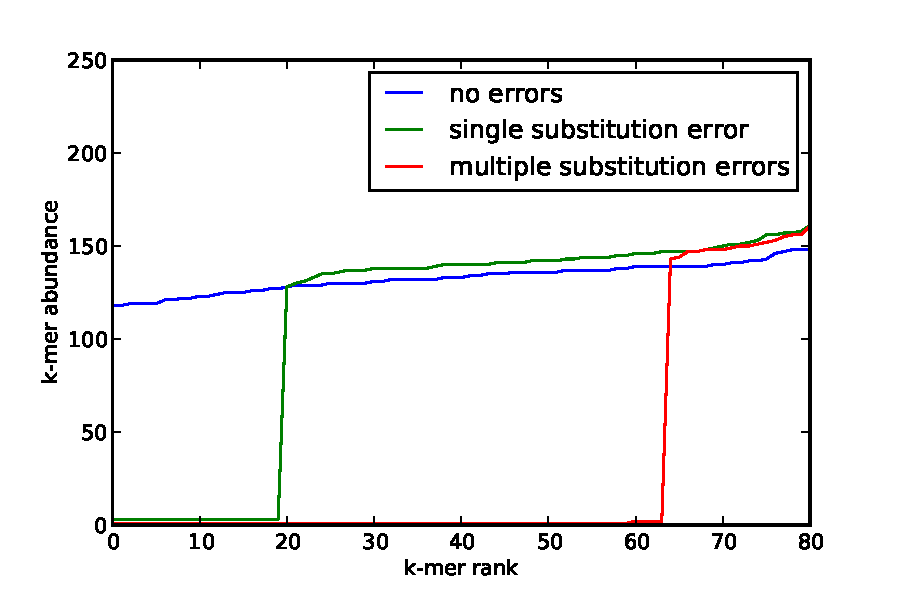
\includegraphics[width=4in]{diginorm-ranks.pdf}}
\caption{
{\bf Representative rank-abundance distributions for 20-mers from 100-base reads with no errors,
a read with a single substitution error, and a read with multiple
substitution errors.}}
\label{fig:rankabund}
\end{figure}

\begin{figure}[!ht]
\begin{center}
\centerline{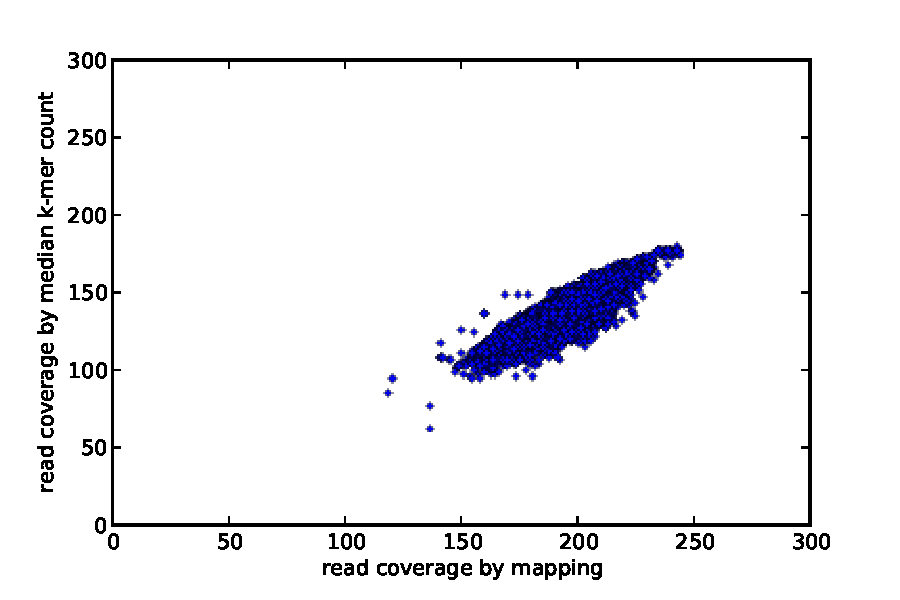
\includegraphics[width=3in]{diginorm-sim-genome.pdf}}
\centerline{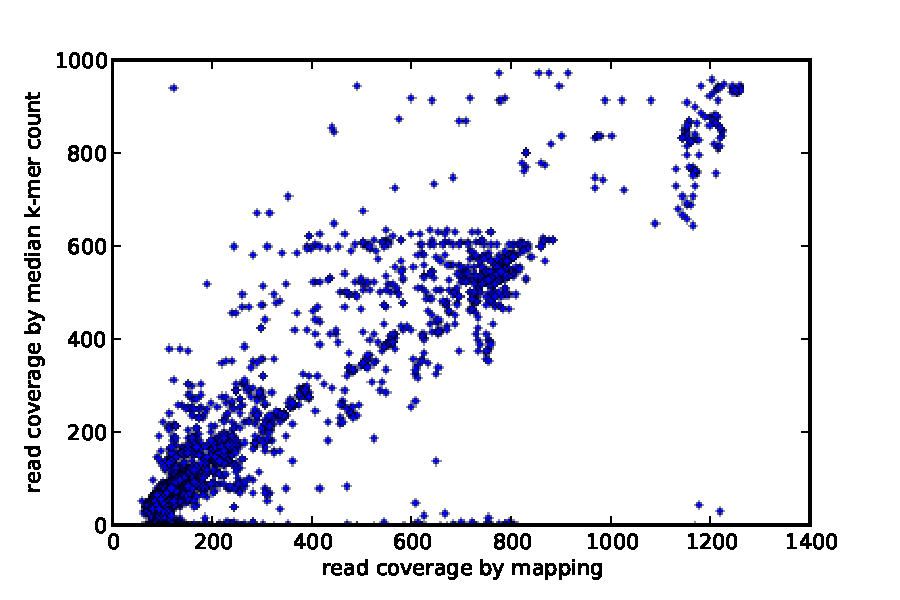
\includegraphics[width=3in]{diginorm-ecoli-genome.pdf}}
\end{center}
\caption{
{\bf Mapping and k-mer coverage measures correlate for simulated genome
data and a real {\em E. coli} data set (5m reads).  Simulated data $r^2 = 0.79$; {\em
E. coli} $r^2 = 0.80$.}
}
\label{fig:random}
\end{figure}

\begin{figure}[!ht]
\begin{center}
\centerline{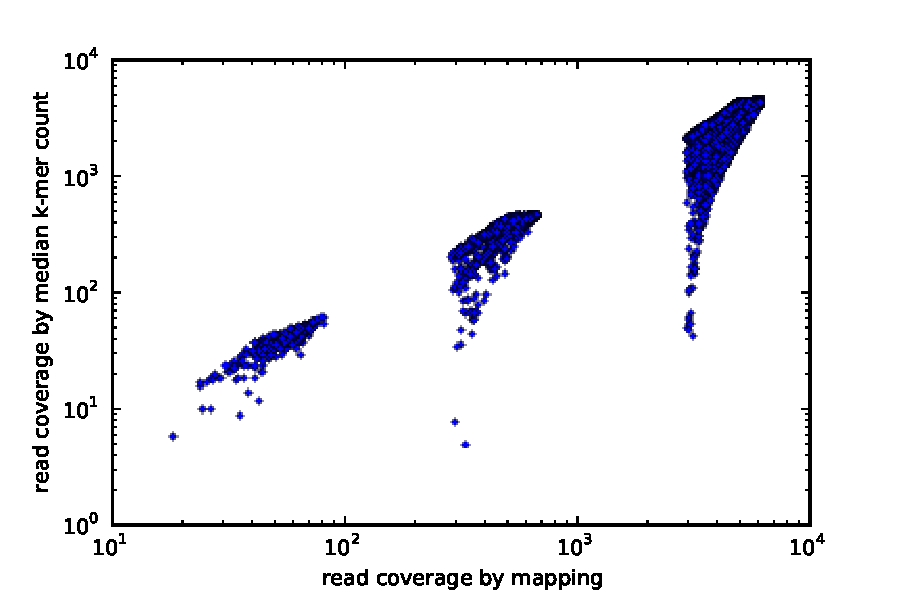
\includegraphics[width=3in]{diginorm-sim-transcr.pdf}}
\centerline{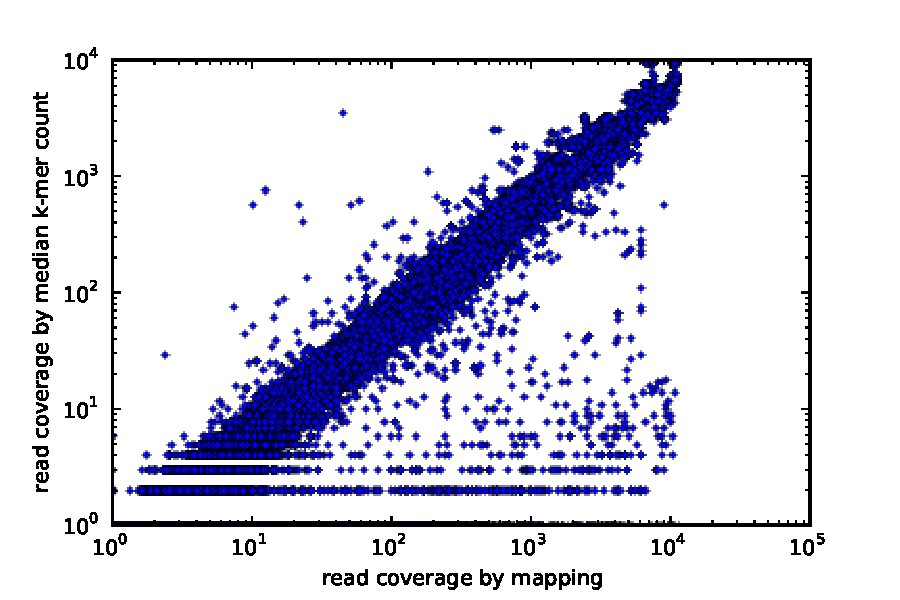
\includegraphics[width=3in]{diginorm-mouse-transcr.pdf}}
\end{center}
\caption{
{\bf Mapping and k-mer coverage measures correlate for simulated transcriptome data as well as real mouse transcriptome data. Simulated data $r^2 = 0.93$;
mouse transcriptome $r^2 = 0.90$.}
}
\label{fig:transcripts}
\end{figure}

\begin{figure}[!ht]
%\centerline{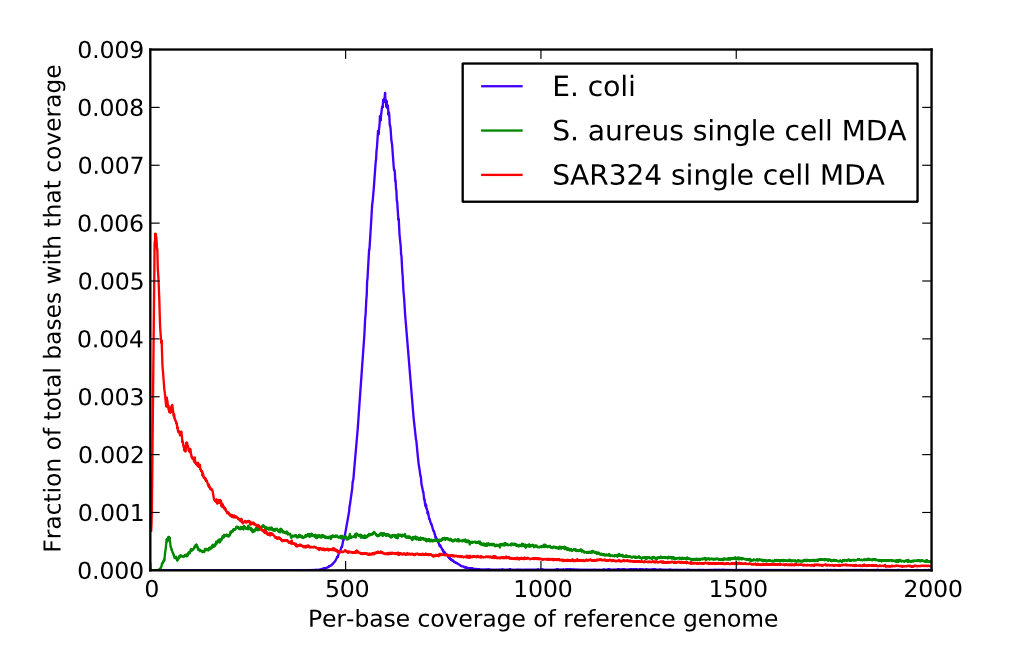
\includegraphics[width=4in]{diginorm-coverage2-raw.pdf}}
%\centerline{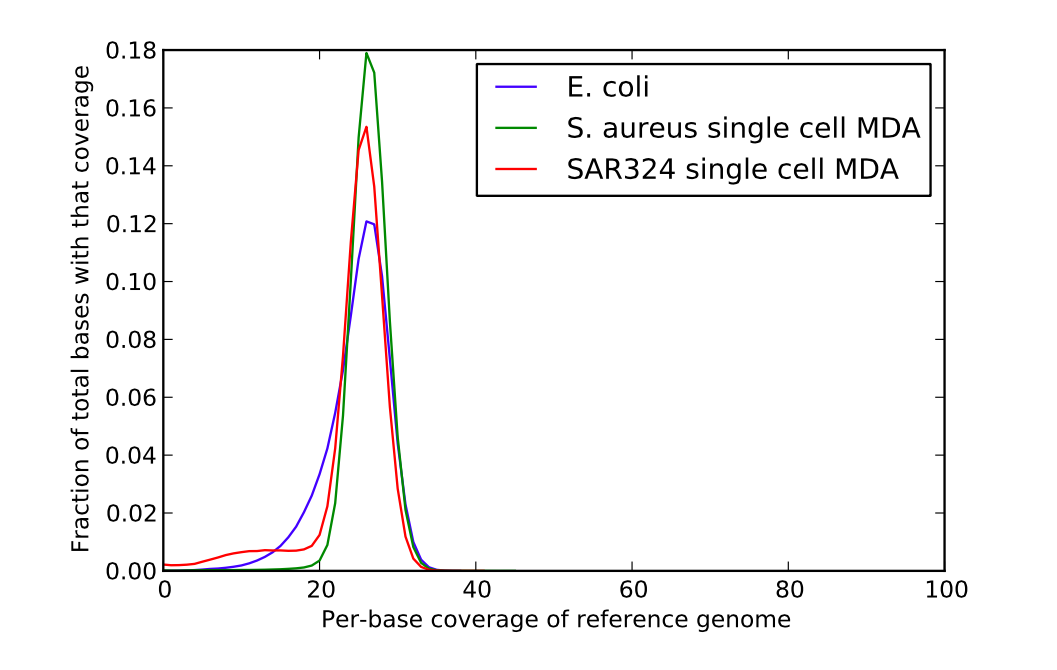
\includegraphics[width=4in]{diginorm-coverage2-dn.pdf}}
\centerline{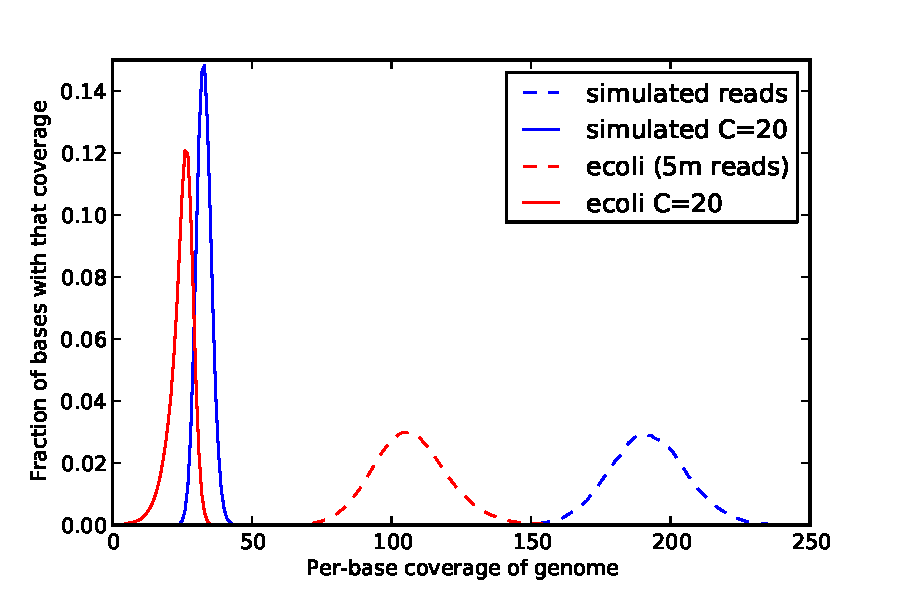
\includegraphics[width=4in]{diginorm-coverage.pdf}}


\caption{
{\bf Coverage distribution of three microbial genome samples, calculated
from mapped reads (a) before and (b) after digital normalization (k=20, C=20).}}
\label{fig:coverage}
\end{figure}

\begin{figure}[!ht]
\centerline{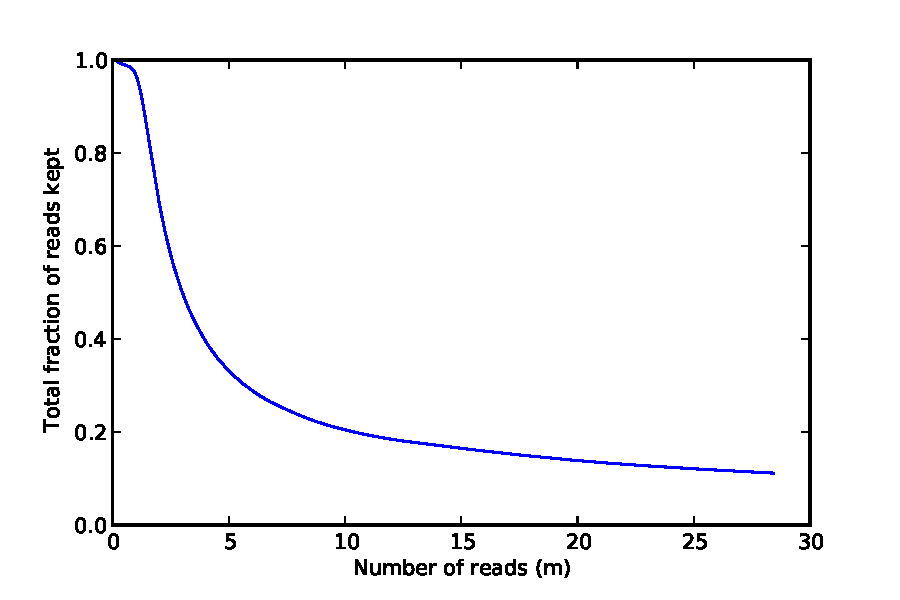
\includegraphics[width=4in]{diginorm-accumulation.pdf}}
\caption{
{\bf Fraction of reads kept when normalizing the {\em E. coli} dataset to C=20 at k=20.}}
\label{fig:accumulate}
\end{figure}

\begin{figure}[!ht]
\centerline{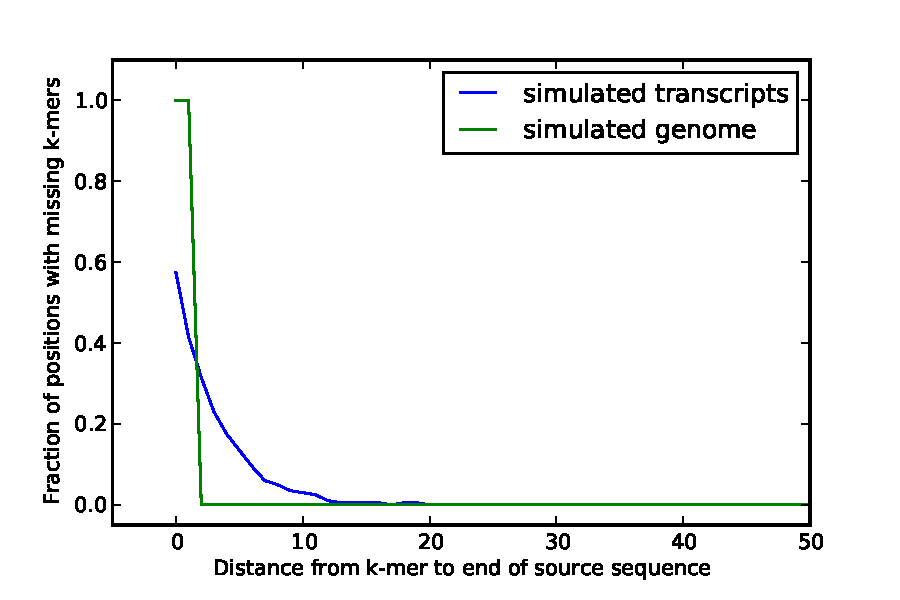
\includegraphics[width=4in]{diginorm-endbias.pdf}}
\caption{
{\bf K-mers at the ends of sequences are lost during digital normalization.}}
\label{fig:endloss}
\end{figure}

%\begin{figure}[!ht]
%\centerline{\includegraphics[width=4in]{schematic.pdf}}
%\caption{}
%\label{fig:schematic}
%\end{figure}

%\begin{figure}[!ht]
%\begin{center}
%%\includegraphics[width=4in]{figure_name.2.eps}
%\end{center}
%\caption{
%{\bf Bold the first sentence.}  Rest of figure 2  caption.  Caption 
%should be left justified, as specified by the options to the caption 
%package.
%}
%\label{Figure_label}
%\end{figure}


\section{Tables}
%\begin{table}[!ht]
%\caption{
%\bf{Table title}}
%\begin{tabular}{|c|c|c|}
%table information
%\end{tabular}
%\begin{flushleft}Table caption
%\end{flushleft}
%\label{tab:label}
% \end{table}

\begin{table}[!ht]
\caption{
\bf{Digital normalization to C=20 removes many erroneous k-mers from sequencing data sets.  Numbers
in parentheses indicate number of true k-mers lost at each step, based on reference.}}
\begin{tabular}{|l|c|c|c|c|c|}
Data set & True 20-mers & 20-mers in reads & 20-mers at C=20 & \% reads kept\\
\hline \\
Simulated genome & 399,981 & 8,162,813 & 3,052,007 (-2) & 19\% \\
Simulated mRNAseq & 48,100 & 2,466,638 (-88) & 1,087,916 (-9) & 4.1\% \\
{\em E. coli} genome & 4,542,150 & 175,627,381 (-152) & 90,844,428 (-5) & 11\% \\
Yeast mRNAseq & 10,631,882 & 224,847,659 (-683) & 10,625,416 (-6,469) & 9.3\% \\
Mouse mRNAseq & 43,830,642 & 709,662,624 (-23,196) & 43,820,319 (-13,400) & 26.4\% \\
\end{tabular}
\begin{flushleft}
\end{flushleft}
\label{tab:normC20}
\end{table}

%@ note that assembly does not exactly match read k-mer content!

%%%%%%%%%%%%%%%%%

\begin{table}[!ht]
\caption{
\bf{Three-pass digital normalization removes most erroneous k-mers.  Numbers
in parentheses indicate number of true k-mers lost at each step, based on known reference.}}
\begin{tabular}{|l|c|c|c|c|}
Data set & True 20-mers & 20-mers in reads & 20-mers remaining & \% reads kept\\
\hline \\
Simulated genome & 399,981 & 8,162,813 & 453,588 (-4) & 5\% \\
Simulated mRNAseq & 48,100 & 2,466,638 (-88) & 182,855 (-351) & 1.2\% \\
{\em E. coli} genome & 4,542,150 & 175,627,381 (-152) & 7,638,175 (-23) & 2.1\% \\
Yeast mRNAseq & 10,631,882 & 224,847,659 (-683) & 10,532,451 (-99,436) & 2.1\% \\
Mouse mRNAseq & 43,830,642 & 709,662,624 (-23,196) & 42,350,127 (-1,488,380) & 7.1\% \\
\end{tabular}
\begin{flushleft}
\end{flushleft}
\label{tab:normC5}
\end{table}

%%%%%%%%%%%%%%%%%%%%%%%

\begin{table}[!ht]
\caption{
\bf{Three-pass digital normalization reduces computational requirements for contig assembly of genomic data.}}
\begin{tabular}{|l|c|c|c|c|}

Data set & N reads pre/post & Assembly time pre/post & Assembly memory pre/post \\
\hline \\
%{\em E. coli} subset & 5m / 0.4m & 235s / 24s (9.8x) & 2.7gb / 0.4gb (6.8x) \\
{\em E. coli} & 31m / 0.6m & 1040s / 63s (16.5x) & 11.2gb / 0.5 gb (22.4x) \\ 
{\em S. aureus} single-cell & 58m / 0.3m & 5352s / 35s (153x) & 54.4gb / 0.4gb (136x) \\
{\em Deltaproteobacteria} single-cell & 67m / 0.4m & 4749s / 26s (182.7x) & 52.7gb / 0.4gb (131.8x) \\

\end{tabular}
\begin{flushleft}
\end{flushleft}
\label{tab:dngenome}
\end{table}



%%%%%%%%%%%%%%%%%%

\begin{table}[!ht]
\caption{
\bf{Single-pass digital normalization to C=20 reduces computational
requirements for transcriptome assembly.}}

%add yeast

\begin{tabular}{|l|c|c|c|c|}

Data set & N reads pre/post & Assembly time pre/post & Assembly memory pre/post \\
 \hline \\
Yeast (Oases) & 100m / 9.3m & 181 min / 12 min (15.1x) & 45.2gb / 8.9gb (5.1x) \\
Yeast (Trinity) & 100m / 9.3m & 887 min / 145 min (6.1x) & 31.8gb / 10.4gb (3.1x) \\
Mouse (Oases) & 100m / 26.4m & 761 min/ 73 min (10.4x) & 116.0gb / 34.6gb (3.4x) \\
Mouse (Trinity) & 100m / 26.4m & 2297 min / 634 min (3.6x) & 42.1gb / 36.4gb (1.2x) \\
\end{tabular}

\begin{flushleft}
\end{flushleft}
\label{tab:dntrans}
\end{table}

%%%%%%%%%%%%%%%%%%%%%%%%%%%

\begin{table}[!ht]
\caption{
\bf{Digital normalization has assembler-specific effects on transcriptome
assembly.}}

%add yeast

\begin{tabular}{|l|c|c|c|c|}

Data set & Contigs $>$ 300 & Total bp $>$ 300 & Contigs $>$ 1000 & Total bp $>$ 1000 \\
\hline \\
Yeast (Oases) & 12,654 / 9,547 & 33.2mb / 27.7mb & 9,156 / 7,345 & 31.2mb / 26.4mb \\
Yeast (Trinity) & 10,344 / 12,092 & 16.2mb / 16.5mb & 5,765 / 6,053 & 13.6 mb / 13.1mb \\
Mouse (Oases) & 57,066 / 49,356 & 98.1mb / 84.9mb & 31,858 / 27,318 & 83.7mb / 72.4mb \\
Mouse (Trinity) & 50,801 / 61,242 & 79.6 mb / 78.8mb & 23,760 / 24,994 & 65.7mb / 59.4mb \\

\end{tabular}

\begin{flushleft}
\end{flushleft}
\label{tab:dntrans0}
\end{table}

\chapter{concept and simulation}



\section{Introduction}

In almost all  metagenomics projects, diversity analysis plays an important
role to supply information about the richness of species, the species abundance
distribution in a sample or the similarity and difference between different 
samples, all of which are crucial to draw insightful and reliable conclusion. 
Traditionally especially for amplicon metagenomics data set, OTUs(Operational 
Taxonomic Units) based on 16S rRNA genes are used as the basic units for 
diversity analysis. OTUs can be good replacement of the concept of "species" in 
metagenomics. Basically contigs are assembled from reads and are "binned" into
OTUs using composition-based or similarity-based approaches. Then the diversity
can be estimated by using the abundance information of the OTUs.

% from proposal, need to be rewritten to be more precise.
Recently there are many more projects generating whole genome shotgun metagenomics data sets. However they are 
mainly used for assembly and annotation purpose. Less attention was paid to diversity measurement
using these whole genome metagenomics data sets. One possible reason is that the whole genome metagenomics
data sets are often with low depth given the high diversity of metagenomics samples compared to 16S rRNA
ampicon metagenomics data set. Assembly and annotation are always challenging with the low depth and lack of 
reference sequences. It is also true for diversity measurement. On the other hand, although with low depth, some whole genome metagenomics 
data sets are with large size because of the high diversity. For instance, there may be 4 petabase
pairs of DNA in a gram of soil{Zarraonaindia:2013aa}. Many of those methods for sequence binning or diversity 
estimation do not scale well and will not work for large metagenomics data sets. For instance,
many composition-based binning approach involves k-mer/signature frequency distribution calculation, which is 
rather computationally expensive. Even basic sequence alignment will be impossible for large metagenomics data set.
Many of those statistical software packages to estimate diversity using various estimators are not prepared 
for the large scale of whole genome metagenomics data. 

With the development of next generation sequencing technology, the cost of sequencing is dropping rapidly. 
Whole genome metagenomics sequencing is more popular and large amount of metagenomics data is 
being generated with increasing speed, which can not be even met by the increase of computational capacity.
Novel methods that can scale well are extremely needed to deal with the increasingly large metagenomics data
set. 


%diversity analysis, is the central topic of in microbial ecology.
%
%
%1. traditionally, OTU 
%
%2. assembly, annotation, 
%megan, 
%
%binning
%
%3. co abundance methods.
%
%4. alpha , genome size estimation.
%
%5. igs, better , advantage
%
%alpha, beta 
%
%
%
%assembly, contig binning
%
%no assembly, no reference sequence
%
%
%kmer couting, 
%
%paper:
%
%alpha, co abundance, 
%beta, co abundance across samples
%
%
%
%
%khmer counting,
%
%streaming, diginorm, 
%


Here we propose a novel concept - IGS (informative genomic 
segment) and use IGS as a replacement of OTUs to be the cornerstone for 
diversity analysis of whole shotgun metagenomics data sets. IGSs represent the 
unique information in a metagenomics data set and the abundance of IGSs in 
different samples can be retrieved by the reads coverage through an efficient 
k-mer counting method. This samples-by-IGS abundance data matrix is a promising
replacement of samples-by-OTU data matrix used in 16S rRNA based analysis and 
all existing statistical methods can be borrowed to work on the samples-by-IGS 
data matrix to investigate the diversity. We applied the IGS-based method to 
several simulated data sets and a real data set - Global Ocean Sampling 
Expedition (GOS) to do beta-diversity analysis and the samples were clustered 
more accurately than existing alignment-based method. We also tried this novel 
method to Great Prairie Soil Metagenome Grand Challenge data sets. Furthermore 
we will show some preliminary results using the IGS-based method for 
alpha-diversity analysis. Since this method is totally binning-free, 
assembly-free, annotation-free, reference-free, it is specifically promising 
to deal with the highly diverse samples, while we are facing large amount of 
“dark matters” in it, like soil.




\section{The concept of IGS(informational genomic segment)}

In classic ecology dealing with macroorganisms, diversity measurement is based 
on the concept of species. For 16S rRNA amplicon metagenomics data set, it is 
based on the concept of OTUs. While the concept of OTUs can be used to analyze
large shotgun metagenomics data set, normally assembly, binning and annotation
are required before doing diversity analysis. However these are difficult
tasks, lacking of necessary reference genome or being computationally
expensive. So we are interested in finding an approach to bypass the difficult
tasks like assembly, binning, annotation and use raw reads to make diversity
analysis to large metagenomic data possibile. In the beginning we proposed that
 the concept of k-mers(a DNA segment with the leng of k) can be used to measure
 diversity. K-mers can be considered as the atom of information in DNA 
sequences. One of the composition-based approaches to binning is to use the 
k-mer as the signatures. Suppose the sizes of microbial genomes are similar and
 the difference between genomic content of microbial genomes is similar, the 
number of distinct k-mers in the sequence data set correlates to the number of 
species in a sample. However, because of sequencing error, which is unavoidable
 due to the limit of sequencing technology, this k-mer based analysis doe not 
work well. One sequencing error on a read will generate at most k erroneous 
k-mers. In metagenomics data set, especially with high coverage, most of the 
distinct observed k-mers are from sequencing errors.
%add citation about k-mer based diversity analysis ,entropy...
% add some results /figures

Next we looked at the upper level - reads. A novel method termed as digital 
normalization was developed to remove abundant reads before assembly. However 
it also supplies a novel way to distil information from reads by reducing the
 bad effect of sequencing errors so that we can use those informative reads to 
measure the microbial diversity. We term those informative reads as 
IGS(informative genomic segment), which can be considered as a segment of DNA 
on a microbial genome. Those IGSs should be different enough to represent the 
abstract information a genome contains. Suppose microbial genomes contain 
similar number of those IGSs, as they contain similar number of distinct 
k-mers, the number of IGSs will correlates with the species richness in a 
sample, and the abundance distribution of IGSs will be related to species 
evenness in a sample. Furthermore, we can get the abundance of the IGSs across
different samples. Many classic diversity estimation methods based on OTUs 
 described in sections above can be applied to estimate the diversity of IGSs 
and the diversity of actual species subsequently.

The concept of IGS can be the foundation of a novel statistical framwork to
evaluate microbial diversity using whole genome shotgun metagenomic data, 
especially while facing large amount of "dark matters", unknown species. It is
almost impossible to do annotation to those "dark matters", since we do not
have much information about them. 
% need expanding
For alpha diversity, we can generate a list of IGSs and the respective 
abundance in a sample. Then existing estimators like Chao's can be used to 
estimate the total number of IGSs in the sample. Rarefaction curve based on 
number of IGSs can also be generated. 

% need expand the discussion from IGS in one sample to IGS in different samples.
For beta diversity, we can generate a samples-by-IGS data matrix from the
abundance of IGSs across samples, as a replacement of samples-by-OTU data 
matrix in OTU-based analysis and samples-by-species data matrix in traditional 
ecology. From that samples-by-IGS data matrix, we can use existing methods to 
calculate similarity/disimilarity/distance between samples and do further 
analysis like clustering and ordination. 

% further application
% With the samples-by-IGS data matrix, it is also possible to calculate similarity between IGSs and do ordination, which is a potential approach to classify IGS( reads).

%Using simulated and real genomic data sets, with the help of khmer to get median k- mer abundance, we find that median k-mer abundance correlates well with mapping-based coverage.

%Side note: We can also see that the coverage by median k-mer count is generally lower than the read coverage by mapping. So estimation of sequencing coverage by median k-mer count is underestimated. This can cause some problems in later analysis, which will be discussed later.


\subsection{IGS(informative genomic segment) can represent the novel 
information of a genome}

Median k-mer abundance can represent sequencing depth of a read(cite diginorm).
 For a sequencing reads data set with multiple species, the sequencing depth of
 a read is related to the abundance of species where the read originates. 

% figure 1a should be marked 
The Figure \ref{fig:reads_to_IGS}a  shows the abundance distribution of reads 
from 4 simulated sequencing data sets with different sequencing depth - 3 
sequencing data sets generated with different sequencing coverage(1x, 10x, 40x)
 from 3 simulated random genomes respectively and 1 combined data set with all 
the previously mentioned data sets. No error is introduced in these simulated 
data sets. Obviously the reads from the three data sets can be separated by 
estimated sequencing depth. The combined data set can be considered as a 
sequencing data set with three species with different abundance.

Each point on the curve shows that there are Y reads with a sequencing depth of
 X. In other word, for each of those Y reads, there are X-1 other reads that 
cover the same DNA segment in a genome that single read originates. So we can 
estimate that there are Y/X distinct DNA segments with reads coverage as X. 
We term these distinct DNA segments in species genome as 
IGS(informative genomic segment). We can transform the figure in upper 
position to show the number of IGSs and their respective reads coverage, as 
shown in figure in lower position. We sum up the numbers of IGSs with 
different reads coverage for each data set and get the result as shown in 
below. The sum numbers of IGSs here essentially are the areas below each curve 
in the figure.

Even though the datasets have different sequencing depth like 10X and 40X, 
they have similar numbers of IGSs. Dataset with 1X sequencing depth has fewer 
IGSs because the depth is not enough to cover all the content of the 
genome(63.2\%). The IGSs can be seen as the
genomic segment on a genome with the length of reads.(Figure \ref{fig:IGS}  
Assume the species 
genome is totally random, which is the case in the simulated data set, the 
number of IGSs(N) in a species genome is related to the size of genome(G), 
read length(L) and k size(k), which can be denoted as

\[N =\frac{G}{L}  \]
which is the number of reads that can have a 1X coverage of the genome.
For the simulated genome with size of 1M bps, read length as 80bps, expected 
number of IGSs is 

1000000/(80 - 22 + 1) = 16949, 

which is pretty close to observed value. See Table \ref{table:IGSs}
((((((( This needs rewrite, the table will be replaced)))))))))))

\begin{figure}[!ht]
\centerline{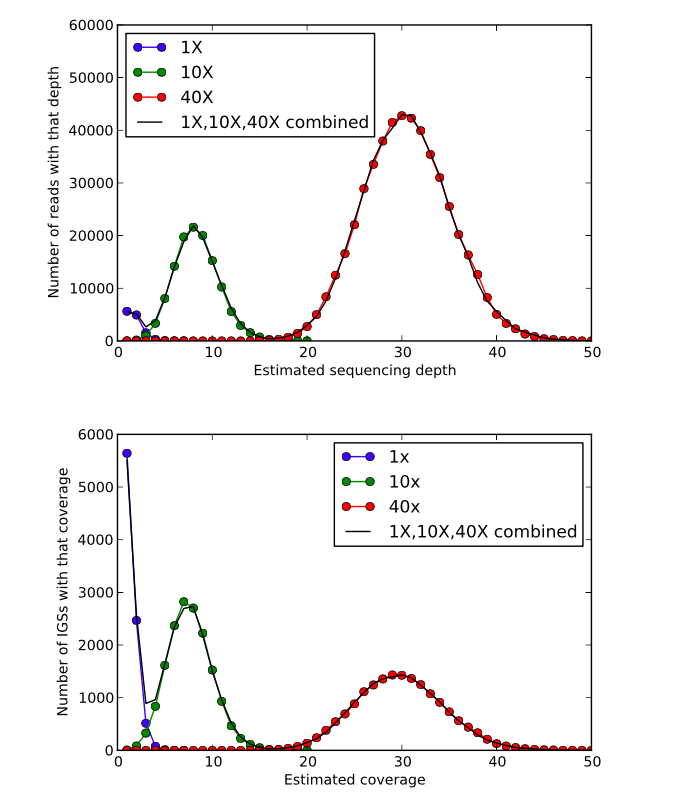
\includegraphics[width=4in]{./figures/from_reads_to_IGS.png}}
%\caption{\bf cluster of GOS samples using IGS method}
\caption{\bf from reads to IGS}
\label{fig:reads_to_IGS}
\end{figure}

\begin{table}[!ht]
\caption{
\bf{Total number of IGSs in different simulated reads data sets.}
}
\begin{tabular}{ |c | c |c| c|c| }
Data set & total number of IGSs \\
\hline \\
1X depth                   & 8714  \\
10X depth                  & 16321  \\
40X depth                  & 16794 \\
1X,10X,40X combined        & 41742 \\
\end{tabular}
\begin{flushleft}
\end{flushleft}
\label{table:IGSs}
\end{table}


\begin{figure}[!ht]
\centerline{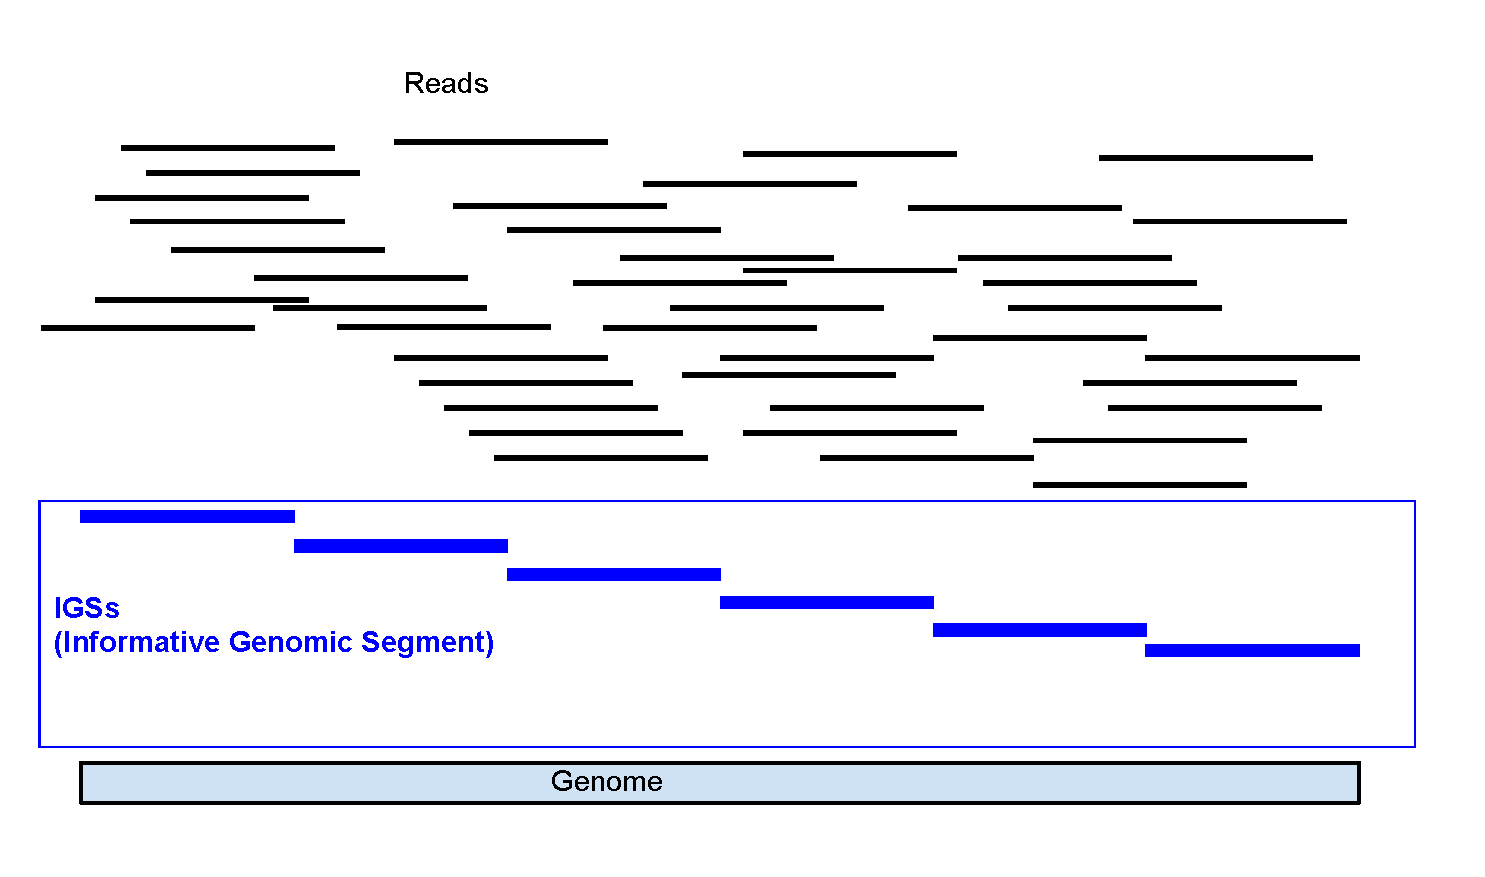
\includegraphics[width=4in]{./figures/IGSs_figure.pdf}}
\caption{\bf the concept of IGS}
\label{fig:IGS}
\end{figure}





\subsection{IGS can be used to do alpha diversity analysis}

Basically the abundance distribution of IGSs with different coverage in a sample data set is acquired using the method shown above, like:
\\
3 23\\
4 24\\
5 25\\
6 25\\
...\\
\\
Here 23 IGSs with coverage as 3, this number is calculated from dividing the total number of reads with coverage as 3, which is 69, by the coverage 3: 69/3. Similarly there are 96/4 = 24 IGSs with coverage as 4.

If we draw an analogy between IGSs and OTUs, this is like there are 23 different OTUs with 3 reads mapped to, and 24 different OTUs with 4 reads mapped to. 

Then list all the different IGSs and the corresponding count,and we can get a long list with each IGS and the corresponding coverage.The coverage of an IGS can be considered as the abundance of such IGS in a sample. The list looks like:
\\
IGS\_ID abundance\\
1     3\\
2     3\\
3     3\\
 ...\\
23    3\\
24    4\\
25    4\\
...\\
47    4\\
48    5\\
 ...\\
 ...\\
  
This list is the counterpart of an OTU table in OTU based diversity analysis.

With such table at hand, numerous existing statistical methods and software packages can be used to investigate the alpha diversity.  



\subsection{IGS can be used to do beta diversity analysis}

As in alpha diversity analysis, OTU table is also a cornerstone for beta diversity analysis. As long as we get a reliable OTU table, there are existing pipelines to do the beta diversity analysis. 

A typical OTU table across different samples is like this, which is also called samples-by-OTU data matrix.
\\
OTU\_ID Sample1\_ID Sample2\_ID Sample3\_ID\\
OTU1   3          4          2\\
OTU2   2          5          0\\
OTU3   3          1          4\\
\\
    
Like a OTU table, we hope to have the IGS table for the IGSs:
\\
    IGS\_ID SampleA SampleB SampleC SampleD\\
    IGS1   5       1       2       1\\
    IGS2   5       1       2       1\\
\\
    
    So now the problem is how we can generate a sample-by-IGS data matrix as the counterpart of samples-by-OTU data matrix so many of  the existing tools/methods used for OTU-based diversity can be borrowed for this kind of IGS-based analysis, just as what is shown above for alpha diversity analysis.

Firstly, as how we get the coverage of a read from a sample dataset in this sample dataset, we can get the coverage of a read from a sample A dataset in another sample B dataset. We can still use the median k-mer count to represent the coverage. The basic idea is the same. 

Because a read must derive from a segment in the genome of some species in a sample, if a read R from sample A with a coverage C\_A in sample A has a coverage as C\_B in sample B, that means that segment of genome in sample A from which read R derive also exists in sample B. That genomic segment has a coverage as C\_A in sample A and has a coverage as C\_B in sample B. Roughly there should be about C\_A reads (read R should be one of them) in sampleA covering that genomic segment and C\_B reads in sampleB covering that genomic segment. Meanwhile, the C\_A reads in sampleA should all have a coverage as C\_B in sampleB, just like read R as one of them. Similarly, the C\_B reads in sampleB should all have a coverage as C\_A in sampleA.

Ok, now let's make an example. 

Suppose there are 6 reads in sample A, all have a coverage as 3 in sampleA, and have a coverage as 2 in sampleB.

According to the discussion about IGS in previous section, the 6 reads cover 2 IGSs with a coverage as 3 for each IGSs. There should be 4 reads in sampleB covering the exact same 2 IGSs, with a coverage as 2 in sampleB.

So now we have 2 distinct IGSs with redundancy as 3 and 2 in the two samples respectively. 

**Note:** small number is used in the analysis above as example, but it should be emphasized that the analysis is based on large number statistically.


Let's expand this example from 2 samples to 4 samples(A,B,C,D), as shown in figure above.

Let's say we find 10 reads in sampleA, with coverage as 5-1-2-1 in samples A-B-C-D respectively. (We call "5-1-2-1" "coverage  spectrum" across samples.) So there should be **about** 2 reads in sampleB, 4 reads in sampleC, 2 reads in sampleD, all of which have a "coverage spectrum" as "5-1-2-1". Basically these 18 reads altogether cover 2 distinct IGSs, which apparently exist in all the 4 samples. The 2 distinct IGSs has a redundancy as 5,1,2,1 in the 4 samples respectively.

If we draw an analogy between IGSs and OTUs, this is like there are 2 OTUs, both with 5,1,2,1 reads mapped to in sample A,B,C,D respectively.

Like a OTU table, here we can have the IGS table for the two IGSs:
\\
    IGS\_ID SampleA SampleB SampleC SampleD\\
    IGS1   5       1       2       1\\
    IGS2   5       1       2       1\\
\\
    
 % should all include alpha and beta diversity results
\section{Evaluating IGS method using simulated data sets}
\subsection{An experiment using a simple simulated data sets}

For this experiment, firstly we create 6 synthetic samples (Sample 1-6) based on 9 synthetic 10K genomes (genome A-I), with different composition of species and diversity. 

The  species composition for each synthetic sample is as below:

sample1: AAAB

sample2: AABC

sample3: ABCD

sample4: ABCE

sample5: AFGH

sample6: IFGH

For sample1, there are two species - A and B, with abundance distribution as 3:1.

The sequencing depth of all the synthetic data sets is 10X. So the species abundance in each sample is as below:

sample1: genomeA - 30, genomeB - 10

sample2: genomeA - 20, genomeB - 10, genomeC - 10

sample3: genomeA - 10, genomeB - 10, genomeC - 10, genomeD - 10

sample4: genomeA - 10, genomeB - 10, genomeC - 10, genomeE - 10

sample5: genomeA - 10, genomeF - 10, genomeG - 10, genomeH - 10

sample6: genomeI - 10, genomeF - 10, genomeG - 10, genomeH - 10


An a simple experiment, there is no sequencing errors introduced in the synthetic reads data sets.

Figure \ref{fig:simple_pcoa} and Figure \ref{fig:simple_cluster} show that IGS method can yield the information 
about the difference of samples correctly. Sample 5 and sample 6 and very close to each other on the figure, which 
is true if we check the species composition of the two samples shown above.

Figure \ref{fig:simple_alpha} shows the  method can yield the richness information correctly. From the figure, samples with 
4 different species have the richness almost twice as large as the sample with 2 different species. 

From these results, we show the IGS method can work well to a simplest scenario, with high sequencing depth (10X) and no sequencing error. Next we will check the influence to the analysis accuracy of variable sequencing depth and sequencing error and introduce new ways to preprocess the data to decrease the influence of sequencing error. 


\begin{figure}[!ht]
 \centerline{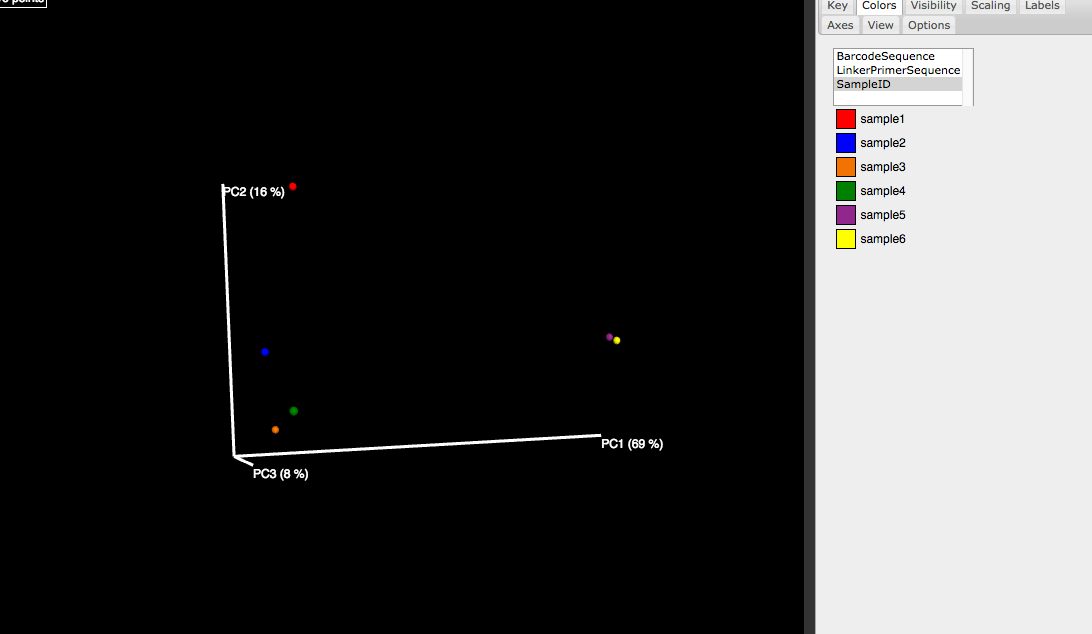
\includegraphics[width=4in]{./figures/simple_PCA_3d.png}}
\caption{\bf Ordination of the 6 synthetic samples using IGS method}
\label{fig:simple_pcoa}
\end{figure}


\begin{figure}[!ht]
 \centerline{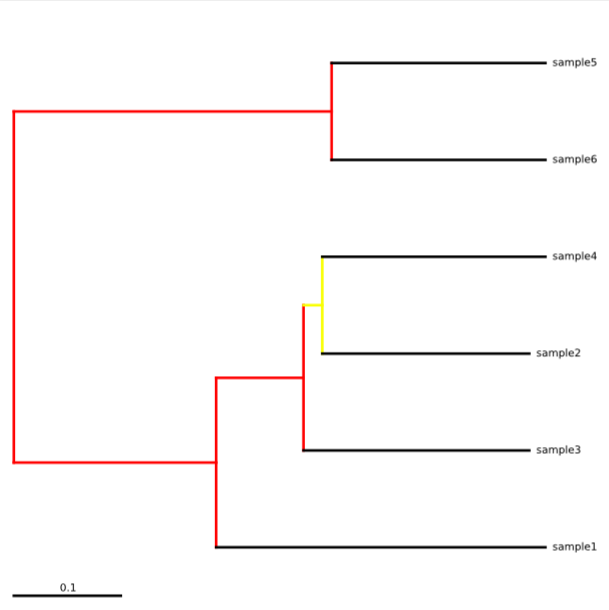
\includegraphics[width=4in]{./figures/simple_tree.png}}
\caption{\bf Clustering of the 6 synthetic samples using IGS method}
\label{fig:simple_cluster}
\end{figure}


\begin{figure}[!ht]
 \centerline{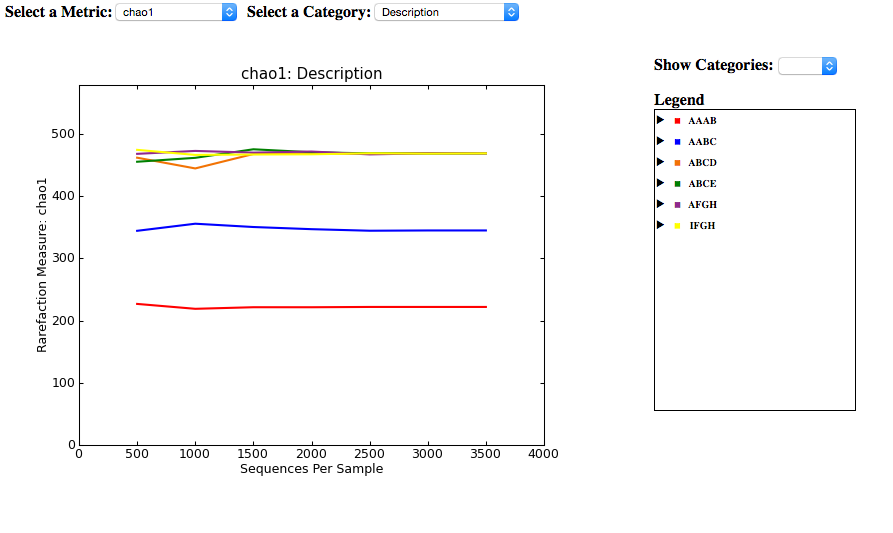
\includegraphics[width=4in]{./figures/simple_chao_alpha.png}}
\caption{\bf Richness estimation of the 6 synthetic samples using IGS method}
\label{fig:simple_alpha}
\end{figure}


\subsection{Improving the accuracy of this method in real world analysis}


Previously we have shown the IGS method generally works to a simple simulated
 data sets, with high sequencing depth and no sequencing error. In real world,
in many situations we have to deal with the metagenomic data sets with 
relatively low sequencing depth, like soil or sea water samples. 
Also it is a fact that all sequencing technology will generate some errors. As 
discussed in the background 
section, one of the reasons we develop the IGS method is that based on the 
abundance counting of reads rather than k-mers, it is expected that the IGS 
method is less prone to sequencing error. However the effect of those factors 
jeopardizing the accuracy is still observable. 

In this section, we will analyze the effect of these factors to the accuracy of
 the IGS method and investigate the ways to reduce the effect to increase the 
accuracy of analysis.


As in last section, six synthetic samples were generated with the same species 
composition . For each sample, sequencing reads data sets with different
sequencing depth(0.1X, 1X, and 10X) and different sequencing error rate (0.5\%,
 1.0\%, 1.5\%, and 0\% - no error at all) are simulated.

To show the effect of sequencing error to accuracy of the 
analysis, we compared the richness estimation using reads with different 
sequencing error rate, as shown in Figure \ref{fig:IGS_richness_no_adjustment}. 
For data set without error (error rate = 0), the esimated size of metagenome
matches real size perfectly. With increasing error rate, the size of metagenome
is over estimated more and more seriously. This is due to several factors,which
will be discussed below. 
\begin{figure}[!ht]
 \centerline{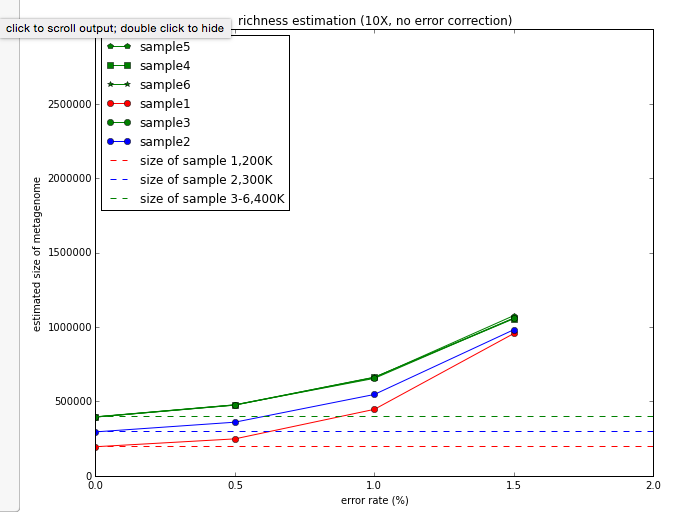
\includegraphics[width=4in]{./figures/IGS_richness_no_adjustment.png}}
\caption{\bf Richness estimation using IGS method without adjustment}
\label{fig:IGS_richness_no_adjustment}
\end{figure}

\subsubsection{the effect of sequencing error to the accuracy of analysis}
The first factor to take into account is sequencing error. One sequencing error
will generate k erroneous k-mers. This is the reason why it is difficult to use
k-mer counting only to do diversity analysis, as a large proportion of k-mers
in a reads data set are erroneous, especially for low coverage reads data. As
discussed in the section about digital normalization, using median k-mer count
to retrieve the coverage of a read is less prone to sequencing error, because
sequencing error will decrease the count of some reads to 1 incorrectly, but
this does not always affect the median k-mer count. 

Take the experiment we did
previously as an example, for read length as 100bp and k as 19, one sequencing
error will affect the count of 19 k-mers at the most, two sequencing errors
will affect the count of at most 38 k-mers. The count of these k-mers will be
retrieved as 1 incorrectly, suppose it is highly impossible that an erroneous
k-mer is the same as another real k-mer in the data set accidently, as long as
the k is large enough compared to the size of data set. So out of the 82 k-mers
in the 100bp read, at most 38 k-mers will have count as 1 incorrectly, but this
will not affect the median k-mer count, which is the count of the 41th k-mer if
ranked by count. However, if there are three or more errors in the read, the 
situation is more complicated. For 3 errors in a read, 3 to 57 k-mers
will be affected by the errors to have an incorrect count as 1. The 
distribution of the probability about the number of affected k-mers can be
acquired by a model similar to Lander-Waterman model used in genome sequencing
 theory. Here we got the distribution using simulation, as shown in Figure
\ref{fig:IGS_affected_k_kmers}. From this probability distribution, we can get
the probability that 3 errors will affect more than 40 k-mers is 0.43. In this
case, 3 errors will affect the median k-mer count of a read. We can also get 
such probability for 4 errors or more. Combining to the probability that a
certain number of errors occur in a read with a specific sequencing error rate,
which is easy to derive from binomial distribution, we can get the probability
that the coverage of a read is incorrectly assessed as 1. Still for the example
here, this probability is the probability that 3 erorrs occur in a read
multiplied by the probability that 3 errors will affect median k-mer count,
plus the probability that 4 erorrs occur in a read multiplied by the 
probability that 4 errors will affect median k-mer count,and so on.

Generally, let $P\_error(n,e,L)$ is the probability that $n$ errors occur in a 
read with length as $L$, with error rate as $e$ and $P\_effect(n,k,L)$ is the 
probability that $n$ 
errors in a read with length of $L$ affect median k-mer count. The probability 
that the coverage of a read is incorrectly assessed as 1 is 
\[\sum_{n=3}^{\infty} P\_error(n,e,L) \times P\_effect(n,k,L)  \],
and by binomial distribution,

\[P\_error(n,e,L) = f(n;L,e) = Pr(X=n) = {L \choose n}e^n(1-e)^{L-n} \] 

Practically, when $n>5$ and $e<0.015$, $P\_error(n,e,L)$ is very small, we only consider
number of errors in a read as 3, 4 and 5.

\begin{figure}[!ht]
 \centerline{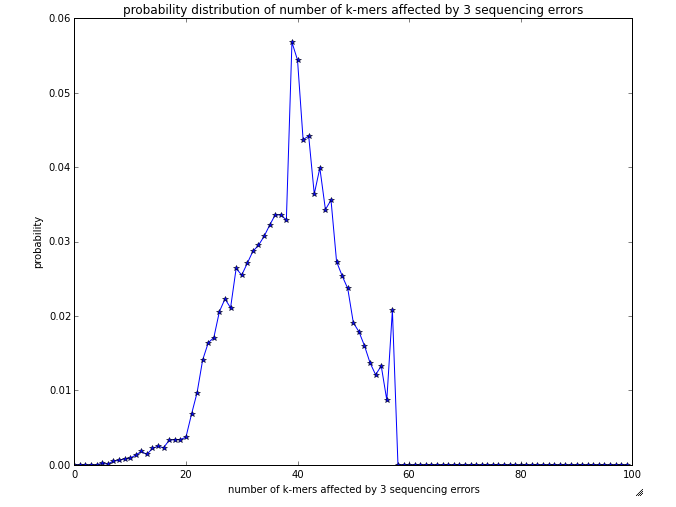
\includegraphics[width=4in]{./figures/IGS_affected_k_kmers.png}}
\caption{\bf Richness estimation using IGS method without adjustment }
\label{fig:IGS_affected_k_kmers}
\end{figure}

From the discussion above, the sequencing errors reduce the coverage of some
reads incorrectly to 1 and the probability this occurs to a read can be
estimated. So to reduce the effect of sequencing error on this aspect, we can
calculate the expected number of reads that are affected and remove those reads
from the set of reads with coverage as 1 before generating list of IGS from the
reads abundance distribution.

Also, we want to make sure 2 errors in a read will not affect median k-mer 
count, since it is more common to have 2 errors in a read practically. 
In this case, 
\[2 \times k < \lfloor \frac{L-k+1}{2}\rfloor \],
we can get $k<L/5$,basically. For $L$ as 100, $k$ will be 19, which is what we 
choose in the testing. However, the $k$ should not be too small, or the k-mers 
can not handle the information of a large data set.

Taking the sequencing error into account, we used the methods introduced above
to adjust the estimation of metagenome size of the 6 synthetic samples. The
estimation after adjustment is closer to real number, as shown in Figure
\ref{fig:IGS_richness_error_adjustment}..


\begin{figure}[!ht]
 \centerline{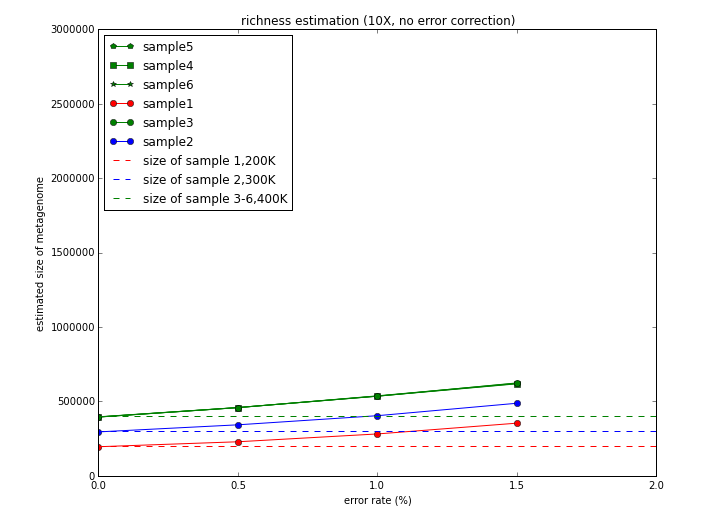
\includegraphics[width=4in]{./figures/IGS_richness_error_adjustment.png}}
\caption{\bf Richness estimation using IGS method adjusted by sequencing error rate}
\label{fig:IGS_richness_error_adjustment}
\end{figure}

\subsubsection{the effect of collision in bloom filter to analysis accuracy}
As discussed in the chapter about k-mer counting, the collision in bloom filter
which we use for efficient k-mer counting will result in counting error. If the
false positive rate for a specific bloom filter we use for k-mer counting is
0.1, 10\% of the k-mers will have incorrect counts. When we use median k-mer
count to get read coverage, such incorrect count has the effect on two aspects.
On one hand, some k-mers in a read will have incorrect higher count. But if the
 false
positive rate is low, this will not affect median k-mer count. This shows the
method of using median k-mer count to get read coverage is not only less prone
to sequencing error, but also less prone to the inaccuracy characteristics of
underlying data structure. One the other hand, this inaccurate count also
affects the counts of those erroneous k-mers generated by sequencing error. For
example, 3 errors in a read affect the count of 43 k-mers, the counts for these
43 k-mers are supposed to be 1. But because of the collision in bloom filter
and the resulting incorrect k-mer counting, if the false positive rate is 0.1,
about 4 out of the 43 k-mers will have inflated count, mostly as 2. So the
combined effect of sequencing error and collision in bloom filter is that some
reads will have incorrect coverage as 1 and some reads will have incorrect as
2. We can get the percentage of total reads that will have such incorrect
coverage, using statistical model similar to that discussed in last section.
Using same example, 3 errors occur in a read, if the 3 errors affect 41-45
k-mers(with a chance of 0.20), the median k-mer count will be 2, due to the 
collison in bloom filter, while if he 3 errors affect more than 45 k-mers(with 
a chance of 0.24), the median k-mer count will be 1, purely due to sequencing 
errors. 

We did the same experiment but also adjusted the estimation according to the 
false positive rate of bloom filter and got better estimation, as shown in
Figure \ref{fig:IGS_richness_adjustment}.

With adjustment to estimation taking sequencing error and collision in bloom
filter into account, as shown in Figure \ref{fig:IGS_richness_adjustment}, the 
estimated genome size is closer to real number. With error rate as 1\%,
false positiver rate as 0.1, with 10X coverage data, the estimated genome size
is about 20-25\% more than real number. However the estimation is still 
increasing with higher
error rate. This means there are still other factors influencing this
accuracy of the estimation but we failed to take into account.

The other problem is that the result of low coverage data(0.1x) is worse than
before adjustment. This may be due to the smaller number of reads with 
abundance of 2 after adjustment. It may also be due to small size of simulated 
data (with only hundreds of reads).


\begin{figure}[!ht]
 \centerline{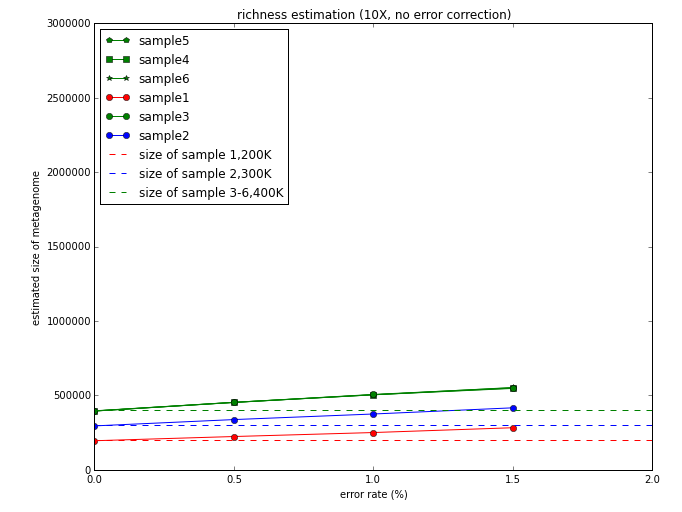
\includegraphics[width=4in]{./figures/IGS_richness_adjustment.png}}
\caption{\bf Richness estimation using IGS method adjusted by sequencing error
rate and false positive rate of bloom filter}
\label{fig:IGS_richness_adjustment}
\end{figure}

\subsubsection{comparison of dissimilarity matrix from beta diversity analysis}

To evaluate the effectiveness of beta diversity analysis using IGS based method, we compare the dissimilarity matrix generated by IGS based method with that generated from another metagenomics comparison tool - Commet(Compareads), and the true matrix,since we know exactly the species composition of the simulated data sets.

The clustering and ordination are all from the dissimilarity matrix. We think comparing matrix directly makes more sense than comparing the clustering and ordination plot. So we will not show the clustering and ordination figure in this evaluation. If the matrix can reflect the real relationship between samples reliably, the clustering and ordination will only be routine job.

The true dissimilarity matrix of the 6 simulated samples using bray-cutis metric from species composition directly is shown in Figure \ref{fig:simulated_real_matrix}.
For a simulated data set with 10x coverage and no error introduced (which will tell us the optimal performance of IGS method), the dissimilarity matrix can be calculated by using IGS method, as shown in Figure \ref{fig:simulated_matrix1}. We can see the absolute values in the matrix are not very close to that in the real matrix.But the relative values correspond to that in the real matrix well to show the relative distance between each pair of samples. To get a objective metric, we use 
Mantel (citing)test to calculate the correlation value between the two matrixes. The correlation is 0.9714, which means a very positive correlation between the two matrices. We are very confident that the matrix from IGS method can reflect the true relationship between samples pretty well.

Next we test how well the matrix calculated by various methods can reflect the real relationship between samples. 
The simulated data sets with sequencing depth as 1 and 10, with sequencing error as 3\% and without sequencing error are used in this experiment.
For the data sets with sequencing error, we use a HMM based error correction tool to preprocess the reads to check the effectiveness 
of error correction. We also  compare the performance of IGS based method and another metagenome comparing tool - Comet. 

As shown in Figure \ref{fig:IGS_correlation_methods}, firstly, for all data sets, the matrix from IGS method has a higher 
correlation to golden standard than that from Comet.  As expected, the matrix from data sets with sequencing error has a lower correlation than that from error-free
data sets. Also Comet is more sensitive to sequencing error rate, compared to IGS method.
However, error correction can increase the correlation significantly. Also higher coverage will yield more accurate matrix, which is not surprising.

Figure \ref{fig:IGS_correlation_coverage} shows how well the matrix calculated from data set with variable coverage can 
reflect the real relationship between samples. It is as expected that higher coverage data will yield better/more accurate distance matrix.
Note even with a coverage as low as 0.1, the correlation is 0.89. This can  give us the hint how reliable the result will be if 
we only use a small proportion of data from a large metagenomic data set.

% what if lower?? 0.01 for soil ?? 
% relationship between ordination/clustering and correlation??? 0.89, is it good enough to do ordination/clustering?


\begin{figure}[!ht]
 \centerline{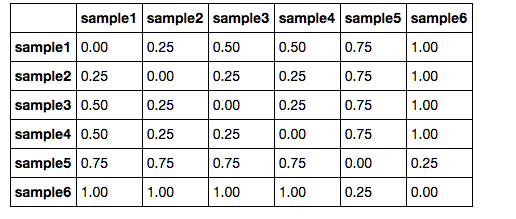
\includegraphics[width=4in]{./figures/simulated_real_matrix.png}}
\caption{\bf Dissimilarity matrix between synthetic samples using Bray-cutis from species composition directly }
\label{fig:simulated_real_matrix}
\end{figure}


\begin{figure}[!ht]
 \centerline{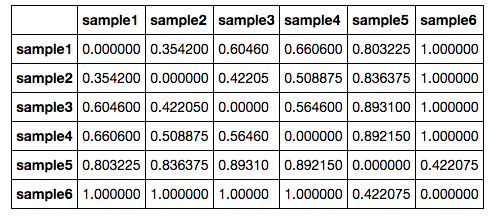
\includegraphics[width=4in]{./figures/simulated_matrix1.png}}
\caption{\bf Dissimilarity matrix between synthetic samples using Bray-cutis from sequencing reads using IGS method }
\label{fig:simulated_matrix1}
\end{figure}

\begin{figure}[!ht]
 \centerline{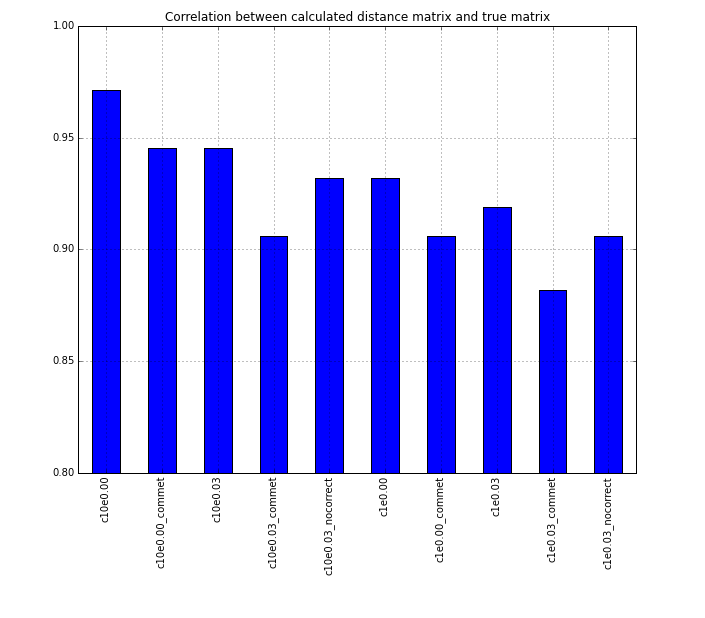
\includegraphics[width=4in]{./figures/IGS_correlation_methods.png}}
\caption{\bf Correlation between calculated distance matrix and true matrix from different data sets and using different methods}
\label{fig:IGS_correlation_methods}
\end{figure}


\begin{figure}[!ht]
 \centerline{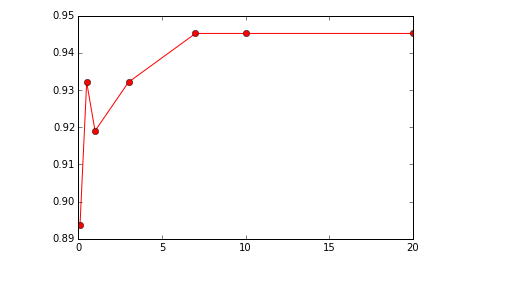
\includegraphics[width=4in]{./figures/IGS_correlation_coverage.png}}
\caption{\bf Correlation between calculated distance matrix and true matrix from different dat sets with different sequencing depth}
\label{fig:IGS_correlation_coverage}
\end{figure}


\subsubsection{Evaluate alpha diversity analysis by estimating size of metagenome}

We can use statistic metric to estimate the total number of IGSs in a sample, which can be used to calculate the estimated genome size of a sample using the formula below:
\\
size of genome = number of IGS x (reads\_length - k-size +1)\\
\\
Here we check how accurate the estimated size of genome and coverage is using different data sets with variable coverage/sequencing depth.

The genome size of the 6 samples should be:

sample1: AAAB 2x100K = 200K bp

sample2: AABC 3x100K = 300K bp

sample3: ABCD 4x100K = 400K bp

sample4: ABCE 4x100K = 400K bp

sample5: AFGH 4x100K = 400K bp

sample6: IFGH 4x100K = 400K bp

In this experiment, we use ACE metric since we find it is more accurate than Chao1, since it uses more abundance information.

Table \ref{fig:IGS_table_alpha1_10x_0} shows the estimated genome size of samples using error-free simulated sequencing data sets
is close to true size shown above. If the sequencing error is introduced, the estimated genome size is inflated dramatically as shown in Table \ref{fig:IGS_table_alpha1_10x_3_ne}, which is 
not surprising. However after applying error correction, we can still get good estimation of genome size, as shown in Table \ref{fig:IGS_table_alpha1_10x_3_e}.
This proves again error correction can improve the effectiveness of IGS method.

% test error rate 0.1?0.2?0.3? to see the influence of error rate???

Figure \ref{fig:IGS_table_alpha1_10x_3_e} shows the estimated genome size from data sets with variable coverage.
The estimated genome size keeps increasing as we use more reads, with higher coverage,which is  higher than actual genome size.
It's interesting that the estimated genome size is very high with low coverage, (probably due to more unique k-mers, which makes error correction more difficult. Then the estimated genome size drops a little bit as coverage from 0.1X to 1-3X, then starts to climb again as coverage increases, probably because there are always more erroneous k-mers that cannot be corrected. The good thing is that the climbing rate is not that high, this is believed to be due to the effectiveness of our error correction algorithms.

It is important to point that even though the absolute value of estimated genome size may be overestimated. The relative relationship between samples are reliable, as shown in the figure. Sample3,4,5,6 all have 4 species, while sample 2 has 3 species, and sample 1 has 2 species. They can be separately pretty well.


\begin{figure}[!ht]
 \centerline{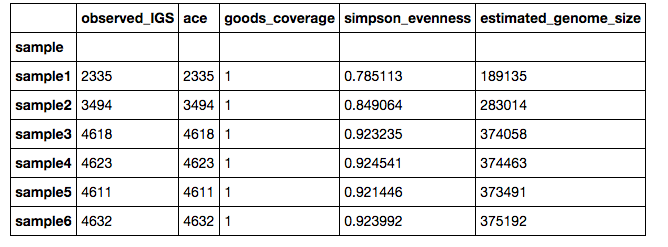
\includegraphics[width=4in]{./figures/IGS_table_alpha1_10x_0.png}}
\caption{\bf Coverage = 10x, No error}
\label{fig:IGS_table_alpha1_10x_0}
\end{figure}


\begin{figure}[!ht]
 \centerline{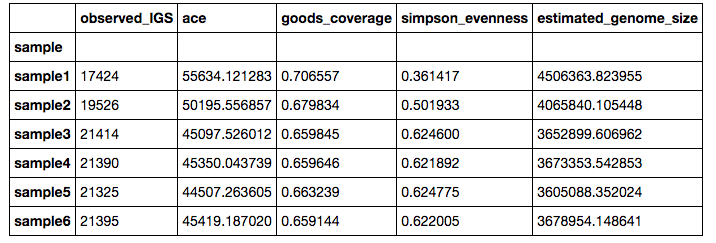
\includegraphics[width=4in]{./figures/IGS_table_alpha1_10x_3_ne.png}}
\caption{\bf Coverage = 10x, error = 3\%, no error correction}
\label{fig:IGS_table_alpha1_10x_3_ne}
\end{figure}



\begin{figure}[!ht]
 \centerline{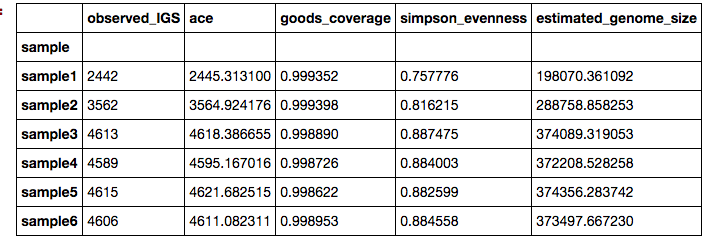
\includegraphics[width=4in]{./figures/IGS_table_alpha1_10x_3_e.png}}
\caption{\bf Coverage = 10x, error = 3\%, with error correction}
\label{fig:IGS_table_alpha1_10x_3_e}
\end{figure}

\begin{figure}[!ht]
 \centerline{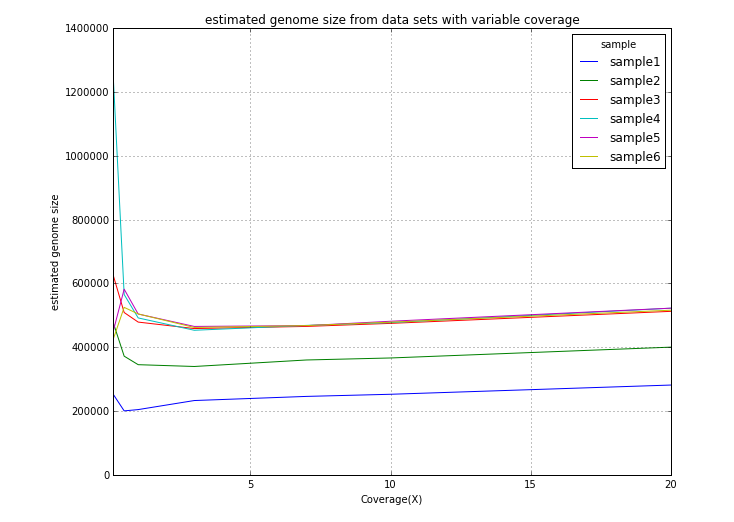
\includegraphics[width=4in]{./figures/IGS_figure_test_alpha.png}}
\caption{\bf estimated genome size from data sets with variable coverage}
\label{fig:IGS_figure_test_alpha}
\end{figure}


\subsection{The IGS method can provide a whole framework to do alpha or beta diversity, with good versatility.}

From the testing using simulated data sets shown here, we are confident that our IGS method works well and can give reliable results from data sets with error and low sequencing depth.

The IGS method can provide a whole framework to do alpha or beta diversity. Here we tested beta diversity using only bray-curtis metric and alpha diversity on richness only. Actually any metric can be applied to the IGS-by-samples table, abundance-based or incidence-baserd, richness or evenness.

Compareads(Commet) based on reads overlap between samples can get a matrix reflecting the real relationship between samples pretty good but it is stuck with one metric, which is based on the percentage of overlap reads between samples. This metric is like bray curtis , but not exactly the same.



\input{chap4-realdata}
%check the reads coverage in the sample where it is from
%
%\section{de bruijn graph mapping}
%
%check the reads coverage in another sample
%
%\section{IGS-based diversity analysis}
%


\chapter{Conclusion}

%Advantage:

%not only HMP, high depth, data
%but also low depth data, like soil metagenomics, which is impossible to use traditional method 


We have developed a novel statistical framework for enabling microbial diversty
 analysis using whole genome shotgun metagenomic reads data set without the
requirement of assembly, binning, reference or annotation. This dissertation
covers an overview of existing approaches of doing microbial diversity analysis
 of metagenomic samples, especially based on the concept of OTU, including the
steps in the procedure, like metagenomic assembly, contig binning, statistical
analysis of OTU abundance information to estimate the microbial diversity. Next
the statistical framwork based on the novel concept of IGS was discussed. As
the foundation of the framework, we described a novel method to count k-mers
efficiently and a scalable approache to retrieve the coverage of a read in a 
data set based on efficient and online k-mer counting. We also introduced the
application of this approach in reducing the redundancy of metagenomic reads
dataset, which is beneficialf to other tasks in metagenomic data analysis, like
assembly or error trimming. Finally, we discussed how we developed the concept 
of IGS based on the method of efficient k-mer counting and digital
normalization discussed before.  
The application of IGS to analyze microbial diversity of metagenomic data sets 
was discussed and the performance of the IGS method on simulated data sets and
real data sets were demonstrated in the final chapters. In this chapter, we
summarize how the novel statistical framwork based on IGS makes a difference to
 the diversity analysis in current microbial ecology research. 
Finally the possible avenues for future work will be discussed.

  

\section{Summary}

Diversity analysis is a key part of the microbial ecological research, like of
macroorganism ecology. However due to the obscure definition of the term
"species" in microbial ecology, we can virtually never measure the diversity of
species directly, rather we use other taxonomic concepts like operational
taxonomic unit (OTU) to evaluate the diversity of microbial community, instead
of species. rRNA sequencing reads may be classified into different OTUs.
Shotgun whole genome sequencing reads can also be classified into OTUs. But
most if not all
the existing methods based on the concept of OTU rely on some kinds of
preprocessing of original reads data like assembly or some kinds of external 
information like reference sequences for annotation. Both of the prerequisites
are not satisfied for many metagenomic project. For some low coverage
metagenomic reads data, assembly can only extract partial information from the
species with higher sequencing depth. It is common only a small proportion of
reads can be used in assembly. The reference sequence database is far from
completion enough especially for environmental sample from soil or sea water.
So applying these methods can only yield a partial picture of diversity of
the microbial community the metagenomic sequencing data covers. 

The IGS based
method discussed in this dissertation offers a brand new framework that
bypasses the difficult tasks like assembly, binning, or annotation whthout the
requirement of reference sequence database. It can take advanrage of all the 
information in the metagenomic reads data and gain a full picture of the
diversity of the microbial community. The fact that this is a whole new
framework with the concept of IGS to replace OTU as the taxinomic unit to
analyze diversity means that this framework can be used to do all the possible
diversity analysis that OTU-based framework can do. This is a more thorough
solution than many other methods that are developed to solve some specific
problems in the field of diversity analysis. For example, there are several
methods developed to estimate the richness of a metagenomic sample or the size 
of metagenome (cite nonparel,etc.) Our IGS based framework can not only
estimate the richness or size of metagenome as shown in the section above, but
also it can estimate the evenness or species abundance distribution of a
metagenomic sample, which is also an important aspect of alpha diversity
analysis. For beta diversity or compositional similarity analysis between
metagenomic samples, there are several methods developed to compare metagenomic
samples based on reads mapping or counting shared reads. (cite compareads)
But basically they only estimate abundance-based similarity, similar to
the Bray-Curtis indices used in the experiment discussed in the section above.
Actually what is not shown in the result in the section above is that the 
IGS-based framework can also be used to estimate incidence-based similarity, if
such information is interesting to the researcher.

Besides the advantage of the IGS based framework that it has a broad
application with its versatile potential, this freamework is also efficient and
highly scalable enough to handle extremely large metagenomic sequencing data
sets. We have discussed the efficiency of the novel k-mer counting method and
the following method of digital normalization, with the ability to retrieve the
coverage of a read accurately and efficiently. We also did thorough analysis
to the effect of the size of used data structure to the accuracy. We can take
advantage of the probabilitic characteristics of the data structure to make a
trade-off between expected analysis accuracy and expected usage of
computational power. In this way, we make the analysis highly scalable to
the increasing size of metagenomic sequencing data.  

Also, for the purpose of estimating microbial diversity of metagenomic samples,
we analyzed the effect of sequencing depth to the accuracy of the estimation.
It is obvious and expected that using more reads data with higher sequencing
depth increases the accuracy of such diversity estimation. Especially for beta
diversity or similarity analysis between samples, reads data with relatively
low sequencing depth can still yield decent result, as shown in the experiment
with synthetic data and real soil data set. For alpha diversity like richness
estimation, using reads data with lower sequencing depth gets the estimation
farther from the real number, but although the absolute value of such species
richness of a sample is not that accurate, the relative relationship of species
richness between samples are less prone to smaller reads data with lower
sequencing depth. These analysis and observation convince that for specific
purpose, only a subset of the large metagenomic reads data can be enough to
achieve reasonably satisfying result. Under certain circumstance, this feature
is quite helpful and can reduce the computational expense dramatically. 


\section{Future Work}


Though this dissertation detailed a new approach to analyze microbial diversity
using whole genome shotgun sequencing data without the requirement of assembly,
binning, or annotation, there is still plenty of room for improvement.  

Basically we question the IGS based method is developed to answer is how many
species there are in the sample or how similar the samples are between each
other, mostly focusing on the quantitative aspect. Admittedy these are 
important questions the microbial ecologists want to answer, they are also
curious to the qualitative questions, like if two samples are different, what
are the stuffs that attribute to the diffence,and what are the function of
those stuffs.cite rob knight's new paper.  A natural expansion of the IGS based framework will lead to
answer questions like this. 

Now we have an efficient and scalable approach to get the coverage of a read in
a sample, it is straightforward to extract the reads according to its coverage
profile across samples so we can get a subset of reads that have specific
characteristics, like the reads are common to all the samples. In this way we
may collect these "common" reads from samples together and try to co-assemble
them since now they should have higher coverage. Or we can get a subset of
reads that are common in a group of samples but do not exist in another group
of samples, like the samples from patients and healthy persons. These
"signiture" reads may offer important insights to understand what happens
to the microbial community while the environment changes. Admittedly these
kinds of "extraction" can be implimented using other methods like reads 
alignment method. But they may not be as efficient and scalable as the IGS
based method, especially for extremely large metagenomic data thanks to sliding
cost of sequencing.


One advantage of the IGS based method is that binning is not required in this
procedure. Firstly traditionally binning is used to classify contigs after some
kinds of assembly effort. The similarity based binning method relies on
sequence alignment, which is not efficient, especially infeasible for large
metagenomic data. Also, reference sequences normally are required for
similarity based binning approach. The composition-based approach relies on the
frequency profile of sequence signatures and machine learning approach on that
profile, which is computationally expensive. As reviewed in the second chapter,
the third approach based on coverage profile across samples was developed
recently. (cite concoct, groopm, etc.), although mostly often, the coverage
profile is used with the companion of composition frequency profile to classify
contigs. The assumption on which the coverage profile based binning approaches
are based on, that contigs with similar coverage profile across samples are
more likely to be from the same microbial organism, is actually similar to the
assumption on which using IGS to do beta diversity is based, that the IGSs with
similar coverage profile across samples are likely to be frome the same
microbial organism. It is promising to classify the IGSs by the coverage
profile across samples. We have already overcome the challenge of retrieving the
coverage profile efficiently based on the probabilistic data structure, while
in those coverage profile based binning approaches the coverage profile is 
normally retrieved by assembly of contigs and mapping
reads back to contigs, which both require higher coverage reads to do assembly
and are computationally expensive. 

There are two problems to deal with about this coverage profile based
IGS binning approach. First, with relatively small number of samples, the
resolution will be limited, since the total number of different coverage
profiles will be limited. This is probably the reason most of those coverage
profile based contig binning method integrate composition profile information
also. Second, on the other hand, if there are large number of samples, there
will be too many diferent coverage profiles. We can use more sophisticated
clustering approach to the coverage profiles to reduce the number of bins,
as in those coverage profile based contig binning methods. Another approach
worthy of note is that there is a method termed partitioning developed in
our lab as a divide and conque approach to scale metagenome assembly. It can be 
considered as a rough binning approach also, where the reads in the same
partition are more likely to originate from the same microbial organism. We can
try to integrate the paritioning and IGS coverage profile to improve the
accuracy of the binning. In summary, this will be one of the first attempts to
do reads binning. After the IGS/reads binning,  we expect to do better assembly
 and annotation expected to be more accurate to gain more knowledge about the
function and phylogenetical information.  

As shown in Figure, after adjustment according to sequencing error and collison
rate of the bloom filter, the estimated size of metagenome is close to real
number for synthetic data sets. But the difference between the estimation and
real number is still increasing with higher error rate, which means there is
other factor that affect the accuracy of estimaiton. This is worthy of further
investigation. This kind of estimation of metagenome is extremely important in
metagenomic data analysis and it is closely related to the estimation of
sequencing depth or how much more effort is required to gain enough sequencing
depth. As shown in the result, we are confident that the relative relationship 
between the richness of different samples are reliable from the IGS based alpha
diversity analysis. How accurate the absolute value of the richness or the size
of metagenome in a real data requires further research and new  
statistical model may be needed to adapt to the abundance distribution of IGSs.    
Furthermore, any information about the richness of a sample is beneficial to
the optimal choice of parameter for digital normalization.

The analysis of the effect of sequencing depth to the accuracy of beta
diversity shows that using a relatively small subset of the whole data set may
get reasonably good result showing the separation of samples after clustering
or ordination. However how good the seperation is seems to be related to the
characteristic of samples and can not be determined easily before starting the
analysis. So a potential approach is to do such beta analysis in an iterative
fasion. We already know that using more data will yield better result or better
separation for the purpose of comparing metagenomic samples. So in such
iteration procedure, how good the separation is can be monitored as more reads
are loaded into the analysis and the procedure can be stopped as long as the
pattern of the separation of samples is significant enough. This way, we may
save lots of computational expense and still have enough information about the
relationship between samples. 
 
    
    
    
    
    
    



%%%%%%%    APPENDICES    %%%%%%%%%%
%% If you wish to include one appendix, remove the "%" from the 
%% following two lines.
\renewcommand{\appname}{APPENDIX}
\appendix
\input{gloss}
%% To include several appendices, remove the only the "%"
%% in front of "\appendix".

%% In either cast to start your first appendix, which will be labeled
%% as Appendix A, just type \chapter{<appendix 1 name>}
%% and enter the text of the appendix as you would a chapter.

%%%%%%% A NOTE ABOUT APPENDICES %%%%%%%%%
%% Some appendices may be single spaced such as survey examples or letters.
%% Contact the Graduate School for details.
%% To single space an appendix first remove the % from 
%% the following two lines. 
% \end{doublespace}
% \chapter{<appendix  name>}
%% After entering the appendix remove the % from 
%% the following line
% \begin{doublespace}
%% Any text entered now will be double spaced.
\end{doublespace}

%%Bibliography 

%% A bibliography is required. By default it is called, "Bibliography"
%% You may use �Literature Cited�, �Works Cited� or �References� 
%% instead of �Bibliography� if that is the convention in your discipline. 
%% To do so, place your choice in the  empty argument 
%% of the following command and remove the "%".
\renewcommand{\bibname}{BIBLIOGRAPHY}
%% The bibliography may be made using BibTeX.
%% If it's made from scratch,
%% remove the "%" in front of "\begin{thebibliography}{???}"
%% replacing the ??? with the appropriate entry and 
%% remove the "%" in front of "\end{thebibliography}"
% \begin{thebibliography}{???}
%%  Enter the bibliography here.
% \end{thebibliography}

\bibliographystyle{abbrv}
\bibliography{dis}

\end{document}
